\chapter{径向量子化、共形算符与高自旋态}\label{chap:ghs-radial-highspin-states}
\label{chap:ghs-radial-quantization}
\label{chap:ghs-interaction-anomalous-dimensions}



在通常的场量子化中，我们先规定一个时间坐标，再问场在等时超曲面上有哪些自由度。研究共形场论时还有一种更合适的选择：如果在原点放置一个局域算符，然后向外逐渐扩大包围它的球面，那么球面内部所包含的信息就能够用球面上的量子态表示。向外移动球面的动作，在共形理论里恰好由尺度变换生成。这样，局域算符的标度维数便可能直接成为某个哈密顿量的能量本征值。

前章已从反射正性与谱演算建立自由量子态。现在要求平直空间的共形对称和局域真空扇区，使扩张球面的边界演化成为尺度变换。双粒子高自旋态将在这一条件下从初级条件构造，随后再由局域相关函数研究相互作用如何改变其表示。

下面采用 $d>2$ 维欧氏平直空间，指标 $\mu,\nu=1,\ldots,d$，度规 $\delta_{\mu\nu}$。空间点写成 $x^\mu=r n^\mu$，其中 $r=|x|>0$，$\vb n\in S^{d-1}$ 且 $n^\mu n_\mu=1$。球面角测度 $\dd\Omega_{d-1}$ 的总面积记为 $\Omega_{d-1}=2\pi^{d/2}/\Gamma(d/2)$。固定一个任意的参考长度 $R>0$，定义无量纲径向时间
\begin{equation}\label{eq:ghs-radial-time}
 u=\log\frac rR,\qquad r=R\ee^u.
\end{equation}
$u\to-\infty$ 是原点，而不是普通直角坐标 $x^d$ 方向的远处。尤其不能把它与真实实验室时间混为一谈。


平直度规在球坐标下为 $\dd s^2=\dd r^2+r^2\dd\Omega_{d-1}^2$。由 $\dd r=r\dd u$ 得
\begin{equation}\label{eq:ghs-weyl-cylinder}
 \dd s^2=r^2\bigl(\dd u^2+\dd\Omega_{d-1}^2\bigr),\qquad
 \dd^d x=r^d\dd u\,\dd\Omega_{d-1}.
\end{equation}
圆柱上的每一条时间截面都是同一个单位球面。这不是等距变换，因为右侧还有随 $u$ 改变的尺度因子 $r^2$；只有在共形理论允许局域度规重标度时，才能把两种描述联系起来。以半径 $R$ 为几何单位，圆柱的物理度规可取 $\dd s_{\rm cyl}^2=R^2(\dd u^2+\dd\Omega_{d-1}^2)$。

\begin{figure}[htbp]
\centering
% Local TikZ geometry; styles inherited exclusively from the shared preamble.
\begin{tikzfig}[scale=.95]
\draw[thick] (-2.5,0) circle (1.47);
\draw[thick] (-2.5,0) circle (.94);
\draw[thick] (-2.5,0) circle (.39);
\draw[lecturearrow] (-2.5,0)--(-1.07,0) node[midway,above] {$r$};
\node[lecturelabel] at (-2.5,-2.05) {$\mathbb R^d\setminus\{0\}$};
\draw[lecturearrow] (-.5,0)--(.72,0) node[midway,above] {Weyl};
\draw[thick] (1.45,-1.52) rectangle (4.05,1.52);
\draw[thick] (1.45,-.73)--(4.05,-.73) (1.45,.29)--(4.05,.29);
\draw[gray,dashed] (1.45,-.32)--(4.05,-.32);
\draw[lecturearrow] (4.43,-1.25)--(4.43,1.25) node[above] {$u$};
\node[lecturelabel] at (2.75,1.9) {$\mathbb R\times S^{d-1}$};
\node[lecturelabel] at (2.75,-2) {$u=\log(r/R)$};
\end{tikzfig}

\caption{除原点平直空间的同心球面与圆柱等时截面的对应。$u=\log(r/R)$ 使径向缩放变成柱面平移；二者通过 Weyl 因子而非等距变换联系。}\label{fig:ghs-radial-annulus-cylinder}
\end{figure}

\cref{fig:ghs-radial-annulus-cylinder} 强调了 $r\to0$ 被拉到 $u\to-\infty$。这也是为什么原点的局域算符在圆柱语言下表现为从远过去准备出的态。

对于标度维数为 $\Delta_{\mathcal O}$ 的标量初级算符，其圆柱对应量定义为 $\mathcal O_{\rm cyl}(u,\vb n)=r^{\Delta_{\mathcal O}}\mathcal O(r\vb n)$。这里的长度幂将场变成无量纲对象，便利于以下的光谱计算。带自旋的初级算符还需要按所选局部正交标架变换指标；不能对任意张量都只乘一个尺度因子。


设 $\varphi$ 是归一化后的无质量自由实标量场，其欧氏无量纲作用量为
\begin{equation}\label{eq:ghs-flat-action}
 \mathscr I[\varphi]=\frac12\int_{\RR^d}\dd^d x\,\delta^{\mu\nu}
 \partial_\mu\varphi\,\partial_\nu\varphi,
 \qquad \Delta_\varphi\equiv\delta=\frac{d-2}{2}.
\end{equation}
$\mathscr I=I_E/\hbar$，因此泛函积分权重是 $\exp(-\mathscr I)$；$[\varphi]=\mathrm{length}^{-\delta}$。我们将无量纲圆柱场定义为 $\Phi(u,\vb n)=r^\delta\varphi(r\vb n)$。可直接计算
\begin{align*}
 \partial_r\varphi&=r^{-\delta-1}(\partial_u\Phi-\delta\Phi),\\
 \nabla_{S^{d-1}}\varphi&=r^{-\delta}\nabla_{S^{d-1}}\Phi,\\
 |\nabla_{\RR^d}\varphi|^2&=r^{-2\delta-2}
 \left[(\partial_u\Phi-\delta\Phi)^2+|\nabla_{S^{d-1}}\Phi|^2\right].
\end{align*}
测度给出 $r^d$，而 $d-2\delta-2=0$，所以全部显式径向因子消失。含全导数的完整结果是
\begin{align}\label{eq:ghs-cylinder-action}
 \mathscr I&=\frac12\int\dd u\,\dd\Omega_{d-1}
 \left[(\partial_u\Phi)^2+|\nabla_{S^{d-1}}\Phi|^2+\delta^2\Phi^2\right]
 -\frac\delta2\int\dd\Omega_{d-1}\,[\Phi^2]_{u_-}^{u_+}.
\end{align}
最后一项来自 $-2\delta\Phi\partial_u\Phi=-\delta\partial_u(\Phi^2)$。它在有限时间区间并不恒为零；在固定边界数据的传播核中，它改变的是边界波泛函的归一化，而非圆柱体内的运动方程。

为什么没有质量的平直场，会在圆柱作用量中出现 $\delta^2\Phi^2$？圆柱标量曲率为 $\mathcal R_{\rm cyl}=(d-1)(d-2)/R^2$，共形耦合系数为
\begin{equation}\label{eq:ghs-conformal-coupling}
 \xi_d=\frac{d-2}{4(d-1)},\qquad
 R^2\xi_d\mathcal R_{\rm cyl}=\delta^2.
\end{equation}
故这是一项几何曲率耦合，不是平直时空中凭空增加的粒子质量。若漏掉它，整个径向谱便会算错。


在平直极限，上式可以直接化为熟悉的自由场方程。
对一般背景度规 $g_{\mu\nu}$，与自由共形标量对应的二次型包含
\begin{proof}
\begin{equation*}
\frac12\int\dd^d x\sqrt g\,\bigl[g^{\mu\nu}\partial_\mu\varphi\partial_\nu\varphi+\xi_d\mathcal R\varphi^2\bigr].
\end{equation*}
在平直空间 $\mathcal R=0$。Weyl 变换 $g_{\mu\nu}=\ee^{2\sigma}\widehat g_{\mu\nu}$ 下，若 $\varphi=\ee^{-\delta\sigma}\widehat\varphi$，曲率 $\mathcal R$ 的变换和标量梯度展开互相抵消所有体内的 $\nabla\sigma$ 项，至多相差边界项。这里 $\sigma=u+\log R$，所得体内二次型与 \cref{eq:ghs-cylinder-action} 一致。直接代入法也表明该等价不要求预先假定曲率变换公式。
\end{proof}

对欧氏圆柱作解析延拓 $u=\ii t/R$（此处 $t$ 是具有长度量纲的洛伦兹时间坐标；物理时间为 $t/c$）。相应的频率将以 $1/R$ 为单位。为了简化推导，后续先使用无量纲圆柱洛伦兹时间 $\tau=ct_{\rm phys}/R$；所有能量本征值先以无量纲数 $E$ 表示，相对于圆柱真空的物理激发能量则是
\begin{equation}\label{eq:ghs-physical-energy}
 E_{\rm phys}=\frac{\hbar c}{R}E,
 \qquad \Omega_{\rm phys}=\frac cR\,\omega.
\end{equation}
这使理论中 $\hbar,c$ 的位置明确，也避免把标度维数误当成具有焦耳量纲的能量。

四维实际标量场 $\phi_{\rm phys}$ 若选取闵可夫斯基作用量 $S=\frac12\int\dd t_{\rm phys}\dd^3\vb x[(\partial_t\phi_{\rm phys})^2/c^2-|\nabla\phi_{\rm phys}|^2]$，则其欧氏作用量满足 $I_E/\hbar=\frac12\int\dd^4x_E|\nabla(\phi_{\rm phys}/\sqrt{\hbar c})|^2$，其中 $x_E^0=ct_E$。因而四维的 $\varphi=\phi_{\rm phys}/\sqrt{\hbar c}$，且 $\Phi=r\phi_{\rm phys}/\sqrt{\hbar c}$。后文出现的 $C_d$ 是这一归一化场的二点函数系数。


\section{圆柱谱与局域算符}
\label{sec:ghs-cylinder-spectrum}


从这里起以参考半径 $R$ 为长度单位，令 $x/R$ 记作 $x$、$R^\delta\varphi$ 仍记作 $\varphi$，导数相应无量纲化；物理单位由 \cref{eq:ghs-physical-energy} 恢复。一个圆柱时间切片上的场不是有限维粒子坐标，而是定义在 $S^{d-1}$ 上的函数。把它按球谐函数分解，便可以逐个辨认自由度。更重要的是，这个分解可以在不预设态—算符对应的情况下，直接算出原点插入产生了哪个态。


令 $Y_{\ell a}(\vb n)$ 为实的正交归一球谐函数，$\ell\in\NN_0$，$a=1,\ldots,g_{d,\ell}$。约定
\begin{equation}\label{eq:ghs-sphere-spectrum}
 -\Delta_{S^{d-1}}Y_{\ell a}=\ell(\ell+d-2)Y_{\ell a},\qquad
 \int_{S^{d-1}}\dd\Omega\,Y_{\ell a}Y_{\ell'a'}=\delta_{\ell\ell'}\delta_{aa'}.
\end{equation}
这个谱由平直空间的拉普拉斯算符直接得到：
\begin{align*}
 \Delta_{\RR^d}&=\partial_r^2+\frac{d-1}{r}\partial_r+\frac1{r^2}\Delta_{S^{d-1}},\\
 0=\Delta_{\RR^d}(r^\ell Y_{\ell a})
 &=r^{\ell-2}[\ell(\ell+d-2)+\Delta_{S^{d-1}}]Y_{\ell a}.
\end{align*}
这里 $r^\ell Y_{\ell a}$ 正是 $d$ 维调和齐次多项式。其简并度等于所有 $\ell$ 次齐次多项式数目减去可被 $r^2$ 整除的部分：
\begin{equation}\label{eq:ghs-sphere-degeneracy}
 g_{d,\ell}=\binom{\ell+d-1}{\ell}-\binom{\ell+d-3}{\ell-2}
 =\frac{(2\ell+d-2)(\ell+d-3)!}{\ell!(d-2)!},
\end{equation}
第二个二项式在 $\ell<2$ 时取零。特别地，四维球面 $S^3$ 上 $g_{4,\ell}=(\ell+1)^2$。

\begin{figure}[htbp]
\centering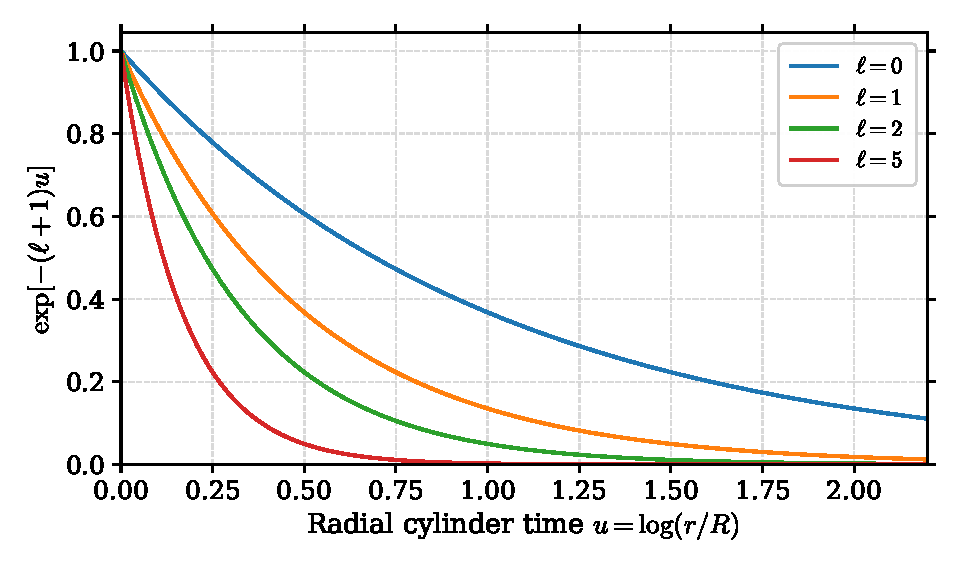
\includegraphics[width=.79\linewidth]{content/FreeElectronQuantumOptics/figures/geometry-highspin/generated/cylinder_mode_decay.pdf}
\caption{四维共形自由标量圆柱上的模态因子 $\exp[-(\ell+1)u]$（$u\ge0$）。高角动量模态随径向时间衰减得更快，但这种指数谱依赖标准球面的共形频率，不能照搬到任意截面。}\label{fig:ghs-cylinder-mode-decay}
\end{figure}

\cref{fig:ghs-cylinder-mode-decay} 将圆柱 哈密顿量 的离散频率和径向传播因子直观联系起来；在一般截面上必须以具体算子 $A_h$ 的谱替换 $\ell+1$。


由 \cref{eq:ghs-cylinder-action} 去掉边界项并解析延拓，圆柱洛伦兹拉格朗日量是
\begin{equation*}
 L=\frac12\int\dd\Omega\,
 \left[(\partial_\tau\Phi)^2-|\nabla_{S^{d-1}}\Phi|^2-\delta^2\Phi^2\right].
\end{equation*}
写成 $\Phi(\tau,\vb n)=\sum_{\ell,a}q_{\ell a}(\tau)Y_{\ell a}(\vb n)$，各模正交性使拉格朗日量对角化：
\begin{align}\label{eq:ghs-harmonic-oscillators}
 L&=\frac12\sum_{\ell,a}[\dot q_{\ell a}^2-\omega_\ell^2q_{\ell a}^2],\\
 \omega_\ell^2&=\ell(\ell+d-2)+\delta^2=(\ell+\delta)^2.\notag
\end{align}
$\omega_\ell>0$，因为 $d>2$。取 $[q_{\ell a},p_{\ell'a'}]=\ii\delta_{\ell\ell'}\delta_{aa'}$ 与 $p_{\ell a}=\dot q_{\ell a}$，引入满足 $[a_{\ell a},a_{\ell'a'}^\dagger]=\delta_{\ell\ell'}\delta_{aa'}$ 的振子，得到
\begin{align}\label{eq:ghs-field-expansion}
 \Phi(\tau,\vb n)&=\sum_{\ell,a}\frac{Y_{\ell a}(\vb n)}{\sqrt{2\omega_\ell}}
 \left[a_{\ell a}\ee^{-\ii\omega_\ell\tau}+a_{\ell a}^\dagger\ee^{\ii\omega_\ell\tau}\right],\\
 \widehat D&=\sum_{\ell,a}(\ell+\delta)a_{\ell a}^\dagger a_{\ell a}.
 \label{eq:ghs-dimension-operator}
\end{align}
圆柱真空 $|0\rangle$ 满足 $a_{\ell a}|0\rangle=0$。$\widehat D$ 是按真空能量取零的尺度生成元；在偶数维的曲背景上，绝对真空能量还可能含有依赖重整化约定的 Casimir 项，这不改变上述激发能量差。它也等于圆柱哈密顿量乘以 $R/(\hbar c)$，故每增加一个球谐激发，能量就增加 $(\ell+\delta)\hbar c/R$。


自由场满足 $-\Delta_{\RR^d}G(x)=\delta^{(d)}(x)$，衰减的欧氏 Green 函数为
\begin{equation}\label{eq:ghs-propagator}
 G(x-y)=\langle\varphi(x)\varphi(y)\rangle
 =\frac{C_d}{|x-y|^{2\delta}},\qquad
 C_d=\frac{\Gamma(\delta)}{4\pi^{d/2}}.
\end{equation}
由于在 $r>r'$ 的球面上可以依 $\ell$ 分解传播子，同一个函数也必须有模式展开
\begin{equation}\label{eq:ghs-propagator-modes}
 G(r\vb n,r'\vb n')=\sum_{\ell,a}\frac{Y_{\ell a}(\vb n)Y_{\ell a}(\vb n')}{2(\ell+\delta)}
 \frac{(r')^\ell}{r^{\ell+2\delta}},\qquad r>r'.
\end{equation}
这一步不仅验证频率，也检验了 \cref{eq:ghs-field-expansion} 中的 $1/\sqrt{2\omega_\ell}$。


利用 Gegenbauer 多项式的生成函数，可逐项读出传播子的模态。
记 $t=r'/r<1$，$v=\vb n\cdot\vb n'$。Gegenbauer 多项式的生成函数给出
\begin{proof}
\begin{equation*}
(1-2tv+t^2)^{-\delta}=\sum_{\ell=0}^\infty C_\ell^{(\delta)}(v)t^\ell.
\end{equation*}
球谐加法定理在我们的正交归一约定下为
\begin{equation*}
\sum_aY_{\ell a}(\vb n)Y_{\ell a}(\vb n')
=\frac{\ell+\delta}{\delta\Omega_{d-1}}C_\ell^{(\delta)}(v).
\end{equation*}
由 $\delta\Omega_{d-1}C_d=1/2$，右侧除以 $2(\ell+\delta)$ 后恰好变成 $C_d C_\ell^{(\delta)}(v)$，从而逐项恢复 \cref{eq:ghs-propagator}。加法定理的系数在 $v=1$ 可由 $\sum_aY_{\ell a}(\vb n)^2=g_{d,\ell}/\Omega_{d-1}$ 和 $C_\ell^{(\delta)}(1)=(2\delta)_\ell/\ell!$ 独立核对。
\end{proof}

欧氏时间演化把 \cref{eq:ghs-field-expansion} 写为
\begin{equation}\label{eq:ghs-radial-field-expansion}
 \varphi(r\vb n)=\sum_{\ell,a}\frac{Y_{\ell a}(\vb n)}{\sqrt{2(\ell+\delta)}}
 \bigl(a_{\ell a}r^{-\ell-2\delta}+a_{\ell a}^\dagger r^\ell\bigr),
\end{equation}
这里的 $r$ 已表示以 $R$ 为单位的无量纲径向坐标；对于物理场，右端还须恢复整体因子 $R^{-\delta}$。作用在真空上只剩产生部分。于是 $\partial_{\mu_1}\cdots\partial_{\mu_k}\varphi(0)|0\rangle$ 只从 $\ell=k$ 项得到贡献，因为 $r^\ell Y_{\ell a}(\vb n)$ 是 $\ell$ 次齐次多项式，对原点求 $k$ 阶导数时只有 $\ell=k$ 的项不为零。

选定两个正交单位向量 $\vb e_1,\vb e_2$，令复零极化向量 $\vb\varepsilon=\vb e_1+\ii\vb e_2$，于是 $\vb\varepsilon\cdot\vb\varepsilon=0$。记 $D_+=\vb\varepsilon\cdot\nabla$，则
\begin{equation}\label{eq:ghs-oneparticle-dimension}
 \widehat D\,D_+^k\varphi(0)|0\rangle
 =(k+\delta)D_+^k\varphi(0)|0\rangle.
\end{equation}
因为 $D_+^k$ 自动去除所有迹，该态位于 $\ell=k$ 的对称无迹张量表示中。$\varphi(0)|0\rangle$ 是 $\ell=0$ 最低态；加入空间导数会提高球谐阶数和圆柱能量。


径向量子化通过单位球内的欧氏路径积分制备一个球面态。局域插入 $\mathcal O(0)$ 的定义是 $|\mathcal O\rangle=\mathcal O(0)|0\rangle$，但态的内积不能用同一点处的算符乘积直接给出：其共轭插入必须先经球反演移动到无穷远。标量初级算符采用
\begin{equation}\label{eq:ghs-radial-adjoint}
 \langle\mathcal O|=\lim_{r\to\infty}r^{2\Delta_{\mathcal O}}
 \langle0|\mathcal O^\dagger(r\vb n),\qquad
 \|\mathcal O\|^2=\lim_{r\to\infty}r^{2\Delta_{\mathcal O}}
 \langle\mathcal O^\dagger(r\vb n)\mathcal O(0)\rangle.
\end{equation}
对于旋转张量，反演还作用于各指标，因此不应机械套用这个标量公式；以下将改用已经正交归一的球面振子求高自旋态范数。完整态—算符对应还以反射正性和选定的局域真空扇区为前提，参见文末文献 \cite{ghs-rychkov,ghs-simmons}。

\subsection{径向伴随与后裔的局部代数}

从正的径向内积选出初级态，需要知道平移和特殊共形生成元怎样互为伴随。共形表示的完整分类可参照《群论》的共形对称与最高权表示章；这里建立后续范数计算所需的关系。

\begin{definition}[径向共形生成元]
取实旋转生成元 $M_{\mu\nu}=-M_{\nu\mu}$、尺度生成元 $D$、平移 $P_\mu$ 和特殊共形生成元 $K_\mu$。它们满足
\begin{align}\label{eq:ghs-conformal-commutators}
 [D,P_\mu]&=P_\mu,&[D,K_\mu]&=-K_\mu,\\
 [K_\mu,P_\nu]&=2\delta_{\mu\nu}D-2M_{\mu\nu},&
 [M_{\mu\nu},P_\rho]&=\delta_{\nu\rho}P_\mu-\delta_{\mu\rho}P_\nu.\notag
\end{align}
在反射正的径向态空间中，球面反演把平移映为特殊共形变换，因此
\begin{equation}\label{eq:ghs-radial-generator-adjoint}
 D^\dagger=D,\qquad P_\mu^\dagger=K_\mu,\qquad M_{\mu\nu}^\dagger=-M_{\mu\nu}.
\end{equation}
$D$ 的本征值无量纲，圆柱物理能量差为 $\hbar c\Delta/R$。$M$ 与带虚数因子的厄密角动量算符采用不同约定。
\end{definition}

\begin{proposition}[幺正界与散度范数]
归一化标量初级态 $|\mathcal O\rangle$ 满足 $K_\mu|\mathcal O\rangle=0$、$D|\mathcal O\rangle=\Delta|\mathcal O\rangle$，则
\begin{equation}\label{eq:ghs-scalar-level-one-gram}
 \langle P_\mu\mathcal O|P_\nu\mathcal O\rangle=2\Delta\delta_{\mu\nu},\qquad
 \|P^2|\mathcal O\rangle\|^2=8d\Delta\left(\Delta-\frac{d-2}{2}\right).
\end{equation}
非恒等标量满足
\begin{equation}\label{eq:ghs-scalar-unitarity-bound}
 \Delta\ge\frac{d-2}{2}.
\end{equation}
对秩 $S\ge1$ 的非零对称无迹初级态，散度后裔满足
\begin{equation}\label{eq:ghs-spin-unitarity-bound-extended}
 \sum\|P^\nu|J_{\nu\mu_2\cdots\mu_S}\rangle\|^2
 =2(\Delta-S-d+2)\sum\|J_{\mu_1\cdots\mu_S}\rangle\|^2,
 \qquad\Delta\ge S+d-2.
\end{equation}
求和按有序张量指标进行；饱和时散度后裔在零范数商空间中消失。
\end{proposition}
\begin{proof}
由 $P^\dagger=K$，一级 Gram 矩阵为 $\langle\mathcal O|[K_\mu,P_\nu]|\mathcal O\rangle$，标量旋转项为零。对迹后裔，逐次交换给出
\begin{align*}
 K_\mu P^2|\mathcal O\rangle
 &=2DP_\mu|\mathcal O\rangle-2M_{\mu\nu}P_\nu|\mathcal O\rangle
   +2P_\mu D|\mathcal O\rangle\\
 &=\bigl[2(\Delta+1)-2(d-1)+2\Delta\bigr]P_\mu|\mathcal O\rangle.
\end{align*}
再左乘 $\langle\mathcal O|K_\mu$ 求和，恢复所述二级范数。

记 $L_{\mu_2\cdots\mu_S}=P^\nu J_{\nu\mu_2\cdots\mu_S}$。旋转生成元在首指标的收缩给出 $(d-1)J_{\alpha\mu_2\cdots}$；其余 $S-1$ 个指标各贡献一个相同张量，含两次重复指标的项由无迹性消去。因此
\[
 K_\alpha|L_{\mu_2\cdots}\rangle=2(\Delta-S-d+2)|J_{\alpha\mu_2\cdots}\rangle.
\]
左乘 $\langle J_{\alpha\mu_2\cdots}|$ 求和得到散度范数恒等式，正性给出下界。
\end{proof}


局域算符在球面上制备一个径向态，圆柱尺度生成元给出它的能量。但是固定能量和旋转权重以后，带导数的双粒子态仍然不唯一；选出共形初级态需要进一步施加特殊共形生成元的条件。

\section{共形初级态}
\label{sec:ghs-conformal-primary-bilinear}


球面振子告诉我们，给两个自由粒子一共分配 $S$ 个导数，得到的所有双粒子态都具有相同的圆柱能量 $2\delta+S$。但这还没有指定唯一的算符：$S$ 个导数可以以不同的方式分给两个场。单靠旋转权重和能量本征值，并不能选出一个真正的共形初级态。缺少的条件来自特殊共形变换。


在复零极化 $\vb\varepsilon=\vb e_1+\ii\vb e_2$ 下，任意秩 $S$ 对称无迹张量 $J_{\mu_1\cdots\mu_S}(x)$ 可收缩成多项式 $J_S(x;\vb\varepsilon)=\varepsilon^{\mu_1}\cdots\varepsilon^{\mu_S}J_{\mu_1\cdots\mu_S}(x)$。由于 $\varepsilon^2=0$，所有含度规的迹项都自动消失。多项式在整个零锥上给出的信息，可唯一确定原来的对称无迹张量。

在写二粒子态的系数以前，还应区分未对称的张量积和真正的玻色 Fock 态。设 $\mathcal H_1$ 是单粒子 Hilbert 空间，$u,v\in\mathcal H_1$，则
\[
 a^\dagger(u)a^\dagger(v)|0\rangle
 \longleftrightarrow \frac{u\otimes v+v\otimes u}{\sqrt2}
\]
右侧采用标准张量积内积与相应的玻色对称化映射。由正则对易关系，
\[
 \|a^\dagger(u)a^\dagger(v)|0\rangle\|^2
 =\|u\|^2\|v\|^2+|\langle u,v\rangle|^2.
\]
这说明两个模式均归一化且正交时，范数平方为一；两个归一化模式重合时，范数平方为二。后文对 $k$ 与 $S-k$ 的求和必须保留交换项；否则即使共形初级条件的递推完全正确，双粒子态的最终范数和单体概率也会错一个系数。该关系对任何截面的单粒子 Hilbert 空间成立，不依赖角动量基底。

定义旋转生成元的约定为




\begin{equation*}
 [J_{12},\varphi(x)]=\ii(x^1\partial_2-x^2\partial_1)\varphi(x).
\end{equation*}
在原点作用一次导数便得到 $[J_{12},D_+\varphi(0)]=D_+\varphi(0)$；归纳后，$D_+^k\varphi$ 的权重是 $k$。因此
\begin{equation}\label{eq:ghs-bilinear-general}
 \mathcal O_S(x;\vb\varepsilon)=\sum_{k=0}^{S}c_k:
 (D_+^k\varphi)(D_+^{S-k}\varphi):(x)
\end{equation}
的每一项都具有最高旋转权重 $S$，且标度维数为
\begin{equation}\label{eq:ghs-spin-energy}
 \Delta_S=2\delta+S=d-2+S,\qquad
 \widehat D|\mathcal O_S\rangle=\Delta_S|\mathcal O_S\rangle.
\end{equation}
这里冒号表示按真空正规序，不允许同一算符内两场自收缩。对自由理论，它确实创造恰好两个振子量子。


\begin{proposition}[初级条件与导数分配系数]
标量共形初级场在欧氏空间的特殊共形变换取约定
\begin{equation}\label{eq:ghs-K-scalar}
 [K_\mu,\varphi(x)]=
 [2x_\mu(x\cdot\partial+\delta)-x^2\partial_\mu]\varphi(x).
\end{equation}
真正的初级算符须在原点满足 $[K_\mu,\mathcal O_S(0)]=0$。设 $K_-=K_1-\ii K_2$，$x_-=x^1-\ii x^2$。由于 $D_+x_-=2$，$D_+(x^2)=2(x^1+\ii x^2)$，而 $D_+^2(x^2)=2\varepsilon^2=0$，可直接对 \cref{eq:ghs-K-scalar} 连续求导。得到最关键的对易式
\begin{equation}\label{eq:ghs-K-derivative}
 [K_-,D_+^k\varphi(0)]=4k(\delta+k-1)D_+^{k-1}\varphi(0),\qquad k\ge1.
\end{equation}
在最高权子空间里其余 $K_\mu$ 的作用为零（对 $K_1,K_2$，可用 $K_\pm$ 的两个组合核对；垂直分量由自由标量的导数结构消失）。

将 \cref{eq:ghs-K-derivative} 代入 \cref{eq:ghs-bilinear-general}，再把乘积写成含 $j$ 与 $S-1-j$ 阶导数的项。每个独立的双场单项式的系数必须为零，因此
\begin{equation}\label{eq:ghs-primary-recurrence}
 (j+1)(\delta+j)c_{j+1}
 +(S-j)(\delta+S-j-1)c_j=0,
 \quad j=0,\ldots,S-1.
\end{equation}
这是一阶递推关系，除总体倍数以外完全固定高自旋初级态。选 $c_0=1$，令 $(a)_k=\Gamma(a+k)/\Gamma(a)$，求得
\begin{equation}\label{eq:ghs-primary-coefficients}
 c_k=(-1)^k\binom Sk\frac{(\delta+S-k)_k}{(\delta)_k}
 =(-1)^k\binom Sk\frac{(\delta)_S}{(\delta)_k(\delta)_{S-k}}.
\end{equation}
特别地 $d=4$ 时 $\delta=1$，得到
\begin{equation}\label{eq:ghs-four-d-current}
 \mathcal O_S=\sum_{k=0}^S(-1)^k\binom Sk^2
 :(D_+^k\varphi)(D_+^{S-k}\varphi):.
\end{equation}
\end{proposition}

\begin{proof}
首先把 \cref{eq:ghs-K-scalar} 分为 $2\delta x_-\varphi$、$2x_-(x\cdot\partial)\varphi$ 和 $-x^2\partial_-\varphi$。原点处的 $k$ 次 $D_+$ 导数分别是
\begin{align*}
2\delta D_+^k(x_-\varphi)|_0&=4\delta k D_+^{k-1}\varphi(0),\\
2D_+^k[x_-(x\cdot\partial)\varphi]|_0
&=4k(k-1)D_+^{k-1}\varphi(0),\\
D_+^k[x^2\partial_-\varphi]|_0&=0.
\end{align*}
第二行里，$D_+(x\cdot\partial)\varphi|_0=D_+\varphi(0)$，所以多出的因子是 $k-1$。第三行为零是因为 $D_+^2x^2=0$ 且 $D_+x^2|_0=0$。合并前三式给出 \cref{eq:ghs-K-derivative}。

对一个乘积 $A_kB_{S-k}$，$K_-$ 可降低左边导数阶数，也可降低右边阶数。固定最终阶数为 $(j,S-1-j)$，左边由 $k=j+1$ 贡献 $4(j+1)(\delta+j)c_{j+1}$，右边由 $k=j$ 贡献 $4(S-j)(\delta+S-j-1)c_j$。两项相消便是 \cref{eq:ghs-primary-recurrence}。递推 $k$ 次后
\begin{align*}
c_k&=(-1)^k\prod_{j=0}^{k-1}\frac{(S-j)(\delta+S-j-1)}{(j+1)(\delta+j)}\\
&=(-1)^k\frac{S!}{k!(S-k)!}\frac{\Gamma(\delta+S)}{\Gamma(\delta+S-k)}
\frac{\Gamma(\delta)}{\Gamma(\delta+k)}.
\end{align*}
这也明确了 $d>2$ 时分母不会消失。
\end{proof}

\cref{eq:ghs-primary-coefficients} 中的两个阶乘分母关于 $k\leftrightarrow S-k$ 对称，故 $c_{S-k}=(-1)^S c_k$。由于两场相同，正规序后的两个因子可以交换，原算符又必须满足 $\mathcal O_S=(-1)^S\mathcal O_S$。对于奇数 $S$，它因而恒等于零。对于偶数 $S$，这是一个非平凡的初级态。

例如
\begin{align}\label{eq:ghs-spin-two-current}
 \mathcal O_0&=:\!\varphi^2\!:,\\
 \mathcal O_2&=2:\!\varphi D_+^2\varphi\!:
 -\frac{2(\delta+1)}{\delta}:\!(D_+\varphi)^2\!: .\notag
\end{align}
四维时第二式为 $2:\!\varphi D_+^2\varphi\!:-4:\!(D_+\varphi)^2\!:$。如果两种标量场不同，交换两因子不再是算符恒等变换，因此奇自旋混合双线性可以存在。


把 $D_+$ 作用在第一个场的动作形式地记为 $p$，作用在第二个场的动作记为 $q$。系数的生成多项式是 $F_S(p,q)=\sum_{k=0}^S c_kp^kq^{S-k}$。Jacobi 多项式的标准二项式展开恰好给出
\begin{equation}\label{eq:ghs-jacobi-polynomial}
 F_S(p,q)=\frac{S!\Gamma(\delta)}{\Gamma(S+\delta)}
 (p+q)^S P_S^{(\delta-1,\delta-1)}
 \!\left(\frac{q-p}{p+q}\right).
\end{equation}
右侧虽然出现 $p+q$ 的分母，但乘开以后它是严格的齐次多项式；在 $p+q=0$ 处按多项式延拓定义。由 Jacobi 与 Gegenbauer 多项式的关系，它亦可改写为 Gegenbauer 形式；当 $\delta=1$ 时，$P_S^{(0,0)}$ 就是 Legendre 多项式。

这个多项式不是凭空引入的特殊函数。它的系数之所以出现，完全由 \cref{eq:ghs-primary-recurrence} 的共形初级条件决定。由此也能理解高自旋流与特殊函数理论的关系：不同粒子之间分配导数的权重，正是一组正交多项式的展开系数。


对于一个幺正的 $d>2$ 维共形场论，非零自旋 $S\ge1$ 的对称无迹初级算符满足表示论下界 $\Delta_S\ge S+d-2$；饱和时其一级散度后裔成为零范数态。因此在自由场中，\cref{eq:ghs-spin-energy} 对所有存在的偶数 $S\ge2$ 恰好饱和该下界，相应对称无迹张量 $J_{\mu_1\ldots\mu_S}$ 满足
\begin{equation}\label{eq:ghs-higher-spin-conservation}
 \partial^{\mu_1}J_{\mu_1\mu_2\cdots\mu_S}=0
 \qquad\text{在自由运动方程成立时}.
\end{equation}
这不意味着 $\partial^\mu\partial/\partial\varepsilon^\mu$ 可以不加修正地作用于仅在 $\varepsilon^2=0$ 上定义的多项式：该运算会对本来不可见的迹项求导。检验守恒时须先恢复完整的无迹张量，或使用适用于零锥的投影导数。自旋 $2$ 的直接演算将在后文出现；一般自旋的表示论依据见 \cite{ghs-rychkov,ghs-simmons}。


前文只确定了局域算符本身；为了知道它创造的双粒子态在球面上有怎样的空间结构，还要计算它与两个圆柱场之间的矩阵元。这个计算能够完全用自由场的二点函数完成，并且能把那些看似复杂的二项式平方系数化成一个简单的空间因子。


\begin{lemma}[零极化导数的传播核]
沿用 $\vb\varepsilon^2=0$ 和 $D_y=\vb\varepsilon\cdot\partial_y$，记 $Q=|x-y|^2$、$w=\vb\varepsilon\cdot(x-y)$。由 $D_yQ=-2w$、$D_yw=-\varepsilon^2=0$，连续求导时不会产生额外的收缩项。归纳得到
\begin{equation}\label{eq:ghs-null-derivative-G}
 \left.D_y^kG(x-y)\right|_{y=0}
 =2^kC_d(\delta)_k\frac{(\vb\varepsilon\cdot x)^k}{|x|^{2(\delta+k)}}.
\end{equation}
对于复极化向量，这里是复数方向导数而非厄密方向导数；共轭必须在最终计算范数时另外处理。
\end{lemma}

\begin{proof}
对 $k=0$，式子是传播子定义。若 $D_y^k Q^{-\delta}=2^k(\delta)_k w^kQ^{-\delta-k}$，那么
\begin{align*}
D_y^{k+1}Q^{-\delta}
&=2^k(\delta)_k\bigl[k w^{k-1}(D_yw)Q^{-\delta-k}
+w^k(-\delta-k)Q^{-\delta-k-1}(D_yQ)\bigr]\\
&=2^{k+1}(\delta)_{k+1}w^{k+1}Q^{-\delta-k-1}.
\end{align*}
此处真正重要的是 $D_yw=0$。如果改用实的非零平方极化向量，就会出现额外的 $\varepsilon^2$ 项，它们对应迹贡献；直接保留纯幂形式将是错误的。
\end{proof}

\begin{proposition}[高自旋双场插入的精确振幅]
在相同径向时间 $u$，定义矩阵元
\begin{equation}\label{eq:ghs-field-amplitude-definition}
 \mathcal A_S(u;\vb n_1,\vb n_2)
 =\langle0|\Phi(u,\vb n_1)\Phi(u,\vb n_2)
 \mathcal O_S(0)|0\rangle.
\end{equation}
写 $r=\ee^u$、$z_i=\vb\varepsilon\cdot\vb n_i$。由于 $\Phi=r^\delta\varphi$，每条收缩线由 \cref{eq:ghs-null-derivative-G} 带来 $2^k C_d(\delta)_k r^{-\delta-k}z_i^k$。Wick 定理仅保留连接外侧两个场与正规序内部两个场的两种配对，因而
\begin{align}\label{eq:ghs-wick-sum}
 \mathcal A_S&=2^S C_d^2\ee^{-(2\delta+S)u}
 \sum_{k=0}^S c_k(\delta)_k(\delta)_{S-k}
 \bigl[z_1^kz_2^{S-k}+z_2^kz_1^{S-k}\bigr].
\end{align}
每项包含的两个系数 $2^k$ 和 $2^{S-k}$ 恰好相乘为 $2^S$；整体径向时间指数由两个外部场各自的 Weyl 因子以及 $S$ 个导数决定。

将 \cref{eq:ghs-primary-coefficients} 代入，利用
\begin{equation*}
 c_k(\delta)_k(\delta)_{S-k}=(-1)^k\binom Sk(\delta)_S,
\end{equation*}
即可把整串有限和变成二项式展开：
\begin{align}\label{eq:ghs-amplitude-exact}
 \mathcal A_S
 &=2^SC_d^2(\delta)_S\ee^{-\Delta_Su}
 \bigl[(z_2-z_1)^S+(z_1-z_2)^S\bigr]\\
 &=2^{S+1}C_d^2(\delta)_S\ee^{-\Delta_Su}(z_1-z_2)^S,
 \qquad S\in2\NN_0.\notag
\end{align}
这是偶数自旋的完整精确场振幅；奇数自旋的同种实标量双线性本身为零，不应套用第二行。时间因子反映圆柱总能量；复差的 $S$ 次幂同时携带最高旋转权重和两角位置的相关结构。
\end{proposition}

局域算符可以任意整体缩放。为了真正指定归一化态 $|S\rangle$，必须先算 $\|\mathcal O_S(0)|0\rangle\|$。在选定的复平面中，$z^k$ 是球谐阶数为 $k$ 的最高权调和多项式。它的球面积分是
\begin{equation}\label{eq:ghs-highest-harmonic-norm}
 N_{d,k}=\int_{S^{d-1}}\dd\Omega\,|z|^{2k}
 =\Omega_{d-1}\frac{k!}{(d/2)_k}
 =\frac{2\pi^{d/2}k!}{\Gamma(k+d/2)}.
\end{equation}
因此 $y_k=z^k/\sqrt{N_{d,k}}$ 是单位归一球谐。不同的 $k$ 在球面积分下正交，$\int y_k^*y_j\dd\Omega=\delta_{kj}$。取 $b_k^\dagger$ 为这一单个球谐模式的产生算符，则由传播子与圆柱模展开逐项比较，
\begin{equation}\label{eq:ghs-local-derivative-state}
 D_+^k\varphi(0)|0\rangle=F_kb_k^\dagger|0\rangle,
 \qquad F_k=2^k C_d(\delta)_k\sqrt{2(k+\delta)N_{d,k}}.
\end{equation}


\begin{proposition}[高自旋态的精确 Fock 范数]
精确范数因而为
\begin{equation}\label{eq:ghs-operator-norm}
 \mathcal N_S\equiv\|\mathcal O_S(0)|0\rangle\|^2
 =2^{2S+1} C_d^2 S!(2\delta+S-1)_S,
 \qquad S\in2\NN_0.
\end{equation}
在 $d=4$，因为 $\delta=1$，该公式特别简单：
\begin{equation}\label{eq:ghs-norm-four-d}
 \mathcal N_S=2^{2S+1}C_4^2(2S)!,\qquad
 C_4=\frac1{4\pi^2}.
\end{equation}
于是 $|S\rangle=\mathcal N_S^{-1/2}\mathcal O_S(0)|0\rangle$ 就是单位范数的两个玻色量子态。自旋零时 $\mathcal N_0=2C_d^2$，正是 $:\!\varphi^2\!:$ 两点函数的 Wick 系数；自旋二时四维范数为 $768C_4^2$。这些低自旋值给出一般公式的直接核对。
\end{proposition}
\begin{proof}
令 $B_k=c_kF_kF_{S-k}$。在自由 Fock 空间中
\begin{equation*}
|\mathcal O_S\rangle=\sum_{k=0}^S B_k b_k^\dagger b_{S-k}^\dagger|0\rangle.
\end{equation*}
对偶数 $S$，$B_k=B_{S-k}$。计算内积时两种玻色配对各贡献同一项，即
\begin{equation*}
\langle\mathcal O_S|\mathcal O_S\rangle=2\sum_{k=0}^S|B_k|^2.
\end{equation*}
由 $C_d\Omega_{d-1}\delta=1/2$ 与 $(k+\delta)N_{d,k}=\Omega_{d-1}\delta\,k!/(\delta)_k$，可将系数整理为
\begin{equation*}
B_k=2^S C_d(\delta)_S(-1)^k\binom Sk
\sqrt{\frac{k!(S-k)!}{(\delta)_k(\delta)_{S-k}}}.
\end{equation*}
其平方和包含
\begin{align*}
\sum_{k=0}^S\frac{\binom Sk^2 k!(S-k)!}{(\delta)_k(\delta)_{S-k}}
&=S!\sum_{k=0}^S\frac{\binom Sk}{(\delta)_k(\delta)_{S-k}}\\
&=S!\frac{(2\delta+S-1)_S}{(\delta)_S^2}.
\end{align*}
最后一行是终止的 Vandermonde 恒等式，亦可将 $1/(\delta)_{S-k}$ 写成 $(-1)^k(1-\delta-S)_k/(\delta)_S$ 后应用终止 Gauss 求和。合并所有因子便得到 \cref{eq:ghs-operator-norm}。
\end{proof}



\subsection{场插入与正交角位置测量}

\cref{eq:ghs-field-amplitude-definition} 中插入的是局域场 $\Phi(\vb n)$，而非归一正交的位置湮灭算符。为了精确说明差别，在等时球面上定义
\begin{equation}\label{eq:ghs-position-annihilator}
 a(\vb n)=\sum_{\ell,a}Y_{\ell a}(\vb n)a_{\ell a},\qquad
 [a(\vb n),a^\dagger(\vb n')]=\delta_{S^{d-1}}(\vb n,\vb n').
\end{equation}
则双粒子正交角位置振幅定义为 $\psi_S(\vb n_1,\vb n_2)=\langle0|a(\vb n_1)a(\vb n_2)|S\rangle$。此定义满足 $\int\dd\Omega_1\dd\Omega_2\,|\psi_S|^2=2$；除以 $2$ 才是总积分为 $1$ 的联合角位置密度。这是一种由 Fock 模式定义的理想化正交球面位置测量，并不自动等同于任意实际探测器的正算子值测度（POVM）。

设正自伴算符 $\widehat\omega=\sqrt{-\Delta_{S^{d-1}}+\delta^2}$，其在 $Y_{\ell a}$ 上的本征值是 $\ell+\delta$。由于场的湮灭部分是 $\Phi^{(+)}(\vb n)=\sum Y_{\ell a}a_{\ell a}/\sqrt{2\omega_\ell}$，因此
\begin{equation}\label{eq:ghs-canonical-vs-field}
 \psi_S(\vb n_1,\vb n_2)
 =\bigl(\sqrt{2\widehat\omega_1}\sqrt{2\widehat\omega_2}\bigr)
 \frac{\mathcal A_S(0;\vb n_1,\vb n_2)}{\sqrt{\mathcal N_S}}.
\end{equation}
算符 $\widehat\omega_i$ 只作用于第 $i$ 个角坐标。这一非局域谱乘子不是常数，因此 $|\mathcal A_S|^2$ 与 $|\psi_S|^2/2$ 通常不同。二者都可用于讨论角结构，但只有选定测量定义后才能谈严格的概率。


\subsection{对径峰与角宽度}

得到共形初级态的系数并完成 Fock 归一化后，可以把这一态重新投影到角位置变量。位置上的相干干涉会产生对径峰，但必须区分场插入振幅与正交位置测量的概率幅。


\cref{eq:ghs-amplitude-exact} 对任意偶数 $S$ 都是精确的。然而它的空间含义在有限 $S$ 和 $S\to\infty$ 时差别很大：低自旋时两个角坐标可以遍布球面，而大自旋时，复差的高次幂会强烈抑制绝大多数构型。这里要把“对径”从直观图像变成一个有明确宽度、零模和归一化的渐近命题。


将 $\vb n_i$ 分解为旋转平面内的复投影 $z_i=n_i^1+\ii n_i^2$ 和垂直于该平面的实向量 $\vb u_i=(n_i^3,\ldots,n_i^d)$。单位长度约束给出
\begin{equation}\label{eq:ghs-angular-coordinates}
 z_i=\sqrt{1-|\vb u_i|^2}\,\ee^{\ii\varphi_i},\qquad
 |\vb u_i|^2+|z_i|^2=1.
\end{equation}
于是 $|z_i|\le1$，由三角不等式
\begin{equation}\label{eq:ghs-antipodal-bound}
 |z_1-z_2|\le|z_1|+|z_2|\le2.
\end{equation}
等号成立当且仅当 $\vb u_1=\vb u_2=0$ 且 $z_2=-z_1$。这就是说，两点必须同时位于由 $\vb e_1,\vb e_2$ 张成的大圆上，并相差恰好 $\pi$ 的方位角。除此之外，没有其他最大值构型。

请注意“对径”不是说两个粒子被一条物理弦连接；它只是球面双点矩阵元的一种角关联。尤其共同方位角 $\bar\varphi$ 可以任取，故最大值不是球面上的一个孤立点，而是一整条一维闭合流形。

\begin{figure}[htbp]
\centering
% Local TikZ geometry; styles inherited exclusively from the shared preamble.
\begin{tikzfig}[scale=1.06]
\draw[thick] (0,0) circle (1.75);
\draw[dashed,gray] (-1.75,0)--(1.75,0);
\fill[blue!65!black] (1.75,0) circle (2.1pt) node[right] {$\vb n_1$};
\fill[red!65!black] (-1.69,-.45) circle (2.1pt) node[left] {$\vb n_2$};
\draw[lecturearrow] (0,0)--(1.73,0);
\draw[lecturearrow] (0,0)--(-1.69,-.45);
\draw[gray,dashed] (0,0)--(-1.75,0);
\draw[red!65!black] (-.8,0) arc[start angle=180,end angle=195,x radius=.8,y radius=.8];
\node[lecturelabel] at (-1.1,-.35) {$\eta$};
\node[lecturelabel] at (.1,2.15) {$\Delta\varphi=\pi+\eta$};
\node[lecturelabel] at (0,-2.18) {Great-circle section};
\end{tikzfig}

\caption{选定一个大圆后的两个高自旋双点插入位置。相对角写作 $\Delta\varphi=\pi+\eta$，$\eta=0$ 时严格对径；共同旋转角未被固定。}\label{fig:ghs-antipodal-circle-geometry}
\end{figure}

\cref{fig:ghs-antipodal-circle-geometry} 与 \cref{eq:ghs-antipodal-expansion} 中的 $\eta$ 对应，它也是后续高斯峰宽展开的真实小参数之一。


在峰附近把相对角定义为 $\varphi_2-\varphi_1=\pi+\eta$，其中 $\eta$ 取靠近零的代表元。令 $a_i=|\vb u_i|^2$，由 \cref{eq:ghs-angular-coordinates} 计算
\begin{align*}
 |z_1-z_2|^2
 &=2-a_1-a_2+2\sqrt{(1-a_1)(1-a_2)}\cos\eta\\
 &=4-2(a_1+a_2)-\eta^2+O(a_1^2+a_2^2+a_1a_2+(a_1+a_2)\eta^2+\eta^4).
\end{align*}
对平方根再展开得到
\begin{equation}\label{eq:ghs-antipodal-expansion}
 \log\frac{|z_1-z_2|}{2}
 =-\frac{|\vb u_1|^2+|\vb u_2|^2}{4}-\frac{\eta^2}{8}
 +O\!\left(|\vb u_1|^4+|\vb u_2|^4+\eta^4\right).
\end{equation}
因振幅含 $S$ 次幂，其相对最大值满足
\begin{equation}\label{eq:ghs-gaussian-amplitude}
 \frac{|\mathcal A_S|}{|\mathcal A_S|_{\max}}
 =\exp\!\left[-\frac S4(|\vb u_1|^2+|\vb u_2|^2)
 -\frac S8\eta^2+O(S\rho^4)\right],
 \qquad \rho=\max(|\vb u_1|,|\vb u_2|,|\eta|).
\end{equation}
在典型峰宽 $\rho=O(S^{-1/2})$ 内，指数的舍弃项是 $O(S^{-1})$。因此高斯表达不是凭直觉猜测的拟合，而是明确控制误差的鞍点展开。对于平方模，主指数各系数加倍。

如果以归一化平方模定义球面构型的权重，在主阶高斯近似下，每一个垂直分量和相对角变量满足
\begin{equation}\label{eq:ghs-peak-variances}
 \operatorname{Var}(u_i^A)=\frac1S+O(S^{-2}),\qquad
 \operatorname{Var}(\eta)=\frac2S+O(S^{-2}),
 \quad A=3,\ldots,d.
\end{equation}
共同方位角 $\bar\varphi$ 在这一近似中不受限制。对四维场，两个粒子各有两个垂直方向，总共四个横向高斯方向，再加一个相对角方向，正好有五个被束缚的局部自由度和一个自由共同旋转方向。

\begin{figure}[htbp]
 \centering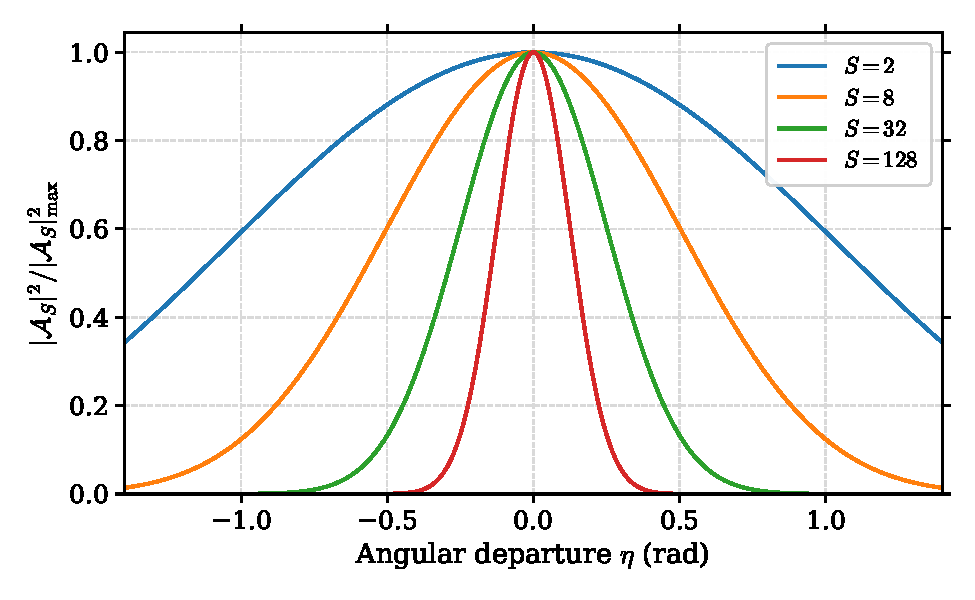
\includegraphics[width=.82\linewidth]{content/FreeElectronQuantumOptics/figures/geometry-highspin/generated/relative_angle_profiles.pdf}
 \caption{两点都位于所选大圆时，场振幅的归一化平方模随相对角偏离量 $\eta$ 的变化。这里绘制 $[\cos(\eta/2)]^{2S}$ 的非负主峰，曲线越窄代表自旋越大；纵轴只在峰值处归一为一，不代表正交位置的概率密度。}
 \label{fig:ghs-relative-profiles}
\end{figure}


为定量比较不同 $S$ 下的场振幅形状，可以构造一个\emph{场振幅权重}而不将它冒充粒子位置概率：
\begin{equation}\label{eq:ghs-field-intensity}
 \mathscr P_S(\vb n_1,\vb n_2)=\frac{|z_1-z_2|^{2S}}{Z_{d,S}},\qquad
 Z_{d,S}=\int\dd\Omega_1\dd\Omega_2\,|z_1-z_2|^{2S}.
\end{equation}
这个正函数对双球面测度归一为一。它有明确的数学意义，但属于哪种实验测量分布，必须另行给出探测模型。

把 $(z_1-z_2)^S$ 依二项式定理展开后，不同 $z^k$ 在旋转平面上的角权重互相正交。因此
\begin{equation}\label{eq:ghs-angular-norm-general}
 Z_{d,S}=\sum_{k=0}^S\binom Sk^2N_{d,k}N_{d,S-k},
\end{equation}
其中 $N_{d,k}$ 已在 \cref{eq:ghs-highest-harmonic-norm} 给出。对于四维 $N_{4,k}=2\pi^2/(k+1)$，故
\begin{align}\label{eq:ghs-angular-norm-four}
 Z_{4,S}&=(2\pi^2)^2\sum_{k=0}^S
 \frac{\binom Sk^2}{(k+1)(S-k+1)}\\
 &=(2\pi^2)^2\frac1{(S+1)^2}\binom{2S+2}{S}.\notag
\end{align}
这给出了所有非负整数 $S$ 的精确积分；其中奇数 $S$ 的数学权重依然有定义，但不对应同种玻色场的非零初级态。


有限求和可以利用二项式恒等式化简。
利用
\begin{proof}
\begin{equation*}
\frac{\binom Sk^2}{(k+1)(S-k+1)}
=\frac{\binom{S+1}{k}\binom{S+1}{k+1}}{(S+1)^2}
\end{equation*}
后，Vandermonde 卷积给出
\begin{equation*}
\sum_{k=0}^S\binom{S+1}{k}\binom{S+1}{k+1}
=\binom{2S+2}{S}.
\end{equation*}
比较 $S=0$：$Z_{4,0}=\Omega_3^2$；比较 $S=1$：$Z_{4,1}=\Omega_3^2$。这两项也可以直接将 $|z_1-z_2|^2$ 展开后利用球面角平均求出。
\end{proof}

在峰附近，$S^{d-1}$ 的角测度可按 \cref{eq:ghs-angular-coordinates} 写成局部的 $\dd^{d-2}\vb u\,\dd\varphi$ 乘上趋于 $1$ 的 Jacobian。令 $m=d-2$，平方模的高斯积分给出
\begin{align*}
 Z_{d,S}&\sim4^S(2\pi)
 \int_{\RR^m}\dd^m\vb u_1\,\ee^{-S|\vb u_1|^2/2}
 \int_{\RR^m}\dd^m\vb u_2\,\ee^{-S|\vb u_2|^2/2}
 \int_{\RR}\dd\eta\,\ee^{-S\eta^2/4}\\
 &=4^S(2\pi)\left(\frac{2\pi}{S}\right)^m
 \sqrt{\frac{4\pi}{S}}\,[1+O(S^{-1})].
\end{align*}
这说明积分的尺度为 $Z_{d,S}\asymp 4^S S^{-(d-3/2)}$。共同旋转贡献的 $2\pi$ 是整体方位零模的体积，不能再做高斯积分；否则会错误地把总方向也解释为局域化了。

\begin{figure}[htbp]
 \centering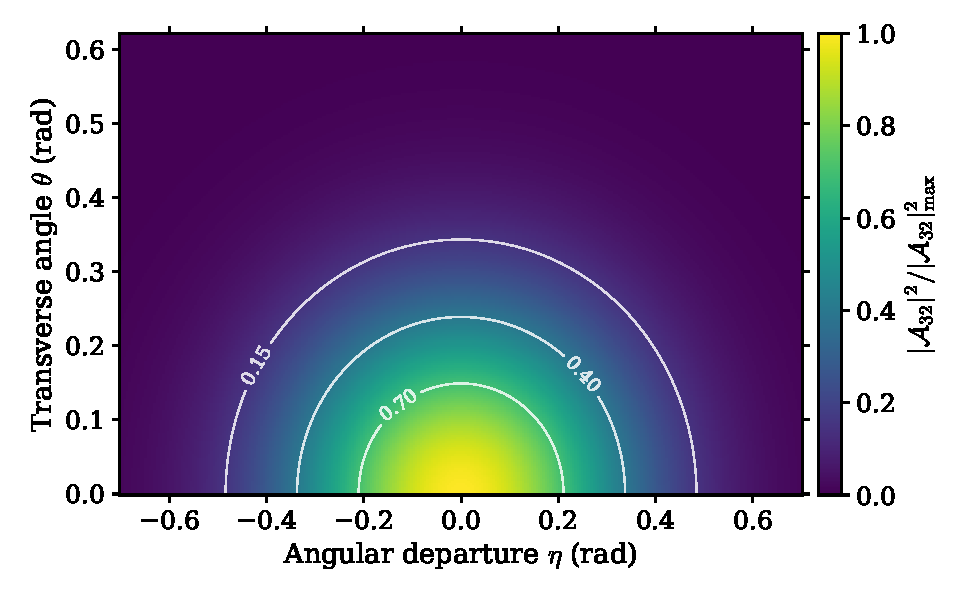
\includegraphics[width=.79\linewidth]{content/FreeElectronQuantumOptics/figures/geometry-highspin/generated/antipodal_peak_map.pdf}
 \caption{四维球面上固定第一个点于 $z_1=1$，第二个点取 $z_2=\cos\theta\,\ee^{\ii(\pi+\eta)}$。图为 $S=32$ 的精确相对峰值 $|1-z_2|^{64}/2^{64}$，并未采用高斯近似。靠近峰顶的椭圆结构对应 \cref{eq:ghs-gaussian-amplitude} 的二次型。}
 \label{fig:ghs-antipodal-map}
\end{figure}


\cref{eq:ghs-canonical-vs-field} 的谱乘子在每个 $z_1^kz_2^{S-k}$ 分量上产生 $2\sqrt{(k+\delta)(S-k+\delta)}$。如果沿着对径峰做鞍点分析，二项式展开的主要 $k$ 位于 $S/2+O(\sqrt S)$，因此
\begin{equation}\label{eq:ghs-canonical-asymptotic-multiplier}
 2\sqrt{(k+\delta)(S-k+\delta)}
 =S+2\delta-\frac{2(k-S/2)^2}{S+2\delta}
 +O\!\left(\frac{(k-S/2)^4}{S^3}\right).
\end{equation}
这里的 $k$ 是二项式和中的形式指标，复系数带有符号；在近峰复鞍点分析里不能将它的权重未经论证地当作概率分布。上述展开只解释了为什么谱乘子在局部尺度上不改变主导的 $S^{-1/2}$ 几何宽度，而没有把 \cref{eq:ghs-gaussian-amplitude} 的全部有限自旋误差项原封不动转移给正交位置密度。需要精确探测概率时，应直接计算 \cref{eq:ghs-canonical-vs-field}，而不是对场振幅简单平方。


双粒子振幅给出了自由高自旋态的空间结构，但空间集中程度本身不足以刻画态的全部信息。对其中一个粒子取偏迹，才能进一步读出模式权重与量子关联。


现在可以从另一条路线理解高自旋双粒子态：不先从 Wick 收缩出发，而是从共形对称所容许的算符表示与守恒律出发。两条路线必须描述同一组量子数。这样的交叉检验能够揭示计算中哪些结论是由一般对称性固定的，哪些只在自由高斯场里成立。


自由标量场的典型自旋二守恒流是经过共形改进的应力张量。在平直欧氏空间，令 $\varphi$ 满足运动方程 $\partial^2\varphi=0$，可取
\begin{equation}\label{eq:ghs-improved-stress}
 T_{\mu\nu}=:\!\partial_\mu\varphi\,\partial_\nu\varphi\!:
 -\frac12\delta_{\mu\nu}:\!(\partial\varphi)^2\!:
 +\xi_d(\delta_{\mu\nu}\partial^2-\partial_\mu\partial_\nu):\!\varphi^2\!: .
\end{equation}
将它对零极化向量做两次收缩，含 $\delta_{\mu\nu}$ 的项消失：
\begin{align*}
 T_{++}&\equiv\varepsilon^\mu\varepsilon^\nu T_{\mu\nu}
 =:(D_+\varphi)^2:-\xi_dD_+^2:\!\varphi^2\!:\\
 &=(1-2\xi_d):(D_+\varphi)^2:-2\xi_d:\!\varphi D_+^2\varphi\!: .
\end{align*}
把 \cref{eq:ghs-conformal-coupling,eq:ghs-spin-two-current} 代入，发现
\begin{equation}\label{eq:ghs-stress-spin-two}
 \mathcal O_2=-\frac1{\xi_d}T_{++}.
\end{equation}
因此自旋二初级算符不是随意的二导数组合，而正是自由标量应力张量的最高权分量，仅差整体归一化。


\begin{proof}
对 \cref{eq:ghs-improved-stress} 求散度，利用乘积法则与导数交换性：
\begin{align*}
\partial^\mu T_{\mu\nu}
&=:(\partial^2\varphi)\partial_\nu\varphi:
+:\!\partial^\mu\varphi\,\partial_\mu\partial_\nu\varphi\!:
-\frac12\partial_\nu:\!(\partial\varphi)^2\!:\\
&\hspace{1.5em}+\xi_d(\partial_\nu\partial^2-\partial^2\partial_\nu):\!\varphi^2\!:
=0.
\end{align*}
其中第二、第三项逐项抵消；第一项由运动方程为零。迹则为
\begin{align*}
\delta^{\mu\nu}T_{\mu\nu}
&=\left(1-\frac d2\right):\!(\partial\varphi)^2\!:
+\xi_d(d-1)\partial^2:\!\varphi^2\!:\\
&=\bigl[-\delta+2\xi_d(d-1)\bigr]:\!(\partial\varphi)^2\!:=0,
\end{align*}
这里用了 $\partial^2:\!\varphi^2\!:=2:\!(\partial\varphi)^2\!:$。可见恢复含度规的张量项以后，无迹性和守恒性才同时正确。
\end{proof}

\subsection{总自旋、应力张量与模式划分}

一个旋转平面的共同变换 $z_i\mapsto\ee^{\ii\alpha}z_i$ 将振幅变为 $\ee^{\ii S\alpha}\mathcal A_S$。所以 $S$ 是整个双粒子态的角动量最高权，而不是说每个粒子各自具有角动量 $S$。具体的 Fock 展开包含
\begin{equation}\label{eq:ghs-two-mode-fock}
 |S\rangle=\frac1{\sqrt{\mathcal N_S}}
 \sum_{k=0}^S c_kF_kF_{S-k}
 b_k^\dagger b_{S-k}^\dagger|0\rangle.
\end{equation}
各项的单粒子球谐阶数为 $(k,S-k)$，总能量始终是 $(k+\delta)+(S-k+\delta)=S+2\delta$。高自旋态不是两个各自都处在 $\ell=S$ 的粒子，而是许多能量划分共享同一总角动量的相干叠加。

在四维自旋二情形，这一点可以直接看清：按照 $F_0=1/(2\pi)$、$F_1=1/\pi$、$F_2=4/\pi$ 的归一化，有
\begin{equation}\label{eq:ghs-spin-two-fock}
 |\mathcal O_2\rangle=\frac4{\pi^2}
 \left(b_0^\dagger b_2^\dagger-(b_1^\dagger)^2\right)|0\rangle,
 \qquad \|\mathcal O_2\|^2=\frac{48}{\pi^4}.
\end{equation}
其中两个独立的粒子数模式 $(0,2)$ 与 $(1,1)$ 之间的相对负号，恰好是特殊共形初级条件选出的相干结构。若只看能量谱或者单粒子角动量，无法推断这个负号。


几何变换 \cref{eq:ghs-weyl-cylinder} 和共形理论的态—算符对应不局限于自由场。一个一般幺正共形场论中的自旋 $S$ 初级算符仍然具有标度维数 $\Delta_{S}$，其圆柱激发能量为 $\hbar c\Delta_S/R$；对称性也依旧限制二点与三点函数的空间结构。但下列性质依赖自由场的具体动力学：

一是传播子恰好等于 $C_d|x|^{-2\delta}$ 且所有高阶函数可依 Wick 定理分解。二是局域双线性含恰好两个自由振子量子。三是对每个偶数 $S\ge2$ 都有守恒流与精确维数 $S+d-2$。一旦发生相互作用，高自旋流一般不再守恒，算符维数可能变为 $\Delta_S=d-2+S+\gamma_S$，其中 $\gamma_S$ 是相应算符的反常维数；但应力张量若存在且守恒，其自旋二维数仍由 Ward 恒等式保护。

四是 $\mathcal A_S\propto(z_1-z_2)^S$ 的简洁多项式依赖自由 Wick 收缩与此处选定的两个场插入。相互作用理论中的三点函数会受到所选算符及其归一化影响；不应仅凭总自旋便把自由场的全部空间概率结构外推到一般介质、散射粒子或其他非共形体系。


径向量子化把原本看似独立的三件事连到了一起。第一，尺度变换成为圆柱时间平移，产生谱 $\omega_\ell=\ell+\delta$。第二，特殊共形生成元从同一能量简并子空间中选出初级态，其系数满足 \cref{eq:ghs-primary-recurrence}。第三，用自由场传播子把这个初级态投影到两个场插入上，有限和恰好收束成 \cref{eq:ghs-amplitude-exact}。大自旋时，后一个结果的模集中在同一大圆上的对径构型；而其相位携带共同旋转的最高权 $S$。

这些结论构成一个可直接复算的自由场专题，而非关于真实双粒子经典轨道的主张。若要讨论测量所得的相对位置分布，必须进一步使用 \cref{eq:ghs-canonical-vs-field} 或具体探测器的测量算符。


\subsection{单体约化谱与模式熵}

双粒子态还包含另一种可以精确计算的信息：当其中一个粒子不被观测时，剩余粒子的约化态是什么。它应从归一化的对称 Fock 系数求得，而不能由空间峰的形状直接推断。


大自旋时球面场振幅沿对径构型集中，但这种空间相关并没有直接告诉我们两个量子的角动量如何分配。由于前面已经把局域算符准确写成了双振子态，现在可以不作近似地对其中一个粒子求偏迹，得到单体密度算符和谱。这个计算也提供一条独立于坐标空间鞍点法的高自旋渐近分析。


\begin{proposition}[单体约化谱]
在正交模式 $b_k^\dagger$ 下，\cref{eq:ghs-two-mode-fock} 是一个对称双粒子态。其一阶关联矩阵定义为
\begin{equation}\label{eq:ghs-one-body-density-definition}
 (\rho_1)_{jk}=\frac12\langle S|b_k^\dagger b_j|S\rangle.
\end{equation}
因总粒子数为 $2$，$\Tr\rho_1=1$。每个 Fock 分量都满足 $k+(S-k)=S$，故一阶关联矩阵在这一模式基底上对角：
\begin{equation}\label{eq:ghs-one-body-spectrum-general}
 \rho_1=\sum_{k=0}^S p_k|k\rangle\langle k|,\qquad
 p_k=\frac{2|B_k|^2}{\mathcal N_S}
 =\frac{(\delta)_S^2}{(2\delta+S-1)_S}
 \frac{\binom Sk}{(\delta)_k(\delta)_{S-k}}.
\end{equation}
这里 $|k\rangle=b_k^\dagger|0\rangle$ 是一个归一化单粒子模式。Vandermonde 恒等式给出 $\sum_kp_k=1$，又有 $p_k=p_{S-k}$，故平均单体球谐阶数严格等于 $S/2$。

该分布描述的是在对称双粒子态中随机选取一个粒子时得到的模式占据权重。由于粒子不可辨认，$\rho_1$ 的熵属于\emph{单体约化谱的熵}；不能不加区分地解释成两个可独立寻址实验室子系统之间的可操作纠缠熵。
\end{proposition}

\begin{proof}
记 $|\widetilde S\rangle=\sum_kB_kb_k^\dagger b_{S-k}^\dagger|0\rangle$。由玻色对易关系
\begin{equation*}
b_j|\widetilde S\rangle
=\sum_kB_k(\delta_{jk}b_{S-k}^\dagger+\delta_{j,S-k}b_k^\dagger)|0\rangle
=2B_jb_{S-j}^\dagger|0\rangle
\end{equation*}
（这里用了偶数 $S$ 的 $B_j=B_{S-j}$）。因此
\begin{align*}
\langle\widetilde S|b_k^\dagger b_j|\widetilde S\rangle
&=4B_k^*B_j\langle0|b_{S-k}b_{S-j}^\dagger|0\rangle\\
&=4|B_j|^2\delta_{kj}.
\end{align*}
除以 $2\mathcal N_S$ 就得到 \cref{eq:ghs-one-body-spectrum-general}。这一推导自动处理了 $k=S/2$ 两个粒子位于同一模式的情形，不需要人为增加或删除对称因子。
\end{proof}

\begin{example}[四维模式谱与超几何分布]
在四维 $\delta=1$，使用 $(1)_k=k!$，上式化为
\begin{equation}\label{eq:ghs-hypergeometric-mode-distribution}
 p_k=\frac{\binom Sk^2}{\binom{2S}{S}},\qquad
 k=0,1,\ldots,S,\qquad S\in2\NN_0.
\end{equation}
分母由 Vandermonde 恒等式 $\sum_{k=0}^S\binom Sk^2=\binom{2S}{S}$ 确定。这个分布恰好等于从 $2S$ 个物体中不放回抽取 $S$ 个、其中 $S$ 个属于某一类时所得到的超几何分布。因此可以直接计算它的前两阶矩：
\begin{equation}\label{eq:ghs-mode-variance}
 \mathbb E(k)=\frac S2,\qquad
 \operatorname{Var}(k)=\frac{S^2}{4(2S-1)},\qquad S\ge2.
\end{equation}
例如 $S=2$ 时，$p_0=p_2=1/6$、$p_1=2/3$，与 \cref{eq:ghs-spin-two-fock} 的粒子数配比完全一致。$S=0$ 是确定的单模式纯态，方差直接取零，无需使用右侧分母 $2S-1$ 的公式。
\end{example}

当 $S\to\infty$，中心极限定理或直接对阶乘使用 Stirling 展开可得局部极限定理
\begin{equation}\label{eq:ghs-mode-central-limit}
 p_k=\frac{2}{\sqrt{\pi S}}
 \exp\!\left[-\frac{4(k-S/2)^2}{S}\right]
 \left[1+O(S^{-1/2})\right],
 \quad |k-S/2|=O(\sqrt S).
\end{equation}
误差对于固定缩放变量 $(k-S/2)/\sqrt S$ 的有界集合一致；若 $k$ 接近 $0$ 或 $S$，必须使用完整的组合数而不能继续套用高斯近似。

\begin{figure}[htbp]
 \centering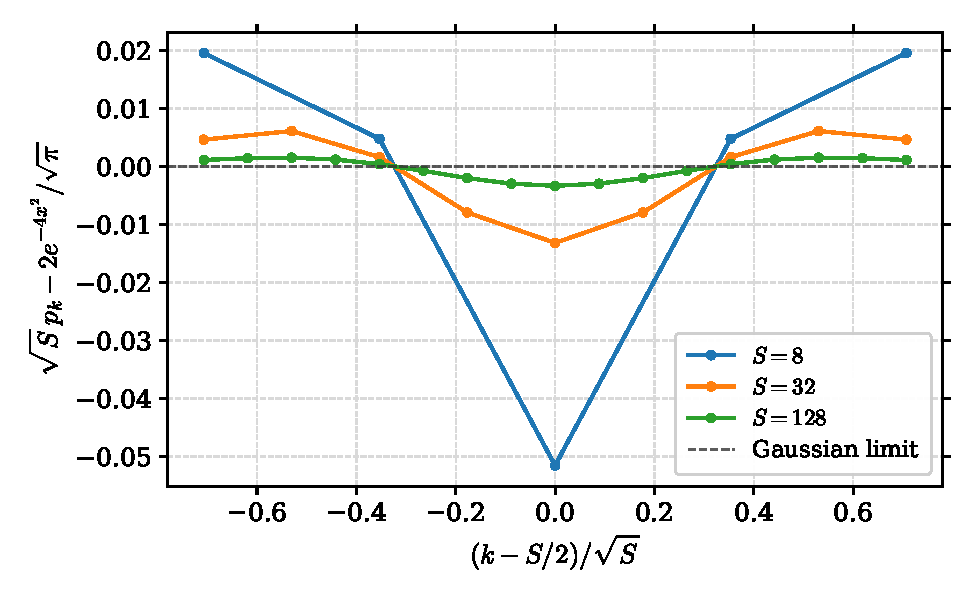
\includegraphics[width=.8\linewidth]{content/FreeElectronQuantumOptics/figures/geometry-highspin/generated/mode_occupation.pdf}
 \caption{四维双粒子初级态的模式概率相对极限高斯的直接误差。图仅保留主峰区间 $|x|\le0.75$，避免近零尾部压缩尺度；不同自旋的离散误差清楚分离，而不是将近乎重合的概率密度反复叠加。这里 $x=(k-S/2)/\sqrt S$，$p_k$ 是正交 Fock 模式的概率。}
 \label{fig:ghs-mode-occupation}
\end{figure}


一粒子约化密度算符的 冯诺依曼熵在这一对角基中就是离散 香农熵：
\begin{equation}\label{eq:ghs-onebody-entropy}
 \mathsf S_1(S)=-\Tr(\rho_1\log\rho_1)
 =-\sum_{k=0}^S p_k\log p_k.
\end{equation}
对有限偶数 $S$，\cref{eq:ghs-hypergeometric-mode-distribution} 给出不含任何未知系数的精确有限和。大自旋时，离散高斯的方差为 $S/8+O(1)$，因此
\begin{equation}\label{eq:ghs-onebody-entropy-asymptotic}
 \mathsf S_1(S)=\frac12\log\!\left(\frac{\pi\ee S}{4}\right)+o(1),
 \qquad S\to\infty,\ S\text{ 为偶数}.
\end{equation}
熵只按 $\frac12\log S$ 缓慢增长，而不是正比于 $S$。这与模式分布集中在 $k=S/2+O(\sqrt S)$ 的事实一致：有效参与的单体模式数约为 $\sqrt S$，因而熵的主阶是其对数。


因为 $\rho_1$ 在最高权球谐模式下对角，单粒子角密度可以精确写成
\begin{equation}\label{eq:ghs-onebody-angular-density}
 \rho_1(\vb n,\vb n)=\sum_{k=0}^S p_k|y_k(\vb n)|^2
 =\sum_{k=0}^S p_k\frac{|z|^{2k}}{N_{d,k}}.
\end{equation}
它对球面测度归一为 $1$，并且不依赖 $z$ 的相位。也就是说，一个粒子的单体测量无法挑出大圆上的某一个绝对方位；对径关系蕴藏在联合测量的关联中。

四维时 $N_{4,k}=\Omega_3/(k+1)$。在大圆上 $|z|=1$，由 $\mathbb E(k)=S/2$ 得到一个精确峰值公式
\begin{equation}\label{eq:ghs-onebody-angular-maximum}
 \rho_1(\vb n,\vb n)\big|_{|z|=1}
 =\frac{1}{\Omega_3}\sum_k(k+1)p_k
 =\frac{S/2+1}{2\pi^2}.
\end{equation}
对于离开大圆的法向距离 $|\vb u|=\theta+O(\theta^3)$，$|z|^{2k}=(1-|\vb u|^2)^k$。典型 $k\simeq S/2$，所以单体密度的横向包络是 $\exp(-S|\vb u|^2/2)$，宽度同样为 $O(S^{-1/2})$。单体密度沿整条大圆均匀分布，联合振幅进一步要求第二粒子位于对径附近。两个结论相容，但不可混为一谈。


单体谱给出了高自旋态的精确概率分布。只有在有限自旋结果已经归一化后，才能求其局部极限及误差，而不是仅凭一条形似高斯的曲线猜测渐近规律。


自由场的长程结构可以从两个互补的角度观察。一种是将双场矩阵元限制在球面的大圆上，看两点偏离对径时振幅怎样衰减；另一种是把严格归一的 Fock 态对一个量子求偏迹，看单粒子角动量模式怎样分布。二者分别使用不同的数学测度，不能将其密度直接相等，但它们的有限自旋修正都可以从精确公式而不是高斯猜测出发计算。


\subsection{圆周矩与有限自旋渐近}

\begin{definition}[大圆上的归一化场权重]
在 \cref{eq:ghs-angular-coordinates} 中施加 $|z_1|=|z_2|=1$，并设 $\varphi_2-\varphi_1=\pi+\eta$，$-\pi\le\eta\le\pi$。沿这一一维几何子空间，场振幅平方的相对形状为
\begin{equation}\label{eq:ghs-circle-antipodal-profile}
 \frac{|z_1-z_2|^{2S}}{4^S}
 =\cos^{2S}(\eta/2).
\end{equation}
这一限制不等同于从完整 $S^{d-1}\times S^{d-1}$ 权重中对概率为零的子流形无条件求条件分布。现在独立给大圆赋予标准角测度 $\dd\eta$，再将限制后的权重重新归一，定义圆周角分布
\begin{equation}\label{eq:ghs-circle-normalized-density}
 q_S(\eta)=\frac{4^S}{2\pi\binom{2S}{S}}\cos^{2S}(\eta/2),
 \qquad\int_{-\pi}^{\pi}q_S(\eta)\,\dd\eta=1.
\end{equation}
对任意非负整数 $S$，它都是数学上严格的概率密度；只有偶数 $S$ 才能同时对应前面同种自由实标量的非零双线性初级态。
\end{definition}

\begin{proof}
利用 $2\cos(\eta/2)=\ee^{\ii\eta/2}+\ee^{-\ii\eta/2}$，二项式展开得到
\begin{align*}
4^S\cos^{2S}(\eta/2)
&=(\ee^{\ii\eta/2}+\ee^{-\ii\eta/2})^{2S}\\
&=\sum_{j=0}^{2S}\binom{2S}{j}\ee^{\ii(j-S)\eta}
=\sum_{m=-S}^S\binom{2S}{S+m}\ee^{\ii m\eta}.
\end{align*}
角积分只保留 $m=0$ 的常数项，因此
\begin{equation*}
\int_{-\pi}^{\pi}\cos^{2S}(\eta/2)\,\dd\eta
=\frac{2\pi}{4^S}\binom{2S}{S}.
\end{equation*}
\end{proof}

\begin{proposition}[圆周 Fourier 矩与集中尺度]
因为 $q_S$ 是一个非负三角多项式，任意整数谐波的期望均可从上一段展开直接读取：
\begin{equation}\label{eq:ghs-circle-fourier-moments}
 \langle\ee^{\ii m\eta}\rangle_{q_S}
 =\begin{cases}
 \displaystyle\frac{\binom{2S}{S+m}}{\binom{2S}{S}},& |m|\le S,\\[6pt]
 0,& |m|>S.
 \end{cases}
\end{equation}
所有正弦矩均为零。特别地，一阶余弦矩为 $S/(S+1)$，所以圆周统计中不依赖角坐标切口的集中尺度可以定义为
\begin{equation}\label{eq:ghs-circle-circular-variance}
 V_{\rm circ}(S)=1-\langle\cos\eta\rangle_{q_S}
 =\frac1{S+1}.
\end{equation}
这个公式对有限 $S$ 也精确成立。大自旋时，由 $1-\cos\eta=\eta^2/2+O(\eta^4)$，可知局部欧氏角方差为 $2/S+O(S^{-2})$，与 \cref{eq:ghs-peak-variances} 的鞍点估计一致。
\end{proposition}

固定非负整数 $m$，Fourier 矩还可以写成有限连乘积
\begin{equation}\label{eq:ghs-circle-moment-product}
 \langle\ee^{\ii m\eta}\rangle_{q_S}
 =\prod_{j=1}^{m}\frac{S-j+1}{S+j},\qquad m\le S.
\end{equation}
若 $m$ 与 $S$ 一同增大，直接将对数展开，
\begin{align*}
 \log\langle\ee^{\ii m\eta}\rangle_{q_S}
 &=\sum_{j=1}^m\left[\log\left(1-\frac{j-1}{S}\right)
 -\log\left(1+\frac{j}{S}\right)\right]\\
 &=-\frac{m^2}{S}+O\!\left(\frac{m^2}{S^2}+\frac{m^4}{S^3}\right),
\end{align*}
在 $m=O(\sqrt S)$ 的范围内，主导结果是 $\ee^{-m^2/S}$。这正是方差为 $2/S$ 的局部高斯分布之特征函数；因而对径峰的角宽度也能从 Fourier 矩而非仅从峰顶 Taylor 级数得到。


\begin{proposition}[圆周峰的第一项形状修正]
大圆上的精确分布不只是近似高斯；由于它是单个余弦幂，还能算出高斯极限之后的第一项形状修正。令 $x=\sqrt{S/2}\,\eta$，把圆周密度相应写为 $q_S^{(x)}(x)=\sqrt{2/S}\,q_S(x\sqrt{2/S})$。在固定有界 $x$ 的极限中，
\begin{equation}\label{eq:ghs-circle-edgeworth-correction}
 q_S^{(x)}(x)
 =\frac{\ee^{-x^2/2}}{\sqrt{2\pi}}
 \left[1+\frac1S\left(\frac18-\frac{x^4}{24}\right)
 +O(S^{-2})\right].
\end{equation}
修正系数的 $x^4$ 项让峰顶附近比高斯略高、肩部略低。它的高斯平均严格为零，因为标准正态的四阶矩等于 $3$；所以展开在 $1/S$ 阶仍然保持归一化。
\end{proposition}

\begin{proof}
对 $|x|=O(1)$，设 $\eta=\sqrt{2/S}\,x$。由 $\log\cos y=-y^2/2-y^4/12+O(y^6)$，
\begin{equation*}
2S\log\cos(\eta/2)
=-\frac{x^2}{2}-\frac{x^4}{24S}+O(S^{-2}).
\end{equation*}
另一方面，中心二项式的 Stirling 展开是
\begin{equation*}
\log\binom{2S}{S}
=S\log4-\frac12\log(\pi S)-\frac1{8S}+O(S^{-3}).
\end{equation*}
将两式代入 \cref{eq:ghs-circle-normalized-density}，并加入测度变化 $\dd\eta=\sqrt{2/S}\,\dd x$，整理指数得到
\begin{equation*}
\log q_S^{(x)}(x)=-\frac12\log(2\pi)-\frac{x^2}2
+\frac1S\left(\frac18-\frac{x^4}{24}\right)+O(S^{-2}).
\end{equation*}
指数化以后即为 \cref{eq:ghs-circle-edgeworth-correction}。
\end{proof}

\subsection{一般维数极限与 Rényi 熵}

已有精确模式分布
\begin{equation}\label{eq:ghs-all-d-onebody-p}
 p_k=\frac{(\delta)_S^2}{(2\delta+S-1)_S}
 \frac{\binom Sk}{(\delta)_k(\delta)_{S-k}},
 \qquad\delta=\frac{d-2}{2}>0.
\end{equation}
为了分析不同维数下的高自旋极限，忽略只依赖 $S$ 的整体因子，将其写为
\begin{equation*}
 p_k\propto\frac1{\Gamma(k+1)\Gamma(S-k+1)
 \Gamma(k+\delta)\Gamma(S-k+\delta)}.
\end{equation*}
对数关于 $k=S/2$ 对称，其一阶导数必然为零。设 $k=S/2+x\sqrt S$，固定 $x$，利用 $\log\Gamma$ 的导数渐近展开可得
\begin{equation}\label{eq:ghs-all-d-local-gaussian}
 \sqrt S\,p_{\lfloor S/2+x\sqrt S\rfloor}
 \longrightarrow\frac2{\sqrt\pi}\ee^{-4x^2},
 \qquad S\to\infty,
\end{equation}
在固定 $x$ 的紧区间上一致成立。因此任意固定 $d>2$ 的主导分布均为同一个高斯核，
\begin{equation}\label{eq:ghs-all-d-asymptotic-variance}
 \operatorname{Var}(k)=\frac S8+O(1),
 \qquad\mathbb E(k)=S/2.
\end{equation}
维数 $d$ 改变有限自旋权重和次领先修正，但不改变中央涨落的 $\sqrt S$ 尺度。这里的极限是先固定 $d$ 再令 $S\to\infty$；如果 $d$ 同时与 $S$ 增大，就不能照搬 \cref{eq:ghs-all-d-local-gaussian}。


\begin{proof}
设 $f_S(k)=\log p_k+\text{与 $k$ 无关的常数}$，则
\begin{align*}
f_S'(k)
&=-\psi(k+1)+\psi(S-k+1)
-\psi(k+\delta)+\psi(S-k+\delta),\\
f_S''(k)
&=-\psi_1(k+1)-\psi_1(S-k+1)
-\psi_1(k+\delta)-\psi_1(S-k+\delta),
\end{align*}
其中 $\psi$ 和 $\psi_1$ 分别是二伽马函数及其导数。代入 $k=S/2$，利用 $\psi_1(y)=y^{-1}+O(y^{-2})$，得到
\begin{equation*}
f_S'(S/2)=0,\qquad f_S''(S/2)=-\frac8S+O(S^{-2}).
\end{equation*}
对 $k-S/2=x\sqrt S$ 作 Taylor 展开，奇次项因左右对称而消失，故
\begin{equation*}
f_S(S/2+x\sqrt S)-f_S(S/2)
=-4x^2+O(S^{-1})
\end{equation*}
对有界 $x$ 一致成立。归一化由 $\sum_kp_k=1$ 和离散和的 Riemann 逼近给出 $p_{S/2}\sim 2/\sqrt{\pi S}$，于是得到 \cref{eq:ghs-all-d-local-gaussian}。尾部衰减可从 $p_{k+1}/p_k$ 的确切连乘结构控制，保证二阶矩不会由远尾主导。
\end{proof}

一般 $d$ 中的单体约化谱完全由 $p_k$ 给出。对 $q>0$ 且 $q\neq1$，定义阶数为 $q$ 的 Rényi 熵
\begin{equation}\label{eq:ghs-renyi-definition}
 H_q(S)=\frac1{1-q}\log\Tr\rho_1^q
 =\frac1{1-q}\log\sum_{k=0}^S p_k^q.
\end{equation}
当 $q\to1$ 时连续恢复 \cref{eq:ghs-onebody-entropy} 的 冯诺依曼熵。对任意固定 $q>0$ 和任意固定维数 $d>2$，将 \cref{eq:ghs-all-d-local-gaussian} 的离散高斯代入，并把求和转成积分：
\begin{align*}
 \sum_{k=0}^S p_k^q
 &\sim \sqrt S\left(\frac2{\sqrt{\pi S}}\right)^q
 \int_{-\infty}^{\infty}\ee^{-4qx^2}\,\dd x\\
 &=q^{-1/2}\left(\frac2{\sqrt{\pi S}}\right)^{q-1}.
\end{align*}
由此得到
\begin{equation}\label{eq:ghs-renyi-asymptotic}
 H_q(S)=\frac12\log\left(\frac{\pi S}{4}\right)
 +\frac{\log q}{2(q-1)}+o(1).
\end{equation}
特别地，$q\to1$ 给出 $H_1=\frac12\log(\pi\ee S/4)+o(1)$；$q=2$ 则控制纯度
\begin{equation}\label{eq:ghs-onebody-purity-asymptotic}
 \Tr\rho_1^2=\sum_kp_k^2
 =\sqrt{\frac2{\pi S}}\,[1+o(1)].
\end{equation}
二阶 Rényi 熵的指数 $\ee^{H_2}=1/\Tr\rho_1^2$ 可视为参与模式数的一个标准定义，其主阶正比于 $\sqrt S$，而不是 $S$。这种增长刻画单体模式占据谱的展开，但对于不可辨认玻色子，仍不应不加说明地等同于两个可独立操作实验粒子的纠缠资源。


\begin{proposition}[四维单体熵的有限自旋修正]
主导的 $\tfrac12\log S$ 只告诉我们参与模式数的数量级，而低自旋时的偏差还需要从精确组合数计算。四维中的 $p_k=\binom Sk^2/\binom{2S}{S}$ 允许进一步把熵计算到 $S^{-1}$ 阶。结果是
\begin{align}\label{eq:ghs-entropy-next-order}
 H_1(S)&=\frac12\log\left(\frac{\pi\ee S}{4}\right)
 +\frac1{4S}+O(S^{-2}),\\
 H_2(S)&=\frac12\log\left(\frac{\pi S}{2}\right)
 +\frac5{16S}+O(S^{-2}).\notag
\end{align}
因此两个熵靠近高斯极限的速率虽然同为 $S^{-1}$，但系数不同。下面把这一差别真正从 Stirling 展开算出，而不只用数值拟合猜测系数。
\end{proposition}

\begin{proof}
令 $x=(k-S/2)/\sqrt S$，并暂时固定有界的 $x$。对 $\log\Gamma$ 使用含 $1/(12n)$ 的 Stirling 展开，分别计算两个分子组合数及分母，得到
\begin{align*}
\log p_k
&=\log\frac2{\sqrt{\pi S}}-4x^2+\frac{a(x)}S
+O\left(S^{-2}(1+|x|^6)\right),\\
a(x)&=-\frac83x^4+4x^2-\frac38.
\end{align*}
主导高斯密度为 $q_4(x)=2\ee^{-4x^2}/\sqrt\pi$。其偶次矩为
\begin{equation*}
\langle x^2\rangle_{q_4}=\frac18,\qquad
\langle x^4\rangle_{q_4}=\frac3{64},\qquad
\langle a(x)\rangle_{q_4}=0.
\end{equation*}
取负平均对数，由精确方差公式 \cref{eq:ghs-mode-variance}，
\begin{align*}
H_1(S)
&=\log\frac{\sqrt{\pi S}}2+4\langle x^2\rangle_{p}
-\frac1S\langle a(x)\rangle_{p}+O(S^{-2})\\
&=\log\frac{\sqrt{\pi S}}2
+\frac{S}{2S-1}+O(S^{-2})\\
&=\frac12\log\frac{\pi\ee S}{4}
+\frac1{4S}+O(S^{-2}).
\end{align*}
这里 $\langle a\rangle_p=O(S^{-1})$，所以它乘以前面的 $1/S$ 后只影响 $S^{-2}$ 阶。

对于纯度，平方 $p_k$ 会把主导高斯改成 $q_8(x)=\sqrt{8/\pi}\ee^{-8x^2}$。新的矩为 $\langle x^2\rangle_{q_8}=1/16$、$\langle x^4\rangle_{q_8}=3/256$，于是
\begin{equation*}
\langle a(x)\rangle_{q_8}
=-\frac83\frac3{256}+4\frac1{16}-\frac38
=-\frac5{32}.
\end{equation*}
将离散求和转为局部高斯积分，得到
\begin{align*}
\Tr\rho_1^2
&=\sqrt{\frac2{\pi S}}
\left[1+\frac2S\langle a(x)\rangle_{q_8}
+O(S^{-2})\right]\\
&=\sqrt{\frac2{\pi S}}
\left[1-\frac5{16S}+O(S^{-2})\right].
\end{align*}
再取负对数便得到 \cref{eq:ghs-entropy-next-order} 的第二行。由于精确分布的中心外尾部按指数衰减，可以在控制尾部后逐项积分；离散格点的 Poisson 求和修正对这些光滑高斯核指数小于任何固定 $S^{-n}$。
\end{proof}

\begin{figure}[htbp]
 \centering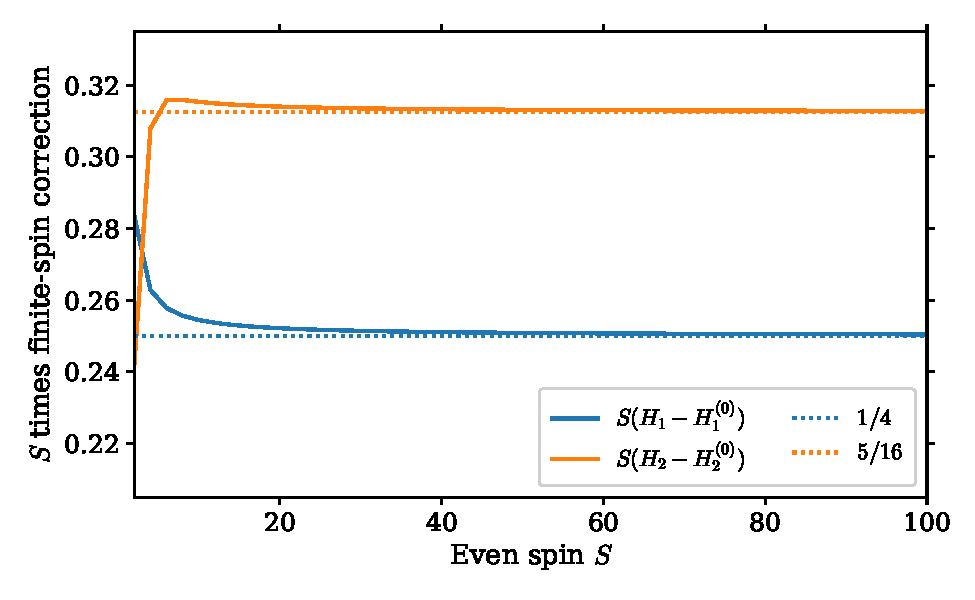
\includegraphics[width=.82\linewidth]{content/FreeElectronQuantumOptics/figures/geometry-highspin/generated/renyi_entropy_scaling.pdf}
 \caption{四维自由标量的两类单体熵相对高斯首阶的偏差乘以自旋 $S$。精确求和结果趋近于解析修正系数 $1/4$ 和 $5/16$；相比在同一坐标上绘制几乎重叠的熵曲线，这种差分呈现能直接检验下一阶渐近展开。}
 \label{fig:ghs-renyi-entropy}
\end{figure}


对于 $d=4$、$S=2$，模式分布为 $p=(1/6,2/3,1/6)$，它与连续高斯有明显差别。由 \cref{eq:ghs-renyi-definition}，
\begin{equation}\label{eq:ghs-spin-two-renyi}
 H_1(2)=\log3-\frac13\log2,\qquad
 H_2(2)=\log2.
\end{equation}
真正的两端分量各自只有 $1/6$，中间分量却有 $2/3$，说明最初几个偶数自旋的态仍是少数离散 Fock 模式的干涉，而不是经典角变量的窄波包。所有高斯、熵和 Fourier 近似都应在明确的 $S\to\infty$ 区间使用。

\begin{figure}[htbp]
 \centering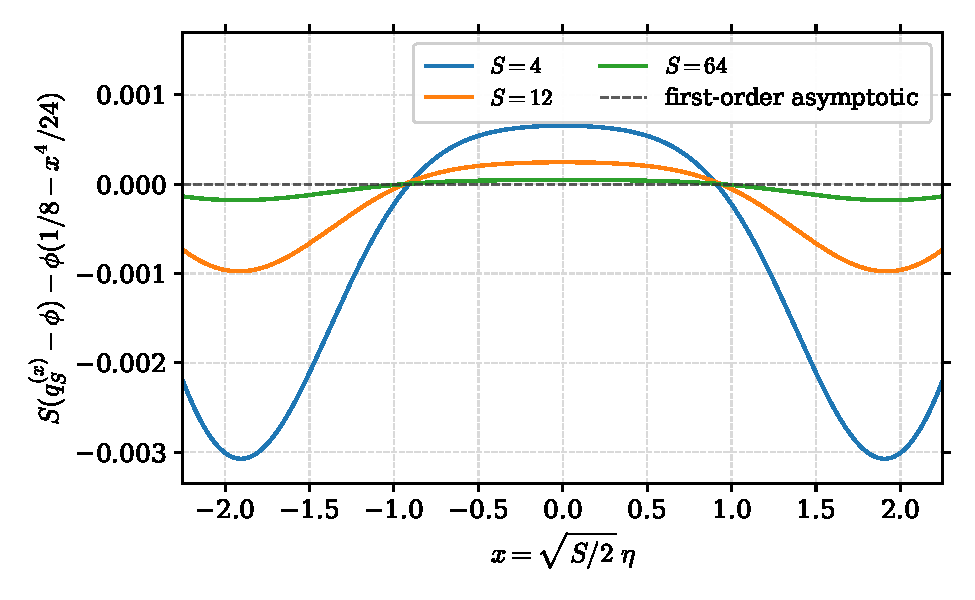
\includegraphics[width=.80\linewidth]{content/FreeElectronQuantumOptics/figures/geometry-highspin/generated/circle_fourier_profiles.pdf}
 \caption{对大圆角密度去除高斯首项以及 $1/S$ 阶解析修正后，剩余误差乘以 $S$。它直接展示首个非高斯渐近公式在有限自旋下的精度；虚线零基线对应已保留的渐近阶，横轴限定在主峰及肩部。}
 \label{fig:ghs-circle-fourier}
\end{figure}

\section{混合标量双线性与一般自旋关联}

这一推导还表明：所谓“守恒”并不是任意把散度设成零，而是表示论中某个后裔与物理 Hilbert 空间脱耦。自由标量的双线性流满足 $\Delta_S=S+d-2$，因而恰好处在这一边界；一般相互作用使 $\Delta_S$ 增大时，原来被模掉的后裔重新取得正范数。


前述自由双粒子态的维数 $\Delta_S=d-2+S$ 饱和幺正界。要分清这种守恒性与一般初级条件，可让两种标量具有独立维数，并重新求导数递推与 Wick 范数。由此得到的双线性算符通常不守恒，却仍然是严格的共形初级算符，而且它的归一化和三点耦合可以完全求出。


\subsection{可区分标量的初级系数与范数}

考虑 $d>2$ 维单位欧氏共形场论中的两种相互正交的标量初级算符 $A$ 和 $B$，维数为 $\Delta_A,\Delta_B\ge(d-2)/2$，选二点函数的规范化为
\begin{equation}\label{eq:ghs-r4-generalized-free-two-points}
 \langle A(x)A(0)\rangle=(x^2)^{-\Delta_A},\qquad
 \langle B(x)B(0)\rangle=(x^2)^{-\Delta_B},\qquad
 \langle A(x)B(0)\rangle=0.
\end{equation}
要求它们在所讨论的扇区中满足广义自由的高点关联函数规则：所有偶数点函数是二点函数配对之和，奇数点函数为零。这个假设不要求 $A,B$ 满足局域自由波动方程，且一般不存在一个具有通常二阶动力学的局域基本作用量。它只是精确定义了一套可用来比较任意维数与任意标度维数的双粒子 Hilbert 空间。广义自由理论的完整算符乘积数据还可用共形谐分析得到，参见 \cite{ghs-karateev-harmonic}。对于真正相互作用的共形场论，后面的 Wick 范数和三点系数不能不加检查地沿用。

径向量子化中，$A(0)|0\rangle$ 和 $B(0)|0\rangle$ 是不同的一粒子初级态。令复零向量 $z^\mu$ 满足 $z^2=0$，并记 $P_z=z^\mu P_\mu$。其 $k$ 级最高权后裔为 $P_z^k|A\rangle$，维数 $\Delta_A+k$。由于 $P_z$ 与自身对易，所有高阶导数可用一个对称无迹极化多项式编码。两个粒子的总维数为 $\Delta_A+\Delta_B+S$ 时，既有一座总导数后裔塔，也有一个去除了总导数的真正初级态。区别它们的条件是特殊共形生成元的湮灭关系。


取
\begin{equation}\label{eq:ghs-r4-mixed-bilinear-def}
 [AB]_S(x,z)=\sum_{k=0}^S c_k:
 (z\cdot\partial)^k A(x)\,(z\cdot\partial)^{S-k}B(x):,
 \qquad S\in\NN_0.
\end{equation}
这两个场是可区分的，故不存在 $k\leftrightarrow S-k$ 的交换化简。由标量初级的特殊共形变换式，可沿用 \cref{eq:ghs-K-derivative} 的计算，只需把自由场维数 $\delta$ 换成各自的 $\Delta_A$ 或 $\Delta_B$。在选定的复零方向上，降低一个导数的系数分别为 $4k(\Delta_A+k-1)$ 和 $4k(\Delta_B+k-1)$。因此两种降低途径必须相消：
\begin{equation}\label{eq:ghs-r4-mixed-recurrence}
 (j+1)(\Delta_A+j)c_{j+1}
 +(S-j)(\Delta_B+S-j-1)c_j=0,
 \quad j=0,\ldots,S-1.
\end{equation}
取 $c_0=1$，逐次消去 $c_1,\ldots,c_S$，得到
\begin{equation}\label{eq:ghs-r4-mixed-primary-coefficients}
 c_k=(-1)^k\binom Sk\frac{(\Delta_B)_S}
 {(\Delta_A)_k(\Delta_B)_{S-k}},
 \qquad(a)_n\equiv\frac{\Gamma(a+n)}{\Gamma(a)}.
\end{equation}
这条结论对任意整数 $d>2$、任意满足标量幺正性界的维数和任意非负整数自旋成立。特别地，初级维数为
\begin{equation}\label{eq:ghs-r4-mixed-dimension}
 \Delta_{[AB]_S}=\Delta_A+\Delta_B+S,
 \qquad\tau_{[AB]_S}=\Delta_A+\Delta_B.
\end{equation}
它不再一般等于 $S+d-2$。两个标量的维数越高，双线性初级态离守恒流的短表示界就越远。


把初级条件写成相邻系数的递推关系后，可以连乘求解。
先把 \cref{eq:ghs-r4-mixed-recurrence} 逐项改写为
\begin{align*}
 \frac{c_{j+1}}{c_j}
 &=-\frac{S-j}{j+1}\frac{\Delta_B+S-j-1}{\Delta_A+j},\\
 c_k&=(-1)^k\prod_{j=0}^{k-1}\frac{S-j}{j+1}
 \prod_{j=0}^{k-1}\frac{\Delta_B+S-j-1}{\Delta_A+j}\\
 &=(-1)^k\frac{S!}{k!(S-k)!}
 \frac{\Gamma(\Delta_B+S)}{\Gamma(\Delta_B+S-k)}
 \frac{\Gamma(\Delta_A)}{\Gamma(\Delta_A+k)}.
\end{align*}
现在乘除以 $\Gamma(\Delta_B)$，便恢复 \cref{eq:ghs-r4-mixed-primary-coefficients}。$S=1$ 时得到 $[AB]_1= A(z\cdot\partial)B-(\Delta_B/\Delta_A)(z\cdot\partial A)B$。代入降低算符后，两个项恰好分别贡献 $4\Delta_B AB$ 与 $-4\Delta_B AB$，提供最直接的低自旋检验。


\begin{example}[混合标量的自旋一与自旋二初级算符]
直接计算两个低阶自旋，可以看出特殊共形条件怎样限制导数分配。记 $D_z=z\cdot\partial$，令 $a=\Delta_A$、$b=\Delta_B$；它们在本小节只是两个正数。自旋一的候选算符必须由 $A(D_zB)$ 与 $(D_zA)B$ 线性组合而成。设
\[
 \mathcal J_1=A(D_zB)+c_1(D_zA)B.
\]
在原点作用降低生成元 $K_{\bar z}$，前一项给 $4bAB$，后一项给 $4ac_1AB$。若要成为初级而非另一算符的总导数，必须有 $b+ac_1=0$，所以 $c_1=-b/a$。这里发生的是两种导数分配产生的\emph{下降通道相消}，而不是随意挑选一个反对称组合。

自旋二具有三个导数分配：
\[
 \mathcal J_2=A(D_z^2B)+c_1(D_zA)(D_zB)+c_2(D_z^2A)B.
\]
它在 $K_{\bar z}$ 下产生两种线性独立的一阶后裔，分别为 $A(D_zB)$ 与 $(D_zA)B$。要让两者都为零，递推条件给出
\begin{align*}
 2(b+1)+ac_1&=0,\\
 bc_1+2(a+1)c_2&=0.
\end{align*}
因此
\begin{equation}\label{eq:ghs-bridge-spin-two-coeffs}
 c_0=1,\qquad c_1=-\frac{2(b+1)}{a},\qquad
 c_2=\frac{b(b+1)}{a(a+1)}.
\end{equation}
若两种场维数相同，$a=b$，便得到 $(c_0,c_1,c_2)=(1,-2(a+1)/a,1)$；四维自由标量的 $a=b=1$ 给出 $(1,-4,1)$。若 $A=B$ 为同一玻色场，偶自旋组合非零，自旋一组合则因交换对称性消失。

注意这里的 $\mathcal J_2$ 是一个由两个标量复合而成的\emph{自旋二算符}，不自动等于前面从作用量变分得到的应力张量。二者是否成正比还取决于基础场是否自由、维数是否饱和标量幺正性界，以及复合算符的改进项和正规序约定。区分“表示中有自旋二”与“确有守恒应力张量”，正是学习一般高自旋算符时的重要一步。


\end{example}

从一个初级标量态出发，径向伴随为 $P_z^\dagger=K_{\bar z}$，其中 $\bar z$ 表示使 $z\cdot\bar z=2$ 的共轭极化。对 $k$ 次导数递归使用共形交换子，得到
\begin{equation}\label{eq:ghs-r4-oneparticle-highest-norm}
 \|P_z^k|A\rangle\|^2
 =4^k k!(\Delta_A)_k\,\|A\|^2.
\end{equation}
相应的 $B$ 态只需将 $\Delta_A$ 换为 $\Delta_B$。不同 $k$ 所分配的一粒子尺度能量不同，广义自由双粒子内积又按 Wick 配对分解，因此 \cref{eq:ghs-r4-mixed-bilinear-def} 中不同 $k$ 的分量正交。用 \cref{eq:ghs-r4-mixed-primary-coefficients} 计算总范数，最初得到有限和
\begin{align}\label{eq:ghs-r4-mixed-norm-sum}
 \mathcal N_{AB,S}&\equiv\langle[AB]_S|[AB]_S\rangle
 =4^S\sum_{k=0}^S c_k^2
 k!(\Delta_A)_k(S-k)!(\Delta_B)_{S-k}\\
 &=4^S(S!)^2(\Delta_B)_S^2
 \sum_{k=0}^S\frac{1}{k!(S-k)!(\Delta_A)_k(\Delta_B)_{S-k}}.
 \notag
\end{align}
这一有限和可以利用终止超几何恒等式严格求出，而不必每个自旋分别数值求和：
\begin{equation}\label{eq:ghs-r4-mixed-norm-closed}
 \mathcal N_{AB,S}=4^S S!\frac{(\Delta_B)_S}{(\Delta_A)_S}
 (\Delta_A+\Delta_B+S-1)_S.
\end{equation}
$\Delta_A=\Delta_B$ 时，右侧化为 $4^S S!(2\Delta_A+S-1)_S$。如果 $A=B$ 是同一种归一化实广义自由标量，额外的一种跨点 Wick 配对会把偶数 $S$ 的范数再乘以 $2$，而奇数 $S$ 的算符恒等为零。这正是相同玻色粒子与可区分粒子的差别。


记 \cref{eq:ghs-r4-mixed-norm-sum} 的求和为 $T_S$。由
\begin{align*}
 \frac{1}{(S-k)!}&=\frac{(-1)^k(-S)_k}{S!},\\
 \frac{1}{(\Delta_B)_{S-k}}
 &=\frac{(-1)^k(1-\Delta_B-S)_k}{(\Delta_B)_S},
\end{align*}
可把两个负号相消，并改写为终止的超几何级数：
\begin{align*}
 T_S&=\frac1{S!(\Delta_B)_S}
 \sum_{k=0}^S\frac{(-S)_k(1-\Delta_B-S)_k}{(\Delta_A)_k k!}\\
 &=\frac1{S!(\Delta_B)_S}
 {}_2F_1(-S,1-\Delta_B-S;\Delta_A;1).
\end{align*}
对非负整数 $S$，Chu--Vandermonde 恒等式给出
\begin{equation*}
 {}_2F_1(-S,b;c;1)=\frac{(c-b)_S}{(c)_S},
\end{equation*}
所以
\begin{equation*}
 T_S=\frac{(\Delta_A+\Delta_B+S-1)_S}
 {S!(\Delta_A)_S(\Delta_B)_S}.
\end{equation*}
代回原来的范数并约去公共因子，即得 \cref{eq:ghs-r4-mixed-norm-closed}。这一证明同时说明归一化系数没有未声明的 $2\pi$、球面积或球谐简并度。


为了把径向范数转成可以输入共形块展开的数据，需要再计算一次局域三点函数。对于 $z^2=0$，任意 $\Delta>0$ 有
\begin{equation}\label{eq:ghs-r4-null-derivative-power}
 (z\cdot\partial_x)^k(x^2)^{-\Delta}
 =(-2)^k(\Delta)_k\frac{(z\cdot x)^k}{(x^2)^{\Delta+k}}.
\end{equation}
证明用归纳法即可：下一次求导作用于 $z\cdot x$ 时含 $z^2$ 而消失，只有幂函数分母继续贡献。把两种标量与 $[AB]_S(0,z)$ 做跨点 Wick 收缩，并代入 \cref{eq:ghs-r4-mixed-primary-coefficients}，所有 Pochhammer 因子随即约去，只剩一个二项式：
\begin{align}\label{eq:ghs-r4-general-mixed-threepoint}
 &\langle A(x_1)B(x_2)[AB]_S(0,z)\rangle\\
 &=(-2)^S(\Delta_B)_S
 \frac{\left(\frac{z\cdot x_2}{x_2^2}-\frac{z\cdot x_1}{x_1^2}\right)^S}
 {(x_1^2)^{\Delta_A}(x_2^2)^{\Delta_B}}.
 \notag
\end{align}
把 $[AB]_S(0,z)|0\rangle$ 按其径向最高权范数 $\mathcal N_{AB,S}$ 归一，我们定义该归一最高权态在上述三点函数中的振幅系数为 $\widehat\lambda_{AB,S}=(-2)^S(\Delta_B)_S/\sqrt{\mathcal N_{AB,S}}$。直接平方得到
\begin{equation}\label{eq:ghs-r4-mft-leading-ope}
 \widehat\lambda_{AB,S}^{\,2}=\frac{(\Delta_A)_S(\Delta_B)_S}
 {S!(\Delta_A+\Delta_B+S-1)_S}.
\end{equation}
这里的帽号专门表示最高权径向范数规范，不是预先选定的 Dolan--Osborn 共形块系数。若改为张量二点函数 $\langle J(x,z_1)J(0,z_2)\rangle=(z_1\cdot I(x)\cdot z_2)^S/(x^2)^\Delta$ 的规范，因 $z\cdot\bar z=2$，相应的三点系数平方应额外乘以 $2^S$。不同文献对共形块的最高次 Gegenbauer 系数还有不同标准化，故不能把帽号公式未经换算直接代入任意文献的块展开。对于一个相同的实广义自由标量，交换对称性给出
\begin{equation}\label{eq:ghs-r4-mft-identical-ope}
 \widehat\lambda_{AA,S}^{\,2}=[1+(-1)^S]\,
 \frac{(\Delta_A)_S^2}{S!(2\Delta_A+S-1)_S}.
\end{equation}
检验 $S=0$ 时 $\widehat\lambda_{AB,0}^{\,2}=1$，$\widehat\lambda_{AA,0}^{\,2}=2$，与 $AB$ 和 $:A^2:$ 的两点函数正好一致。$S=2$、$\Delta_A=(d-2)/2$ 时回到自由应力张量所属的双线性短表示；任意 $\Delta_A$ 的广义自由模型则通常仍是长表示。两者不能因为具有同一个自旋而混为一谈。


同一个范数还决定双粒子态把 $S$ 个导数分配给两个粒子的概率。令 $p_k^{AB}$ 为正交两粒子最高权模态的范数权重占比。把 \cref{eq:ghs-r4-mixed-norm-sum} 中的第 $k$ 项除以总和，得到一个对所有 $S$ 都严格归一的离散分布：
\begin{equation}\label{eq:ghs-r4-mixed-mode-probability}
 p_k^{AB}=\frac{S!(\Delta_A)_S(\Delta_B)_S}
 {(\Delta_A+\Delta_B+S-1)_S}
 \frac{1}{k!(S-k)!(\Delta_A)_k(\Delta_B)_{S-k}},
 \quad 0\le k\le S.
\end{equation}
它的相邻概率比完全不含 Gamma 函数，便于稳定计算：
\begin{equation}\label{eq:ghs-r4-mixed-mode-ratio}
 \frac{p_{k+1}^{AB}}{p_k^{AB}}
 =\frac{(S-k)(\Delta_B+S-k-1)}
 {(k+1)(\Delta_A+k)}.
\end{equation}
\begin{figure}[htbp]
 \centering
 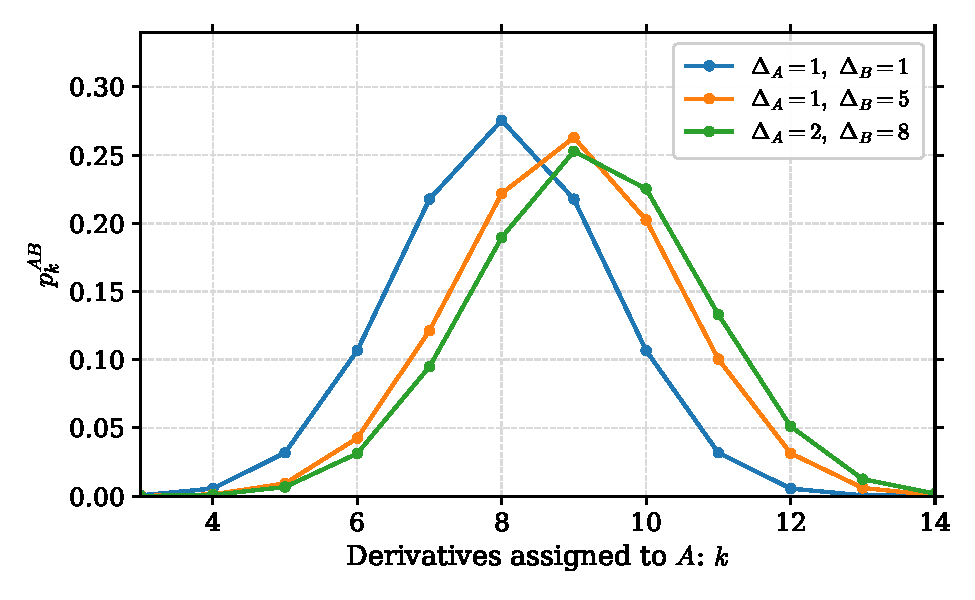
\includegraphics[width=.78\textwidth]{content/FreeElectronQuantumOptics/figures/geometry-highspin/generated/mixed_scalar_modes.pdf}
 \caption{固定 $S=16$ 时，不同标度维数组合的精确双体模式分配概率。所有曲线都由 \cref{eq:ghs-r4-mixed-mode-probability} 计算；峰位发生变化来自两种标量的维数不同，而不是某个额外耦合常数。}
 \label{fig:ghs-r4-mixed-scalar-modes}
\end{figure}

对于固定 $\Delta_A,\Delta_B$ 且 $S\to\infty$，主导项来自 $k=S/2+O(\sqrt S)$。Stirling 展开说明两个 $\binom Sk$ 因子决定指数部分，而 Pochhammer 比值只贡献随 $k/S$ 缓变的代数因子，于是中心区的概率逼近
\begin{equation}\label{eq:ghs-r4-mixed-mode-clt}
 p_k^{AB}=\sqrt{\frac{4}{\pi S}}\,
 \exp\left[-\frac{4(k-S/2)^2}{S}\right]
 \bigl[1+O(S^{-1/2})\bigr],
\end{equation}
其中误差限于 $|k-S/2|\le C\sqrt S$、固定 $C$ 的中心区，且 $\Delta_A,\Delta_B$ 随 $S$ 固定。于是 $\operatorname{Var}(k)=S/8+O(1)$；若标度维数自身随 $S$ 增长，则必须重新分析鞍点，不能直接使用上述高斯。对 $\Delta_A=\Delta_B=1$，\cref{eq:ghs-r4-mixed-mode-probability} 恢复先前得到的 $\binom Sk^2/\binom{2S}S$。


用 Gamma 函数将 \cref{eq:ghs-r4-mixed-mode-probability} 中依赖 $k$ 的部分重新整理为
\begin{equation*}
 p_k^{AB}\propto\binom Sk^2
 \frac{\Gamma(k+1)}{\Gamma(k+\Delta_A)}
 \frac{\Gamma(S-k+1)}{\Gamma(S-k+\Delta_B)}.
\end{equation*}
在 $k$ 和 $S-k$ 同时增大的区域，Gamma 比值的 Stirling 公式给出
\begin{equation*}
 \frac{\Gamma(k+1)}{\Gamma(k+\Delta_A)}
 =k^{1-\Delta_A}[1+O(k^{-1})],
\end{equation*}
另一因子相同，只需替换 $k\mapsto S-k$ 与 $\Delta_A\mapsto\Delta_B$。现在写 $k=S/2+x$，固定 $\Delta_A,\Delta_B$，并让 $|x|\le C\sqrt S$。二项式系数的中心区展开为
\begin{equation*}
 2\log\binom S{S/2+x}
 =2S\log2-\log(\pi S/2)-\frac{4x^2}{S}
 +O(S^{-1}),
\end{equation*}
其中余项对固定 $C$ 一致有界。对剩下的代数因子展开对数：
\begin{align*}
 &(1-\Delta_A)\log(S/2+x)
 +(1-\Delta_B)\log(S/2-x)\\
 &\quad=\text{与 $x$ 无关的项}
 +\frac{2(\Delta_B-\Delta_A)x}{S}+O(S^{-1}).
\end{align*}
所以概率的中心区对数可写为
\begin{equation*}
 \log p_k^{AB}=\text{归一化常数}
 -\frac4S\left(x-\frac{\Delta_B-\Delta_A}{4}\right)^2
 +O(S^{-1}).
\end{equation*}
用 \(\sum_k\exp(-4(k-S/2)^2/S)\sim\sqrt{\pi S}/2\) 归一化，得到 \cref{eq:ghs-r4-mixed-mode-clt}。连续鞍点相对 $S/2$ 的位移是 $(\Delta_B-\Delta_A)/4+O(S^{-1})$；实际离散分布的众数须再取最接近鞍点的整数，不能把它们混为一谈。二次项的曲率给出领先方差 $S/8$。若要得到 $O(1)$ 的方差修正，则应保留 Stirling 展开中下一阶的四次项及归一化修正。


这一计算揭示了自由高自旋态中比对径峰更普适的对象：在同一共形表示的最低扭度层上，两个标量如何分享总径向能量。构成场的标度维数可以任意变化，中心区的 $\sqrt S$ 宽度却保持不变；这是由共形初级约束和广义自由因子化共同产生的结果，而不是某个特定四维球谐积分的巧合。


\subsection{无迹极化与自旋关联的张量恢复}

零极化多项式隐藏了迹项，二点函数和守恒条件却会重新调用这些项。为使张量缩并自足，固定恢复规则。

\begin{definition}[调和投影与零锥导数]
令 $F_S(z)$ 为 $d$ 维辅助向量 $z$ 的齐次 $S$ 次多项式。其对称无迹投影为
\begin{equation}\label{eq:ghs-r4-stf-projector}
 \Pi_SF_S=\sum_{k=0}^{\lfloor S/2\rfloor}
 \frac{(-1)^k\Gamma(S+d/2-k-1)}{4^kk!\Gamma(S+d/2-1)}
 (z^2)^k(\partial_z^2)^kF_S.
\end{equation}
$S=0$ 单独定义 $\Pi_0=1$。令 $\nu=d/2-1$，作用于零锥等价类的 Thomas 导数为
\[
 \mathcal D_{z,\mu}=(\nu+z\cdot\partial_z)\partial_{z,\mu}
 -\tfrac12z_\mu\partial_z^2.
\]
它将 $z^2$ 倍数映为 $z^2$ 倍数，因此 $\partial_x^\mu\mathcal D_{z,\mu}J_S$ 与多项式代表无关。完整投影递推与任意秩证明可参照《群论》的对称无迹张量部分。
\end{definition}
\begin{proof}
对齐次 $m$ 次多项式 $G_m$，
\[
 \partial_z^2[(z^2)^kG_m]=(z^2)^k\partial_z^2G_m
 +4k(m+k+d/2-1)(z^2)^{k-1}G_m.
\]
代入 $m=S-2k$，相邻迹阶系数满足
$a_{k+1}=-a_k/[4(k+1)(S-k+d/2-2)]$，$a_0=1$，得到 Gamma 形式；最高阶以后重复 Laplace 运算为零。

对 Thomas 导数展开 $\mathcal D_{z,\mu}(z^2G_m)$。不含 $z^2$ 的项为
$[2(\nu+m+1)-(d+2m)]z_\mu G_m=0$，所以改变零锥多项式代表不会改变散度条件。
\end{proof}


对一般的对称无迹初级算符 $J_{\Delta,S}$，仅由平移、旋转和尺度不变性还不能固定它的二点函数；必须再处理反演。令
\begin{equation}\label{eq:ghs-r4-inversion-matrix}
 I_{\mu\nu}(x)=\delta_{\mu\nu}-2\frac{x_\mu x_\nu}{x^2},\qquad
 I_{\mu\rho}(x)I_{\rho\nu}(x)=\delta_{\mu\nu}.
\end{equation}
它是反演坐标映射在正交标架中的反射矩阵。把每个自旋指标都用 $I_{\mu\nu}$ 连接两个端点，然后取无迹部分，得到一般二点函数
\begin{equation}\label{eq:ghs-r4-general-stt-two-point}
 \langle J_{\Delta,S}(x_1,z_1)J_{\Delta,S}(x_2,z_2)\rangle
 =\frac{C_J}{(x_{12}^2)^\Delta}
 \Bigl[z_1^\mu I_{\mu\nu}(x_{12})z_2^\nu\Bigr]^S,
 \quad z_1^2=z_2^2=0.
\end{equation}
$C_J$ 只取决于对 $J$ 的归一化。不同 $\Delta,S$ 或不同不可约内部对称性表示之间，标准的共形二点函数为零。若以后需要作迹、散度或张量指标缩并，必须以 \cref{eq:ghs-r4-stf-projector} 对上述右侧恢复其无迹多项式延拓。


复合共形变换对 $x$ 的作用含有分式映射，直接用它变换多个高自旋指标相当繁琐。对任意整数 $d>2$，可引入具有签名 $(d+1,1)$ 的辅助空间 $\RR^{d+1,1}$，采用坐标 $P^A=(P^+,P^-,P^\mu)$，内积
\begin{equation}\label{eq:ghs-r4-embedding-inner-product}
 P\cdot Q=-\frac12(P^+Q^-+P^-Q^+)+\delta_{\mu\nu}P^\mu Q^\nu.
\end{equation}
将欧氏点 $x$ 送入射影零锥
\begin{equation}\label{eq:ghs-r4-embedding-section}
 P(x)=(1,x^2,x^\mu),\qquad P(x)^2=0,\qquad
 -2P(x)\cdot P(y)=(x-y)^2.
\end{equation}
因此对 $P$ 的一个线性 $SO(d+1,1)$ 变换，在选定 $P^+=1$ 截面以后，就是原来对 $x$ 的非线性共形变换。这项几何化并未引入额外的物理时空维度；射影等价 $P\sim\lambda P$ 正好去掉辅助坐标多出来的尺度。

自旋极化向量同时提升为
\begin{equation}\label{eq:ghs-r4-embedding-polarization}
 Z(x,z)=(0,2x\cdot z,z^\mu),\qquad
 Z\cdot P=0,\qquad Z^2=z^2=0.
\end{equation}
嵌入空间的张量多项式 $\mathcal J(P,Z)$ 满足 $\mathcal J(\lambda P,Z)=\lambda^{-\Delta}\mathcal J(P,Z)$、$\mathcal J(P,\alpha Z)=\alpha^S\mathcal J(P,Z)$，并具有规范等价 $Z\sim Z+\beta P$。前两个齐次条件分别记录标度维数与自旋，最后一个条件去掉非物理的径向指标。它们不是三项任意的写作约定，而是原有张量变换律在射影零锥上的表述 \cite{ghs-costa}。


构造三点函数时，距离平方来自 $P_{ij}=-2P_i\cdot P_j$。对于第三个点的极化，具有规范不变性的唯一线性结构可取
\begin{equation}\label{eq:ghs-r4-embedding-V}
 V_{3,12}=\frac12\left(\frac{Z_3\cdot P_1}{P_3\cdot P_1}
 -\frac{Z_3\cdot P_2}{P_3\cdot P_2}\right)
 =z\cdot\left(\frac{x_{31}}{x_{31}^2}-\frac{x_{32}}{x_{32}^2}\right).
\end{equation}
在 $Z_3\mapsto Z_3+\beta P_3$ 下，两项各加上相同的 $\beta$，所以它们的差不变。设 $\tau=\Delta-S$ 为交换初级算符的扭度，则一般的非零三点函数为
\begin{align}\label{eq:ghs-r4-general-ssj-three-point}
 &\langle A(x_1)B(x_2)J_{\Delta,S}(x_3,z)\rangle\\
 &\quad=\frac{\lambda_{ABJ}\,V_{3,12}^S}
 {(x_{12}^2)^{(\Delta_A+\Delta_B-\tau)/2}
 (x_{23}^2)^{(\Delta_B+\tau-\Delta_A)/2}
 (x_{31}^2)^{(\Delta_A+\tau-\Delta_B)/2}}.\notag
\end{align}
这个结果不要求 $A,B$ 或 $J$ 是广义自由算符。其三个距离指数同时满足各端点所需的标度与反演协变性。将 $J=[AB]_S$、$x_3=0$、$\tau=\Delta_A+\Delta_B$ 代入，就精确恢复 \cref{eq:ghs-r4-general-mixed-threepoint} 的位置依赖；在这个特例中才可以用 Wick 定理进一步算出 $\lambda_{ABJ}$。

两个带自旋算符之间还可以形成
\begin{equation}\label{eq:ghs-r4-embedding-H}
 H_{ij}=(-2P_i\cdot P_j)(Z_i\cdot Z_j)
 +2(Z_i\cdot P_j)(Z_j\cdot P_i).
\end{equation}
在物理截面上 $H_{ij}=x_{ij}^2\,z_i\cdot I(x_{ij})\cdot z_j$。由 $V_i$ 与 $H_{ij}$ 组成的非负整数次单项式，再结合每个点极化向量的次数要求，就形成任意对称无迹外自旋、宇称偶三点张量结构的有限维基底。若在三维使用 Levi--Civita 张量，还会出现宇称奇结构；低维 Schouten 恒等式也会使部分张量结构不独立。因而 \cref{eq:ghs-r4-general-ssj-three-point} 的唯一性专指两个标量和一个对称无迹自旋算符的情形，不能无条件推广为三个任意自旋算符只允许一个系数。


一个对称无迹初级表示的二次 Casimir 本征值已经由 \cref{eq:ghs-casimir-eigenvalue} 得到：
\begin{equation}\label{eq:ghs-r4-casimir-shadow-symmetry}
 C_{\Delta,S}=\Delta(\Delta-d)+S(S+d-2)
 =C_{d-\Delta,S}.
\end{equation}
因此，只指定自旋和这个本征值，并不能在两支形式解 $\Delta$ 与 $d-\Delta$ 之间作选择。后者对应所谓的影子维数。物理径向块必须再规定 $r\to0$ 的初级态起始行为 $r^\Delta$，以及相应的反射正性和后裔结构；影子支一般不能当成同一个算符乘积展开中的另一个物理初级态。$\Delta=d/2$ 附近两支相遇时，某些微分方程的第二个局部解会出现对数，需要按极限和边界条件分别处理。这些事实解释了为什么共形块是有明确边界条件的 Casimir 解，而不仅是一条本征值方程。


共形生成元决定初级态及其后裔的结构。将这些态重新放回局域关联函数，就能由三点函数计算算符乘积中的展开系数。


\section{三点函数与 OPE}
\label{sec:ghs-three-point-ope}


一个算符在球面上制备什么态，是径向量子化的运动学问题；两个算符靠近时会激发哪些态，则决定了量子场论的相互作用数据。在自由标量场中，这两个问题通过同一组 Wick 收缩相连。前面求出的 $(z_1-z_2)^S$ 其实已经是一个自旋 $S$ 三点函数在等半径球面上的截面。这一部分将恢复完整的空间依赖，并说明它怎样进入算符乘积展开。


记 $G(x)=C_d/|x|^{2\delta}$，并将自由标量重新标准化为 $\chi=\varphi/\sqrt{C_d}$，使 $\langle\chi(x)\chi(0)\rangle=|x|^{-2\delta}$。自旋 $S$ 的初级算符 $\mathcal O_S$ 仍采用 \cref{eq:ghs-bilinear-general,eq:ghs-primary-coefficients} 的约定。把它除以 \cref{eq:ghs-operator-norm} 的径向范数，定义归一最高权算符
\begin{equation}\label{eq:ghs-normalized-highest-current}
 \mathscr J_S(x;\vb\varepsilon)=\frac{\mathcal O_S(x;\vb\varepsilon)}{\sqrt{\mathcal N_S}},
 \qquad \mathcal N_S=2^{2S+1}C_d^2S!(2\delta+S-1)_S.
\end{equation}
这里的“归一”特指选定复零极化最高权态的径向范数为一。它与某些文献把全部张量指标收缩得到的 $C_J=1$ 约定未必相同；比较文献中的 OPE 系数时必须同时转换极化向量归一化。

取 $x_3=0$，令
\begin{equation}\label{eq:ghs-threepoint-polarization-invariant}
 V_3(x_1,x_2;\vb\varepsilon)
 =\vb\varepsilon\cdot\left(\frac{x_1}{|x_1|^2}-\frac{x_2}{|x_2|^2}\right).
\end{equation}
从自由传播子求导并利用前文初级递推式，直接得到偶数自旋的三点函数
\begin{equation}\label{eq:ghs-scalar-scalar-spin-3pt}
 \langle\chi(x_1)\chi(x_2)\mathscr J_S(0;\vb\varepsilon)\rangle
 =g_S\frac{V_3(x_1,x_2;\vb\varepsilon)^S}
 {|x_1|^{2\delta}|x_2|^{2\delta}},
 \qquad
 g_S=\frac{\sqrt2(\delta)_S}{\sqrt{S!(2\delta+S-1)_S}}.
\end{equation}
位置因子是共形对称允许的标量—标量—对称无迹张量三点函数结构。动力学只保留在一个数 $g_S$ 中。在一般 CFT 中，维数可以不等于 $2\delta+S$，分母幂次须相应改变，且 $g_S$ 不再由 Wick 定理给出。


\begin{proof}
令 $D_3=\vb\varepsilon\cdot\partial_{x_3}$。对两条自由传播线分别求导，零极化条件给出
\begin{equation*}
D_3^kG(x_1-x_3)|_{x_3=0}
=2^k C_d(\delta)_k
\frac{(\vb\varepsilon\cdot x_1)^k}{|x_1|^{2\delta+2k}}.
\end{equation*}
正规序使第三点的两个场只与外场配对。把所有 $k$ 的贡献加总并用 $c_k(\delta)_k(\delta)_{S-k}=(-1)^k\binom Sk(\delta)_S$，得到
\begin{align*}
&\langle\varphi(x_1)\varphi(x_2)\mathcal O_S(0;\vb\varepsilon)\rangle\\
&\quad=2^{S+1}C_d^2(\delta)_S
|x_1|^{-2\delta}|x_2|^{-2\delta}
\sum_{k=0}^S(-1)^k\binom Sk
\left(\frac{\vb\varepsilon\cdot x_1}{|x_1|^2}\right)^k
\left(\frac{\vb\varepsilon\cdot x_2}{|x_2|^2}\right)^{S-k}\\
&\quad=2^{S+1}C_d^2(\delta)_S
|x_1|^{-2\delta}|x_2|^{-2\delta}
\left(\frac{\vb\varepsilon\cdot x_2}{|x_2|^2}
-\frac{\vb\varepsilon\cdot x_1}{|x_1|^2}\right)^S.
\end{align*}
偶数 $S$ 去掉了最后括号里的整体负号；除以两个 $\sqrt{C_d}$ 与一个 $\sqrt{\mathcal N_S}$，系数变为
\begin{equation*}
\frac{2^{S+1}C_d(\delta)_S}{\sqrt{2^{2S+1}C_d^2S!(2\delta+S-1)_S}}
=\frac{\sqrt2(\delta)_S}{\sqrt{S!(2\delta+S-1)_S}}.
\end{equation*}
\end{proof}

在自旋零的情形，$\mathscr J_0=:\!\chi^2\!:/\sqrt2$，所以 $g_0=\sqrt2$，与直接计算 $\langle\chi\chi:\!\chi^2\!:\rangle=2G_\chi G_\chi$ 完全一致。四维时还可得到
\begin{equation}\label{eq:ghs-threepoint-four-d}
 g_S^2=\frac{2(S!)^2}{(2S)!}
 =\frac2{\binom{2S}{S}},\qquad d=4,\quad S\in2\NN_0.
\end{equation}
这个系数随自旋快速变小，并不意味着相应的高自旋流“消失”：张量结构 $V_3^S$ 与归一约定也随自旋变化，不能只比较裸系数。


\subsection{局域算符乘积与后裔系数}

设一般 CFT 中两个初级算符 $A(x),B(0)$ 相距很近。取一个球面包围二者而不包围其他插入，球内路径积分制备的态可依径向 哈密顿量 的一组完备本征态展开。这些本征态按共形初级态及其 $P_\mu$ 后裔分组，产生局域算符乘积展开：
\begin{equation}\label{eq:ghs-ope-general}
 A(x)B(0)=\sum_{\mathcal O}\mathcal C_{AB\mathcal O}(x,\partial)
 \mathcal O(0).
\end{equation}
这里 $\mathcal C$ 是确定后裔系数的微分算符值函数；求和不仅包含初级算符，还隐含其所有后裔。在两点可被同一个球面与其余插入严格分隔的欧氏相关函数中，此展开可以通过径向 Hilbert 空间的谱表示理解其收敛性，参见 \cite{ghs-rychkov,ghs-simmons}。若只截留初级算符而抛掉后裔，通常得不到共形协变的四点函数。

在自由标量场中，乘积可以先用 Wick 定理逐项精确拆开：
\begin{equation}\label{eq:ghs-free-field-ope-start}
 \chi(x)\chi(0)=\frac{\mathds1}{|x|^{2\delta}}+\, :\!\chi(x)\chi(0)\!:.
\end{equation}
第二项在 $x=0$ 附近 Taylor 展开，第一项为 $:\!\chi^2\!:=\sqrt2\,\mathscr J_0$。但剩余的导数项既包含新的高自旋初级流，也包含前面已经出现的标量和低自旋流的平移后裔。因此不能把 Taylor 展开中的每一个导数单项式都当成独立初级算符。


\cref{eq:ghs-spin-unitarity-bound-extended} 表明 $\Delta_S=S+d-2$ 对 $S\ge1$ 正好意味着散度后裔被截去。前面所构造的每个偶数自旋 $S\ge2$ 双线性流都满足这一条件。于是 $\chi\times\chi$ 中不仅出现单位算符和标量 $:\!\chi^2\!:$，还包含无穷多个高自旋短表示。它们不是由一个有限个基本场的额外粒子谱手工添进去的，而是两个自由场组成的复合算符。

反过来，若将基本标量换成标度维数 $\Delta_\chi>\delta$ 的一般初级算符，两个算符乘积中典型的双算符初级态具有近似或精确的自由组合维数
\begin{equation}\label{eq:ghs-doubletwist-kinematic-dimension}
 \Delta_{n,S}^{(0)}=2\Delta_\chi+2n+S,
 \qquad n=0,1,\ldots .
\end{equation}
这里 $n$ 计数相对导数的额外两阶，$S$ 是总对称无迹自旋。对于真正的广义自由场，这些是独立算符；对于饱和标量幺正界的局域自由场，运动方程会使部分本来形式独立的高阶后裔成为零范数，谱必须作相应约化。在相互作用理论中，双算符态通常还获得反常维数。


径向量子化的初级态能量 $\Delta_{\mathcal O}$ 和角动量表示说明“有哪些态”；三点函数系数 $\lambda_{AB\mathcal O}$ 则说明两次局域插入怎样激发这些态。给定局域共形代数和一套统一的算符归一化，完整的标度维数与三点函数系数构成局域共形数据。四点及更高相关函数应由它们的算符乘积展开重建，但同一四点函数可以按不同配对次序展开，必须得到一致结果。这一条件将不再允许谱和系数任意选择。


径向量子化告诉我们：把两个插入点圈进同一个球面之后，球内的态必须能在一组共形初级态及其后裔上展开。不过，知道哪些初级态出现还不够。若把一对局域算符移动一点距离，为什么初级态的一阶、二阶后裔会以特定比例被激发？这些比例必须由共形代数决定，否则同一乘积的三点函数就不可能与全局共形协变性相容。


考虑三个标量初级算符 $A,B,\mathcal O$，其维数分别为 $\Delta_A,\Delta_B,\Delta>0$；将 $\mathcal O$ 的两点函数归一为
\begin{equation}\label{eq:ghs-ope-scalar-normalization}
 \langle\mathcal O(x)\mathcal O(0)\rangle=(x^2)^{-\Delta}.
\end{equation}
暂取三种算符互不简并，也不包含相同量子数的混合。共形对称把三点函数固定为
\begin{equation}\label{eq:ghs-ope-three-scalar}
 \langle A(x)B(0)\mathcal O(y)\rangle
 =\frac{\lambda_{AB\mathcal O}}
 {(x^2)^{(\Delta_A+\Delta_B-\Delta)/2}
 (y^2)^{(\Delta_B+\Delta-\Delta_A)/2}
 ((y-x)^2)^{(\Delta_A+\Delta-\Delta_B)/2}}.
\end{equation}
这里 $x^2=|x|^2$，并假定 $|x|<|y|$，使围住 $x,0$ 的球面不包含第三个插入点。令
\begin{equation}\label{eq:ghs-ope-alpha-beta}
 \alpha=\frac{\Delta+\Delta_A-\Delta_B}{2},\qquad
 \beta=\frac{\Delta+\Delta_B-\Delta_A}{2},\qquad
 \alpha+\beta=\Delta.
\end{equation}
我们把该初级表示在乘积中的贡献写成以下局域展开：
\begin{align}\label{eq:ghs-ope-scalar-level-two}
 A(x)B(0)\big|_{\mathcal O}
 =&\;\lambda_{AB\mathcal O}(x^2)^{(\Delta-\Delta_A-\Delta_B)/2}
 \bigl[\mathcal O(0)+a\,x^\mu\partial_\mu\mathcal O(0)
 \\&\qquad+b\,x^2\partial^2\mathcal O(0)
 +c\,x^\mu x^\nu\partial_\mu\partial_\nu\mathcal O(0)
 +O(|x|^3)\bigr].\notag
\end{align}
$a,b,c$ 是无量纲数。二阶存在两个独立的旋转标量结构：一个由迹 $\partial^2\mathcal O$ 构成，另一个由沿 $x$ 方向的二次导数构成。把它们混成一个“二阶项”，就无法看见零范数后裔对应的极点。


将 \cref{eq:ghs-ope-three-scalar} 除以共同的 $\lambda_{AB\mathcal O}(x^2)^{(\Delta-\Delta_A-\Delta_B)/2}(y^2)^{-\Delta}$，左侧剩下
\begin{equation}\label{eq:ghs-ope-kinematic-ratio}
 F(x,y)=\left(1-2\frac{x\cdot y}{y^2}+\frac{x^2}{y^2}\right)^{-\alpha}.
\end{equation}
取 $t=(x\cdot y)/y^2$ 与 $u=x^2/y^2$，按 $|x|/|y|$ 的次数展开：
\begin{equation}\label{eq:ghs-ope-ratio-expansion}
 F(x,y)=1+2\alpha t-\alpha u+2\alpha(\alpha+1)t^2
 +O\bigl((|x|/|y|)^3\bigr).
\end{equation}
这一行来自 $(1+q)^{-\alpha}=1-\alpha q+\alpha(\alpha+1)q^2/2+\cdots$；其中 $u$ 已是二阶，故不能把 $u^2$ 保留在当前阶数中。

右侧的后裔算符与 $\mathcal O(y)$ 做两点函数时，对 $\mathcal O(0)$ 的求导等于对 $y$ 求导的负号。这一点直接决定了一阶系数的符号。我们有
\begin{align*}
 x^\mu\partial_{0\mu}(y^2)^{-\Delta}
 &=2\Delta t(y^2)^{-\Delta},\\
 x^\mu x^\nu\partial_{0\mu}\partial_{0\nu}(y^2)^{-\Delta}
 &=\bigl[-2\Delta u+4\Delta(\Delta+1)t^2\bigr](y^2)^{-\Delta},\\
 x^2\partial_0^2(y^2)^{-\Delta}
 &=2\Delta(2\Delta+2-d)u(y^2)^{-\Delta}.
\end{align*}
按 $t,t^2,u$ 三种独立的角结构分别比较系数，得到完整的二阶结果：
\begin{equation}\label{eq:ghs-ope-descendant-coefficients}
 a=\frac{\alpha}{\Delta},\qquad
 c=\frac{\alpha(\alpha+1)}{2\Delta(\Delta+1)},\qquad
 b=-\frac{\alpha\beta}{2\Delta(\Delta+1)(2\Delta+2-d)}.
\end{equation}
因此，对于一般非零范数的标量初级表示，\cref{eq:ghs-ope-scalar-level-two} 的前两级后裔没有自由参数：只要已知三个标度维数和一个初级 OPE 系数，整个后裔比例就确定了。


\begin{proof}
一阶和二阶无迹方向的系数由
\begin{align*}
2\Delta a&=2\alpha,\\
4\Delta(\Delta+1)c&=2\alpha(\alpha+1)
\end{align*}
给出。二阶迹结构的系数必须满足
\begin{align*}
2\Delta(2\Delta+2-d)b-2\Delta c&=-\alpha,\\
2\Delta(2\Delta+2-d)b
&=-\alpha+\frac{\alpha(\alpha+1)}{\Delta+1}\\
&=\frac{\alpha(\alpha-\Delta)}{\Delta+1}
=-\frac{\alpha\beta}{\Delta+1}.
\end{align*}
最后使用 $\beta=\Delta-\alpha$，即得 \cref{eq:ghs-ope-descendant-coefficients}。这些计算只要求 $x$ 与 $y$ 不重合，并在 $|x|<|y|$ 的欧氏径向域中进行；如果初级表示含零范数态，下式的反矩阵步骤必须先取商空间。
\end{proof}

二级迹后裔的范数已由 \cref{eq:ghs-scalar-unitarity-bound} 的推导确定：
\begin{equation}\label{eq:ghs-ope-trace-norm-repeat}
 \|P^2|\mathcal O\rangle\|^2
 =8d\Delta\left(\Delta-\frac{d-2}{2}\right)
 \|\mathcal O\|^2.
\end{equation}
另一方面，$b$ 的分母中有 $2\Delta+2-d=2(\Delta-(d-2)/2)$。两者在同一点消失。这不是一个偶然的代数分母：构造 OPE 后裔系数需要反演该级的 Gram 矩阵；如果一个后裔成为零范数态，该矩阵不再可逆。

当 $\Delta=(d-2)/2$，若 $\alpha\beta\ne0$，形式上的 $b$ 发散。对连续、单位的共形场论，饱和标量幺正性界的算符满足自由运动方程；只允许与其零模一致的相关函数耦合。对所考虑的单个非零三点函数，这要求 $\alpha\beta=0$，以便零范数子表示不产生矛盾。不能将一个一般 $\alpha\beta\ne0$ 的形式级数在分母处直接代入 $\Delta=(d-2)/2$。

再看两个相同外场 $A=B$。这时 $\alpha=\beta=\Delta/2$，并且
\begin{equation}\label{eq:ghs-identical-scalar-descendants}
 a=\frac12,\quad
 c=\frac{\Delta+2}{8(\Delta+1)},\quad
 b=-\frac{\Delta}{8(\Delta+1)(2\Delta+2-d)}.
\end{equation}
其中 $a=1/2$ 有直观解释：交换两端相同的算符，同时将 OPE 的展开原点由一个端点平移到另一个端点，一阶平移应由两端对称分担。二阶系数却不是仅凭这种交换对称就能猜出的；它同时包含迹通道的共形几何。


从 Hilbert 空间看，上述计算还有一个更普适的形式。固定由某个初级态 $|\mathcal O\rangle$ 产生的后裔表示，在每一级选出一组线性独立态 $|a\rangle$，其 Gram 矩阵为 $G_{ab}=\langle a|b\rangle$。该级表示的正交投影是
\begin{equation}\label{eq:ghs-ope-gram-projector}
 \Pi_{\mathcal O,n}=\sum_{a,b\in\mathcal H_{\mathcal O,n}}
 |a\rangle\,(G^{-1})^{ab}\,\langle b|.
\end{equation}
它满足 $\Pi^2=\Pi$，其原因是中间两个 Gram 矩阵相乘后给出单位矩阵。把投影插入包围两点的球面态展开，便得到 OPE 系数。改变后裔基底不会改变 $\Pi$，所以实际相关函数不依赖我们选的是迹/无迹分解还是其他等价基底。

若某一级出现零范数后裔，首先在物理 Hilbert 空间中将其模掉，再反演剩余非退化 Gram 矩阵。初级表示缩短时，共形块也随之发生相应的极点与残数结构；这正是以后用 Casimir 方程和谱极点研究多重态重组的数学基础。参见 \cite{ghs-rychkov,ghs-simmons,ghs-rychkov-tan}。

径向 Hilbert 空间的后裔谱由共形代数产生，算符乘积展开则记录不同初级如何耦合。四点函数使这些数据彼此约束：不同的算符配对次序必须得到同一个相关函数。


算符乘积展开把一个相关函数分成各个初级表示及其后裔。四个算符却可以按不止一种次序配对，因此相同的四点函数为这些表示数据施加了额外的相容条件。


只有两点函数和三点函数时，共形对称给出的限制仍很宽：不同初级算符的维数与三点函数常数可以分别输入。四点函数第一次让这些数据必须相互兼容，因为四个算符可以先把前两个配对，也可以先把中间两个配对。所谓共形自举，就是把这种不依赖配对顺序的恒等关系与幺正性、谱信息结合起来。


取四个互不重合的欧氏点 $x_i\in\RR^d$，记 $x_{ij}=x_i-x_j$，$x_{ij}^2=|x_i-x_j|^2$。四个相同标量初级算符 $\mathcal X$ 的标度维数取 $\Delta_\mathcal X$，其二点函数标准化为 $\langle\mathcal X(x)\mathcal X(0)\rangle=(x^2)^{-\Delta_\mathcal X}$。共形变换只能将四点坐标约化为两个独立交比
\begin{equation}\label{eq:ghs-cross-ratios}
 U=\frac{x_{12}^2x_{34}^2}{x_{13}^2x_{24}^2},
 \qquad V=\frac{x_{14}^2x_{23}^2}{x_{13}^2x_{24}^2}.
\end{equation}
于是其相关函数的一般形式是
\begin{equation}\label{eq:ghs-fourpoint-reduced}
 \langle\mathcal X_1\mathcal X_2\mathcal X_3\mathcal X_4\rangle
 =\frac{\mathcal G(U,V)}{(x_{12}^2x_{34}^2)^{\Delta_\mathcal X}}.
\end{equation}
函数 $\mathcal G$ 无法单靠共形协变性确定，因为它包含真实的 OPE 动力学。交换第 $2$、$4$ 个相同场时，$(U,V)$ 变成 $(V,U)$，同时外面的距离因子发生变化。将同一个四点函数写成两种方式，得到交叉对称方程
\begin{equation}\label{eq:ghs-crossing-scalar}
 V^{\Delta_\mathcal X}\mathcal G(U,V)
 =U^{\Delta_\mathcal X}\mathcal G(V,U).
\end{equation}
它是严格的相关函数恒等式，不是大自旋近似。


对前面标准化的自由标量 $\chi$，三个 Wick 配对穷尽了四点函数：
\begin{align}\label{eq:ghs-free-scalar-fourpoint}
 \langle\chi_1\chi_2\chi_3\chi_4\rangle
 &=\frac1{(x_{12}^2x_{34}^2)^\delta}
 +\frac1{(x_{13}^2x_{24}^2)^\delta}
 +\frac1{(x_{14}^2x_{23}^2)^\delta},\\
 \mathcal G_\chi(U,V)&=1+U^\delta+(U/V)^\delta.\notag
\end{align}
交换 $(U,V)$ 后，
\begin{align*}
 (U/V)^\delta\mathcal G_\chi(V,U)
 &=(U/V)^\delta[1+V^\delta+(V/U)^\delta]\\
 &=(U/V)^\delta+U^\delta+1
 =\mathcal G_\chi(U,V),
\end{align*}
这正是 \cref{eq:ghs-crossing-scalar}。自由场虽然容易计算，却已包含自举中最重要的一点：同一四点函数的三个配对次序彼此相容。

四维共形场论常把两个交比表示为 $U=z\bar z$、$V=(1-z)(1-\bar z)$。在欧氏构型中 $\bar z$ 是 $z$ 的复共轭；将 $z,\bar z$ 作为独立实变量去取光锥极限，则属于分析延拓后的洛伦兹运动学，不能把两种取极限的方式混为一谈。


仅有三个 Wick 配对还不容易看见复合算符之间的连接结构。考虑标准化的双线性标量
\begin{equation}\label{eq:ghs-normalized-phi2}
 \mathcal B(x)=\frac1{\sqrt2}:\!\chi(x)^2\!:,
 \qquad\Delta_\mathcal B=2\delta.
\end{equation}
正规序规定同一点内部不自收缩。四个 $\mathcal B$ 各带两个标量腿，所以完整的 Wick 图既有不连通的双配对，也有四点连成一个圈的三种方式。结果是
\begin{align}\label{eq:ghs-bilinear-fourpoint}
 \mathcal G_\mathcal B(U,V)
 &=1+U^{2\delta}+(U/V)^{2\delta}\\
 &\quad+4\bigl[U^\delta+(U/V)^\delta+(U^2/V)^\delta\bigr].\notag
\end{align}
相比 \cref{eq:ghs-free-scalar-fourpoint}，新增项恰恰记录四个复合算符之间的连接相关。这个例子并非相互作用理论：尽管 $\mathcal B$ 的相关函数有连接图，基本场仍然服从高斯 Wick 定理。


自由场四点函数可将全部 Wick 配对按连通结构分类。
记 $G_{ij}=\langle\chi_i\chi_j\rangle=(x_{ij}^2)^{-\delta}$。四个 $:\!\chi^2\!:$ 的 Wick 收缩只允许连接不同顶点。若顶点 $1,2$ 之间两条线、顶点 $3,4$ 之间两条线，则收缩数为 $(2!)(2!)=4$；乘上每个算符的 $1/\sqrt2$ 后，整张图的因子为 $1$，给出 $G_{12}^2G_{34}^2$。另外两种断开配对完全类似。

\begin{proof}
若四个顶点连成圈，固定例如 $1\to2\to3\to4\to1$，每个顶点的两条腿均可交换，产生 $2^4=16$ 种 Wick 配对；四个标准化因子相乘为 $1/4$，因此系数为 $4$。只有三种不等价的四顶点圈，合并后
\begin{align*}
\langle\mathcal B_1\mathcal B_2\mathcal B_3\mathcal B_4\rangle
&=G_{12}^2G_{34}^2+G_{13}^2G_{24}^2+G_{14}^2G_{23}^2\\
&\quad+4(G_{12}G_{23}G_{34}G_{41}
+G_{12}G_{24}G_{43}G_{31}
+G_{13}G_{32}G_{24}G_{41}).
\end{align*}
以 $(G_{12}G_{34})^2$ 除去共同因子，三个圈分别变成 $(U/V)^\delta$、$U^\delta$、$(U^2/V)^\delta$，即得 \cref{eq:ghs-bilinear-fourpoint}。
\end{proof}

将 $\mathcal X(x_1)\mathcal X(x_2)$ 与 $\mathcal X(x_3)\mathcal X(x_4)$ 各自做 OPE，中间传播的是由某个初级态 $|\mathcal O\rangle$ 及全部后裔张成的不可约表示。把该表示的贡献归为一个函数，记作自旋 $S$、初级维数 $\Delta$ 的共形块 $G_{\Delta,S}(U,V)$。选择一致的二点函数和共形块标准化后，四点函数分解为
\begin{equation}\label{eq:ghs-conformal-block-expansion}
 \mathcal G(U,V)=\sum_{\mathcal O\in\mathcal X\times\mathcal X}
 \lambda_{\mathcal X\mathcal X\mathcal O}^2
 G_{\Delta_\mathcal O,S_\mathcal O}(U,V).
\end{equation}
对于相同的厄密标量外算符，反射正性使合适的实归一化下 $\lambda^2\ge0$。单位算符的共形块就是 $1$。这里的 $\lambda$ 必须与定义 $G_{\Delta,S}$ 时使用的张量归一化一致；前文固定复零极化的 $g_S$ 不应未经变换就直接替代为任一软件包中的 $\lambda$。

径向量子化解释了共形块的结构：如果两对算符分别位于相隔欧氏径向时间 $t>0$ 的球面上，中间每个后裔的传播因子都是 $\ee^{-t(\Delta+n)}$。对角度上的同阶态再按旋转表示分解，得到沿径向变量 $r=\ee^{-t}$ 的收敛幂级数，其角依赖由 Gegenbauer 多项式表达。这种展开可以直接用于数值计算；选择更对称的径向坐标可显著加快收敛，见 \cite{ghs-hogervorst}。


对具有非退化不变双线性型 $\kappa_{AB}$ 的半单 Lie 代数 $\mathfrak g$，选取基 $T_A$，其二次 Casimir 定义为
\begin{equation}\label{eq:ghs-abstract-quadratic-casimir}
 C_2=\kappa^{AB}T_AT_B\in U(\mathfrak g),
\end{equation}
其中 $\kappa^{AB}\kappa_{BC}=\delta^A_C$。不变性意味着对任意 $T_C$，有
\[
 [T_C,C_2]=\kappa^{AB}([T_C,T_A]T_B+T_A[T_C,T_B])=0.
\]
第二个等号不是形式交换：将 $[T_C,T_A]=f_{CA}{}^DT_D$ 代入，并利用
$\kappa([T_C,T_A],T_B)+\kappa(T_A,[T_C,T_B])=0$，可见两项的系数逐项抵消。在不可约表示上，Schur 引理保证中心元按标量作用，但同一标量可能来自不等价的表示。因此仅有 Casimir 本征值并不足以识别交换的全部物理态。

在球面的标量函数空间中，旋转生成元平方满足 $\sum_{a<b}L_{ab}^2=-\Delta_{S^{d-1}}$；在一般齐性空间中，Casimir 与几何 Laplace 算子的关系还受所选度规、稳定子表示以及张量丛联络影响。这正是把抽象表示论的本征值用于某个量子场论之前必须补上的几何信息。


如果逐个枚举一个初级算符的全部后裔，共形块计算很快就会变得繁琐。由于同一个共形表示中的全部态具有相同的 Casimir 本征值，可以反过来把求和问题改造成微分方程。按前面 \cref{eq:ghs-conformal-commutators} 的径向约定，定义二阶共形 Casimir 算符
\begin{equation}\label{eq:ghs-conformal-quadratic-casimir}
 \mathcal C_2
 =D^2-\frac12M_{\mu\nu}M_{\mu\nu}
 -\frac12\left(P_\mu K_\mu+K_\mu P_\mu\right).
\end{equation}
这里重复指标从 $1$ 到 $d$ 求和。$M_{\mu\nu}$ 在对称无迹自旋 $S$ 表示中的二次型本征值为 $-S(S+d-2)$ 的两倍；这正是前文球谐本征方程在表示论中的写法。对初级态 $K_\mu|\mathcal O\rangle=0$，另外
\begin{equation*}
 K_\mu P_\mu|\mathcal O\rangle
 =[K_\mu,P_\mu]|\mathcal O\rangle
 =2dD|\mathcal O\rangle=2d\Delta|\mathcal O\rangle.
\end{equation*}
所以得到可复算的 Casimir 本征值
\begin{equation}\label{eq:ghs-casimir-eigenvalue}
 \mathcal C_2|\mathcal O_{\Delta,S}\rangle
 =C_{\Delta,S}|\mathcal O_{\Delta,S}\rangle,
 \qquad C_{\Delta,S}=\Delta(\Delta-d)+S(S+d-2).
\end{equation}
对于初级旋转表示 $\lambda$ 而不只对称无迹自旋 $S$，同一代数计算给出
\begin{equation}\label{eq:ghs-general-conformal-casimir-eigen}
 C_2(\Delta,\lambda)=\Delta(\Delta-d)+C_2^{SO(d)}(\lambda).
\end{equation}
这里 $C_2^{SO(d)}(\lambda)$ 采用与旋转生成元平方相匹配的正号归一化。式中 $\Delta$ 与 $d-\Delta$ 有相同的二次 Casimir；影子分支与物理算符分支的区分需要 OPE 短距离边界条件，而不能仅靠该本征值。

由于 Casimir 与整个共形代数对易，$P_\mu$ 产生的每个后裔都保持同一 $C_{\Delta,S}$。这正是为什么能够用一个方程一次性刻画整座后裔塔。

对于四个相同标量外算符，采用 \cref{eq:ghs-fourpoint-reduced} 的外部距离因子，在 $z,\bar z$ 变量上定义
\begin{align}\label{eq:ghs-casimir-differential-operator}
 \mathcal D&=\mathcal D_z+\mathcal D_{\bar z}
 +(d-2)\frac{z\bar z}{z-\bar z}
 \bigl[(1-z)\partial_z-(1-\bar z)\partial_{\bar z}\bigr],\\
 \mathcal D_w&=w^2(1-w)\partial_w^2-w^2\partial_w.
 \notag
\end{align}
将共形生成元对前两个插入点的联合作用变换为交比导数，可得到共形块的微分方程
\begin{equation}\label{eq:ghs-casimir-block-equation}
 \mathcal D G_{\Delta,S}(z,\bar z)
 =\frac12 C_{\Delta,S}G_{\Delta,S}(z,\bar z).
\end{equation}
该方程本身有多个局部解。真正的交换共形块由 $x_{12}\to0$ 的 OPE 边界行为选出：在径向参数 $r\to0$ 时，其最低阶为 $r^\Delta$ 乘一个表示自旋 $S$ 的 Gegenbauer 多项式，后续阶数对应各级后裔。因而“Casimir 本征值 + OPE 边界条件”比仅知道本征值更完整。


\begin{proof}
对 $S$ 阶对称无迹张量 $J_{\mu_1\cdots\mu_S}$，收缩一个辅助向量 $n^\mu$ 得到 $Y_S(n)=J_{\mu_1\cdots\mu_S}n^{\mu_1}\cdots n^{\mu_S}$。它是齐次调和多项式，满足 $\partial_n^2Y_S=0$。在球坐标 $n=r\widehat n$ 下，利用
\begin{equation*}
\partial_n^2=r^{-2}\bigl[(r\partial_r)^2
+(d-2)r\partial_r+\Delta_{S^{d-1}}\bigr]
\end{equation*}
得到 $-\Delta_{S^{d-1}}Y_S=S(S+d-2)Y_S$。角向拉普拉斯算符正是旋转生成元平方之和 $-\tfrac12 M_{\mu\nu}M_{\mu\nu}$。另一方面，初级态满足 $K_\mu|\mathcal O\rangle=0$，因此
\begin{align*}
\mathcal C_2|\mathcal O\rangle
&=\left[D^2-\frac12M_{\mu\nu}M_{\mu\nu}
-\frac12K_\mu P_\mu\right]|\mathcal O\rangle\\
&=\bigl[\Delta^2+S(S+d-2)-d\Delta\bigr]|\mathcal O\rangle.
\end{align*}
这就得到 \cref{eq:ghs-casimir-eigenvalue}。将四点函数写成 \cref{eq:ghs-fourpoint-reduced}，再用坐标微分形式作用于外部两个标量后化简交比，可得到 \cref{eq:ghs-casimir-differential-operator}；完整的坐标雅可比计算和边界解可查阅 \cite{ghs-simmons,ghs-hogervorst}。
\end{proof}

令 $U=z\bar z$、$V=(1-z)(1-\bar z)$。光锥分析考虑 $z\to0$ 而 $\bar z$ 保留非平凡值；当 $\bar z\to1$ 时，交叉通道中最低扭度的算符会控制奇异项。这里扭度定义为
\begin{equation}\label{eq:ghs-twist-definition}
 \tau_{\mathcal O}=\Delta_{\mathcal O}-S_{\mathcal O}.
\end{equation}
扭度不是平移后裔数，它衡量的是一个给定自旋表示距离幺正性下界的方式。守恒高自旋流具有 $\tau=d-2$，与自旋大小无关；一般相互作用双算符态的扭度则为 $2\Delta_\mathcal X+2n+\gamma_{n,S}$。

在满足通常的单位性、谱离散性和适当聚集条件的 $d>2$ 维 CFT 中，光锥交叉方程意味着当 $S\to\infty$ 时存在扭度趋近于 $2\Delta_\mathcal X+2n$ 的双扭度算符序列，参见 \cite{ghs-komargodski,ghs-fitzpatrick}。这不是声称每个有限自旋都恰好满足该等式。固定自旋与无限自旋、先取 $z\to0$ 与先取 $\bar z\to1$ 等极限的次序，决定了展开能否控制。

交叉对称提供从自由高自旋算符走向一般相互作用理论的关键途径：自由理论给出精确的整座短表示塔；一般理论虽不能再用 Wick 定理构造所有态，却依旧受无限自旋处的交叉通道奇异性约束。光锥极限将把这种约束写成可以研究反常维数的渐近式。


前文的四点函数已经写成共形块之和。每一个块都包含无限多个后裔，因此它并不是一条简单的初级交换线。径向量子化提供了计算这些无限和的办法：让一对算符先制备态，让另一对算符在较晚的径向时间读取这个态，所有后裔就按已知能量依次传播。角向结构由旋转群决定，径向传播则由标度维数决定。


选取四个插入点 $0,r\vb n,\vb n',\infty$，其中 $0<r<1$，两个方向 $\vb n,\vb n'\in S^{d-1}$，并令 $\eta=\vb n\cdot\vb n'$。无穷远处的初级插入按 $\mathcal X(\infty)=\lim_{R\to\infty}R^{2\Delta_{\mathcal X}}\mathcal X(R\vb e)$ 定义。四点函数的交比在这组位置上成为
\begin{equation}\label{eq:ghs-radial-fourpoint-crossratios}
 U=r^2,\qquad V=1-2r\eta+r^2,
 \qquad z=r\ee^{\ii\theta},\quad \bar z=r\ee^{-\ii\theta},\quad\eta=\cos\theta.
\end{equation}
$z,\bar z$ 在这里互为复共轭，$r$ 是球半径之比；对应的两次算符制备之间的径向时间差为 $t=-\log r>0$。

考虑交换初级算符 $\mathcal O_{\Delta,S}$ 的整个表示，$S$ 是非负整数。按第 $n$ 级后裔 Hilbert 子空间 $\mathcal H_{\Delta,S;n}$ 插入完备关系，并将第 $n$ 级按 $SO(d)$ 的角动量 $j$ 分解，得到形式精确的谱展开
\begin{equation}\label{eq:ghs-radial-block-expansion}
 G_{\Delta,S}(r,\eta)
 =r^{\Delta}\sum_{n=0}^{\infty}r^n
 \sum_{j\in\mathcal J_n}a_{n,j}
 \frac{C_j^{(\nu)}(\eta)}{C_j^{(\nu)}(1)},
 \qquad \nu=\frac{d-2}{2},\quad d>2.
\end{equation}
$C_j^{(\nu)}$ 是 Gegenbauer 多项式。最低级仅有 $j=S$，故通过选择块的整体标准化可以令 $a_{0,S}=1$。更高一级的 $j$ 由给定初级表示与若干平移生成元的旋转表示张量积分解决定。$a_{n,j}$ 还取决于外部算符维数和共形块归一化；它们不是任意可调的动力学耦合。对反射对称的相同标量外态，可把各级系数写成归一投影范数的和，从而建立非负性。这里为了使首项直观地等于 $r^\Delta C_S^{(\nu)}(\eta)/C_S^{(\nu)}(1)$，采用 $a_{0,S}=1$ 的归一化；下文的四维闭式解沿用常见的超几何块约定，它的首项系数改为 $C_S^{(1)}(1)/2^S$。两种定义只相差交换表示整体的常数因子，比较 OPE 系数时必须同时转换。

这正是 \cref{eq:ghs-ope-gram-projector} 的一个应用：先按初级表示投影，再按后裔能量和角动量投影。$n$ 级项比初级项额外多出 $r^n=\ee^{-nt}$；因此两对算符隔开的径向时间越长，截去高能级后裔造成的误差越小。


从径向路径积分制备的态 $|\Psi_\mathrm{in}\rangle$ 与 $|\Psi_\mathrm{out}\rangle$ 出发，在适当消去外部运动学因子后，四点函数是
\begin{equation}\label{eq:ghs-radial-matrix-element}
 \langle\Psi_\mathrm{out}|\ee^{-tD}|\Psi_\mathrm{in}\rangle.
\end{equation}
在正定 Hilbert 空间中插入同一初级表示的正交投影和各能级投影 $\Pi_n$，每一级便带有因子 $\ee^{-t(\Delta+n)}$。设归一化后的第 $n$ 级矩阵元为 $b_n$，则由 Cauchy--Schwarz 不等式
\begin{align*}
 \sum_n|b_n|r^n
 &\le\left(\sum_n\|\Pi_n\Psi_\mathrm{out}\|^2r^n\right)^{1/2}
       \left(\sum_n\|\Pi_n\Psi_\mathrm{in}\|^2r^n\right)^{1/2}
\end{align*}
可知，只要球面插入分离、经过必要的短距离正规化且两侧制备态范数有限，该展开在 $r<1$ 的相关径向区域内绝对收敛。若在某个 $r_0<1$ 已知 $\sum_{n\ge0}|b_n|r_0^n=M(r_0)<\infty$，则对 $0<r<r_0$，截断至 $N$ 级的误差满足
\begin{equation}\label{eq:ghs-radial-tail-bound}
 \left|\sum_{n>N}b_nr^n\right|
 \le M(r_0)\left(\frac r{r_0}\right)^{N+1}.
\end{equation}
这个界不要求各项同号，因而不仅适用于自由理论。这里 $M(r_0)$ 依赖具体外态及所选块，不能被偷换成独立于共形数据的常数；$r\to1$ 时固定的 $r_0$ 界也不再有效。实际数值自举必须依据所用坐标与截断范围单独控制误差。


虽然 \cref{eq:ghs-radial-block-expansion} 适用于一般维度，$d=4$ 的四个相同标量外算符还有一种特殊优势：Casimir 方程可以化成两个单变量方程。定义
\begin{equation}\label{eq:ghs-block-hypergeometric}
 k_\beta(w)=w^{\beta/2}\,{}_2F_1\left(\frac\beta2,\frac\beta2;\beta;w\right),
 \quad k_0(w)\equiv1.
\end{equation}
这里 $w\in(0,1)$ 时取实主支，其他位置通过解析延拓定义。超几何方程保证
\begin{equation}\label{eq:ghs-block-k-ode}
 \bigl[w^2(1-w)\partial_w^2-w^2\partial_w\bigr]k_\beta(w)
 =\frac{\beta(\beta-2)}4k_\beta(w).
\end{equation}
把两个本征函数反对称组合，自动满足交换 $z\leftrightarrow\bar z$ 的几何对称性。按照 \cref{eq:ghs-casimir-block-equation} 的块约定，偶数自旋的四维精确解可写成
\begin{align}\label{eq:ghs-four-dimensional-exact-block}
 G_{\Delta,S}(z,\bar z)
 ={}&\frac{1}{2^S}\frac{z\bar z}{z-\bar z}
 \bigl[k_{\Delta+S}(z)k_{\Delta-S-2}(\bar z)\\
 &\hspace{7em}-k_{\Delta+S}(\bar z)k_{\Delta-S-2}(z)\bigr],
 \qquad S\in2\NN_0.\notag
\end{align}
此处采用 $S$ 为偶数的相同标量交换扇区，因此无须处理某些文献为奇自旋加入的整体 $(-1)^S$ 约定。这个解在 $z=\bar z$ 时应取连续极限；显式的 $(z-\bar z)^{-1}$ 并非实际的物理发散。一般外场维数不等或外算符有自旋时，超几何方程的参数必须相应改变 \cite{ghs-simmons,ghs-dolan-osborn}。


\begin{proof}
在 $d=4$ 时，记 \cref{eq:ghs-casimir-differential-operator} 的单变量部分为 $\mathcal D_w$。令
\begin{equation*}
G(z,\bar z)=\frac{z\bar z}{z-\bar z}H(z,\bar z).
\end{equation*}
把该式代入双变量 Casimir 算符，并按乘积求导法则整理含 $\partial_zH$、$\partial_{\bar z}H$ 和 $H$ 的各项，得到
\begin{equation*}
\frac{z-\bar z}{z\bar z}\,\mathcal D
\left(\frac{z\bar z}{z-\bar z}H\right)
=(\mathcal D_z+\mathcal D_{\bar z}-2)H.
\end{equation*}
所以 $H$ 应满足 $\left(\mathcal D_z+\mathcal D_{\bar z}\right)H=(C_{\Delta,S}/2+2)H$。由 \cref{eq:ghs-block-k-ode}，两只单变量本征值之和为
\begin{align*}
&\frac{(\Delta+S)(\Delta+S-2)}4
+\frac{(\Delta-S-2)(\Delta-S-4)}4\\
&\qquad=\frac12\bigl[\Delta(\Delta-4)+S(S+2)\bigr]+2
=\frac12C_{\Delta,S}+2.
\end{align*}
因此 $H=k_{\Delta+S}(z)k_{\Delta-S-2}(\bar z)
-k_{\Delta+S}(\bar z)k_{\Delta-S-2}(z)$ 确实满足方程。最后用 $k_\beta(w)=w^{\beta/2}[1+O(w)]$ 检查 $r\to0$ 的角向最低阶为
\begin{equation*}
G_{\Delta,S}(r,\eta)=\frac{r^\Delta}{2^S}
C_S^{(1)}(\eta)+O(r^{\Delta+1}),
\qquad S\ \text{为偶数}.
\end{equation*}
这选择了正确的初级交换解，并同时固定了 \cref{eq:ghs-four-dimensional-exact-block} 的整体系数。
\end{proof}

对 $\Delta=2,S=0$，$k_2(w)=-\log(1-w)$，$k_0=1$，因此
\begin{equation}\label{eq:ghs-d4-block-20}
 G_{2,0}(z,\bar z)=\frac{z\bar z}{z-\bar z}
 \log\frac{1-\bar z}{1-z}.
\end{equation}
沿 $z=\bar z=x$ 取极限时，使用分子的一阶导数，得到
\begin{equation}\label{eq:ghs-d4-block-diagonal}
 G_{2,0}(x,x)=\frac{x^2}{1-x},\qquad 0<x<1.
\end{equation}
故在 $x=1/2$ 的精确值是 $1/2$。这同时检查了 Casimir 解的归一化、表面上的 $0/0$ 极限以及数值程序的稳定性。

对 $\Delta=4,S=2$，两个指数分别为 $6$ 与 $0$，领先项为
\begin{equation}\label{eq:ghs-d4-block-42-leading}
 G_{4,2}(r,\eta)=\frac{r^4}{4}(4\eta^2-1)+O(r^5).
\end{equation}
这恰好是四维旋转群自旋二的 Gegenbauer 角结构；在 $\eta=\pm1/2$ 处，领先角函数为零，而不是所谓“没有自旋二交换”。自旋零与自旋二的对比说明：共形块包含径向能谱，也包含角向符号变化，因而不能把它当作非负概率密度。


传统的坐标 $z$ 把一对插入点固定在 $0,z$，另一对固定在 $1,\infty$。通过全局共形变换，可以将两对插入对称地放在各自的径向球上。相应的复径向变量为
\begin{equation}\label{eq:ghs-rho-map}
 \rho(z)=\frac{z}{(1+\sqrt{1-z})^2},
 \qquad z=\frac{4\rho}{(1+\rho)^2},
\end{equation}
平方根的支取为 $z=0$ 附近 $\sqrt{1-z}=1$ 的解析支。在交叉对称点 $z=\bar z=1/2$，
\begin{equation}\label{eq:ghs-rho-crossing-point}
 \rho\left(\frac12\right)=3-2\sqrt2\simeq0.171573,
\end{equation}
明显小于原变量 $z=1/2$。\cref{eq:ghs-rho-map} 的关键优势不是把某一个数重新命名，而是扩大以零点为中心的收敛域，并显著降低等阶截断的有效径向参数。若把相应的收敛级数截断，尾项的几何衰减与 $|\rho|^{N}$ 相关，具体常数和外场数据仍须另外估计 \cite{ghs-hogervorst}。

单凭两个坐标数值的大小，还不足以保证某个具体共形块的误差必然按同样比例下降。对已经得到的四维标量块 \cref{eq:ghs-d4-block-diagonal}，可以把两种级数真正求和，因此截断误差不再需要估计。将 \cref{eq:ghs-rho-map} 代入 $G_{2,0}(x,x)=x^2/(1-x)$，得到
\begin{equation}\label{eq:ghs-exact-block-two-series}
 G_{2,0}(x,x)=\sum_{n=1}^{\infty}x^{n+1}
 =\frac{16\rho^2}{(1-\rho^2)^2}
 =16\sum_{n=1}^{\infty}n\rho^{2n},\qquad \rho=\rho(x).
\end{equation}
若两种级数都只保留前 $N$ 个非零项，准确的相对尾差分别是
\begin{equation}\label{eq:ghs-exact-block-two-tails}
 \mathcal E_z(N)=x^N,\qquad
 \mathcal E_\rho(N)=(\rho^2)^N\bigl[N+1-N\rho^2\bigr].
\end{equation}
推导第二式时只需对几何级数求一次导数：$\sum_{n=1}^N n q^n=q[1-(N+1)q^N+Nq^{N+1}]/(1-q)^2$。在交叉对称点 $x=1/2$，取 $N=2$，原级数的相对误差为 $1/4$，而 $\rho$ 级数误差约为 $0.00255$。这种比较固定的是\emph{保留项数}，而不是相同的最大幂次；在其他块和不同计算成本下，仍应分别核对截断策略。

\begin{figure}[htbp]
 \centering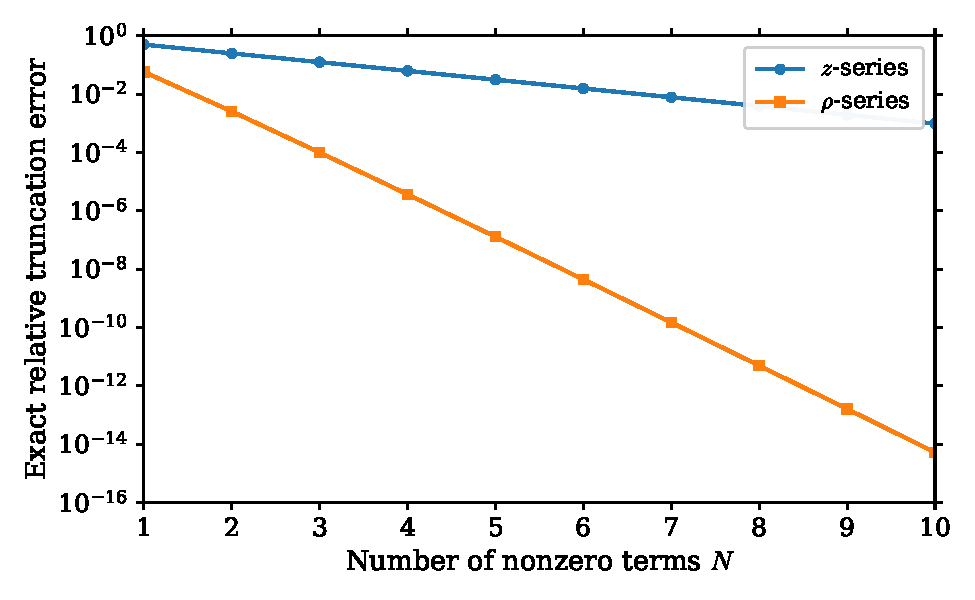
\includegraphics[width=.78\linewidth]{content/FreeElectronQuantumOptics/figures/geometry-highspin/generated/block_truncation_error.pdf}
 \caption{四维精确标量共形块 $G_{2,0}(1/2,1/2)$ 的相对截断误差。两条曲线直接由 \cref{eq:ghs-exact-block-two-tails} 计算；横轴为各自级数保留的非零项数 $N$，而不是形式上相同的径向级数幂次。}\label{fig:ghs-block-truncation-error}
\end{figure}

对于具有自旋的外算符，角向张量结构的种类还会增长，单个标量 Gegenbauer 系数便不足以描述整个块。此时可在相同的 $\rho$ 径向时间上排列有限维张量结构，并用 Casimir 关系递推其系数 \cite{ghs-costa-radial-spin}。其物理核心并没有改变：共形块依旧是一座由初级态及其全部后裔组成的圆柱能级谱。


\section{共形块的谱表示}
\label{sec:ghs-conformal-block-spectrum}


即使完全知道某个共形初级的维数和自旋，一个四点函数仍不能只由该初级贡献：必须把它的全部平移后裔一并计入。直接逐个写出所有张量分量，随级数增长会迅速变得不可管理。径向量子化的 Hilbert 空间却提供了一个与外场自旋、维度和是否存在相互作用无关的解决办法：把两对算符制备的态投影到同一个不可约共形表示中，再让尺度生成元传播这些态。


\subsection{后裔 Gram 矩阵与物理投影}

设 $\mathcal R_{\Delta,\rho}$ 是由一个标度维数为 $\Delta$、在旋转群 $SO(d)$ 下属于有限维不可约表示 $\rho$ 的初级态产生的共形表示；$\rho$ 可以是对称无迹表示，也可以是混合对称 Young 表示。其 $n$ 级后裔子空间记为 $\mathcal H_n(\mathcal R)$，其中每一个态的尺度本征值都为 $\Delta+n$。

在物理 Hilbert 空间中先模掉所有零范数后裔，然后在每一级选一组线性独立态 $|n,a\rangle$。Gram 矩阵及其逆定义为
\begin{equation}\label{eq:ghs-r4-general-level-gram}
 Q^{(n)}_{ab}=\langle n,a|n,b\rangle,\qquad
 \sum_b(Q^{(n)})^{-1}_{ab}Q^{(n)}_{bc}=\delta_{ac}.
\end{equation}
为看清为什么需要逆 Gram 矩阵，先假设一个二维子空间由两个归一化却不正交的向量 $e_1,e_2$ 张成，令 $\langle e_1,e_2\rangle=c\in\RR$ 且 $|c|<1$。直接算得
\[
 Q=\begin{pmatrix}1&c\\c&1\end{pmatrix},\qquad
 Q^{-1}=\frac1{1-c^2}\begin{pmatrix}1&-c\\-c&1\end{pmatrix}.
\]
所以
\[
 \Pi=\frac{|e_1\rangle\langle e_1|+|e_2\rangle\langle e_2|
 -c|e_1\rangle\langle e_2|-c|e_2\rangle\langle e_1|}{1-c^2}.
\]
将它作用在 $e_1$ 上，分子恰好变成 $(1-c^2)e_1$；作用在 $e_2$ 上也相同。若错误地只加两个秩一算子 $|e_a\rangle\langle e_a|$，则作用在 $e_1$ 上会多出 $c e_2$，根本不是投影。当 $c=\pm1$ 时两向量线性相关，Gram 矩阵奇异，此时须先选取独立的物理向量再求逆。这正是共形表示出现零范数后裔时的线性代数原型。

不要求 $|n,a\rangle$ 本来正交。由 \cref{eq:ghs-ope-gram-projector} 的思想，各级的正交投影为




\begin{equation}\label{eq:ghs-r4-general-projector}
 \Pi_{\mathcal R,n}=\sum_{a,b}|n,a\rangle
 (Q^{(n)})^{-1}_{ab}\langle n,b|,
 \qquad
 \Pi_{\mathcal R}=\sum_{n=0}^\infty\Pi_{\mathcal R,n}.
\end{equation}
当共形表示中的物理后裔在 Hilbert 范数意义下完备时，$\Pi_{\mathcal R}$ 是该表示闭包上的正交投影。这里的级数可以先在有限级截断、再取强算符极限；它并不是将每项当作有限矩阵后无条件直接求和。

任取由两组算符插入制备的径向态 $|\Psi_{12}\rangle$ 和 $|\Psi_{34}\rangle$，令 $t>0$ 为两组插入之间的圆柱时间距离。该表示在四点函数中的贡献，除去固定的外场运动学因子后，具有精确谱形式
\begin{align}\label{eq:ghs-r4-general-block-spectral}
 \mathcal F_{\mathcal R}(t)
 &=\langle\Psi_{34}|\Pi_{\mathcal R}\ee^{-tD}|\Psi_{12}\rangle\\
 &=\sum_{n=0}^\infty\ee^{-t(\Delta+n)}
 \sum_{a,b}\langle\Psi_{34}|n,a\rangle
 (Q^{(n)})^{-1}_{ab}\langle n,b|\Psi_{12}\rangle.
 \notag
\end{align}
式中的态还可能携带插入角度、极化或内部对称性标签；这些变量被保留在矩阵元中，因此此式不局限于四个外标量。这是共形块或多个张量结构组成的共形块矩阵的统一出发点。


在非正交后裔基中，投影必须同时使用 Gram 矩阵及其逆矩阵。
对任何基底向量 $|n,c\rangle$，利用 \cref{eq:ghs-r4-general-level-gram}，
\begin{align*}
 \Pi_{\mathcal R,n}|n,c\rangle
 &=\sum_{a,b}|n,a\rangle(Q^{(n)})^{-1}_{ab}Q^{(n)}_{bc}\\
 &=|n,c\rangle.
\end{align*}
它对该子空间的正交补为零，故 $\Pi_{\mathcal R,n}^2=\Pi_{\mathcal R,n}$，且 $\Pi_{\mathcal R,n}^\dagger=\Pi_{\mathcal R,n}$。又因为 $D|n,a\rangle=(\Delta+n)|n,a\rangle$，有
\begin{equation*}
 \Pi_{\mathcal R,n}\ee^{-tD}=\ee^{-t(\Delta+n)}\Pi_{\mathcal R,n}.
\end{equation*}
把这项关系代入完备投影的和，便直接得到 \cref{eq:ghs-r4-general-block-spectral}。如果某一级 Gram 矩阵奇异，应先去掉物理零范数方向，不能把普通逆矩阵形式地用于奇异矩阵。


对于初级态 $|\mathcal O_a\rangle$，指标 $a$ 表示 $\rho$ 的一个正交归一旋转分量，$M_{\mu\nu}$ 在此空间上有矩阵元 $(M_{\mu\nu})_{ab}$。一级态为 $P_\mu|\mathcal O_a\rangle$。使用 \cref{eq:ghs-conformal-commutators,eq:ghs-radial-generator-adjoint}，直接算得
\begin{align}\label{eq:ghs-r4-spinning-first-gram}
 Q^{(1)}_{\mu a,\nu b}
 &=\langle\mathcal O_a|K_\mu P_\nu|\mathcal O_b\rangle\\
 &=2\Delta\,\delta_{\mu\nu}\delta_{ab}
 -2(M_{\mu\nu})_{ab}.
 \notag
\end{align}
这里取 $\langle\mathcal O_a|\mathcal O_b\rangle=\delta_{ab}$；非单位的初级范数应同时乘入两项。对标量表示，$M_{\mu\nu}=0$，便恢复 \cref{eq:ghs-scalar-level-one-gram}。对更高旋转表示，一阶后裔是向量表示与 $\rho$ 的张量积，Gram 矩阵的不同旋转不可约通道一般有不同本征值。散度通道的本征值随 $\Delta-S-d+2$ 消失，正是高自旋守恒界；因此仅给每一级写一个共同的简并数是不够的。

在更高的 $n$ 级，可选择对称的 $P_{\mu_1}\cdots P_{\mu_n}|\mathcal O_a\rangle$ 作为生成集合，然后反复将所有 $K$ 向右交换。最终得到由 $\Delta$、$SO(d)$ 表示矩阵和 Kronecker 符号构成的有限 Gram 矩阵。这是一种不依赖特定 Lagrangian 的精确构造算法，也是共形块递推的代数基础。


令 $r=\ee^{-t}$，$0<r<1$。\cref{eq:ghs-r4-general-block-spectral} 把共形块写成 $r^{\Delta}$ 乘整数幂级数，但径向展开的收敛不能只用“指数衰减很快”来代替论证。设两个插入态经正的圆柱时间分离后可在 Hilbert 空间中归一，并固定 $0<t_0<t$。若将谱级数在 $n=N-1$ 后截断，则余项为
\begin{equation*}
 \mathscr R_N(t)=\langle\Psi_{34}|\sum_{n\ge N}
 \Pi_{\mathcal R,n}\ee^{-tD}|\Psi_{12}\rangle.
\end{equation*}
由于高阶子空间上的 $D\ge\Delta+N$，利用 Cauchy--Schwarz 不等式可以立即建立
\begin{align}\label{eq:ghs-r4-general-spectral-error}
 |\mathscr R_N(t)|\le{}&\ee^{-(t-t_0)(\Delta+N)}\\
 &\times\|\ee^{-t_0D/2}\Psi_{34}\|
 \;\|\ee^{-t_0D/2}\Psi_{12}\|.
 \notag
\end{align}
指数常数与表示内部的后裔简并数无关。$t_0$ 的作用是保证点状插入导致的态范数奇性已通过正时间传播处理；如果原始两态本来就正常化，可以直接取 $t_0=0$。这一不等式对任意交换旋转表示和任意外场类型成立，但前提是反射正性及所使用的径向时间顺序真实地定义了 Hilbert 空间态。洛伦兹时间解析延拓、插入点跨越 OPE 收敛圆或碰到支切时，不能直接套用此欧氏误差界。


截断误差可用谱下界与正交性直接估计。
令 $\Pi_{\ge N}=\sum_{n\ge N}\Pi_{\mathcal R,n}$。因其与 $D$ 对易，将传播因子分成三段：
\begin{equation*}
 \ee^{-tD}=\ee^{-t_0D/2}\,\ee^{-(t-t_0)D}\,\ee^{-t_0D/2}.
\end{equation*}
把两边 $\ee^{-t_0D/2}$ 吸收到 bra 与 ket 中，再对中间算符使用范数估计
\begin{equation*}
 \|\Pi_{\ge N}\ee^{-(t-t_0)D}\|
 \le\ee^{-(t-t_0)(\Delta+N)}.
\end{equation*}
最后应用 $|\langle u|A|v\rangle|\le\|u\|\|A\|\|v\|$，得到 \cref{eq:ghs-r4-general-spectral-error}。证明中从未假定各级系数非负，因此即使外场混合或共形块为张量结构矩阵，估计仍然成立。


如果外算符都是标量，但各自具有不同维数 $\Delta_i$，由四点函数中提取的距离因子与同维数情形不同。取 $x_{ij}=x_i-x_j$，并定义 $\Delta_{ij}=\Delta_i-\Delta_j$ 与交比
\begin{equation*}
 U=\frac{x_{12}^2x_{34}^2}{x_{13}^2x_{24}^2}=z\bar z,
 \qquad
 V=\frac{x_{14}^2x_{23}^2}{x_{13}^2x_{24}^2}=(1-z)(1-\bar z).
\end{equation*}
约定四点函数的外场距离因子为
\begin{align}\label{eq:ghs-r4-general-fourpoint-prefactor}
 &\langle\mathcal O_1(x_1)\mathcal O_2(x_2)
 \mathcal O_3(x_3)\mathcal O_4(x_4)\rangle\\
 &\quad=\frac{(x_{24}^2/x_{14}^2)^{\Delta_{12}/2}
 (x_{14}^2/x_{13}^2)^{\Delta_{34}/2}}
 {(x_{12}^2)^{(\Delta_1+\Delta_2)/2}
 (x_{34}^2)^{(\Delta_3+\Delta_4)/2}}\,\mathcal G(U,V).
 \notag
\end{align}
这一定义使在各个插入点处的反演权重都等于其标度维数。采用这个规范，二阶 Casimir 微分算符可以写成统一形式。令
\begin{equation}\label{eq:ghs-r4-casimir-external-weights}
 a=-\frac{\Delta_1-\Delta_2}{2},\qquad
 b=\frac{\Delta_3-\Delta_4}{2},\qquad
 \nu=\frac{d-2}{2}.
\end{equation}
定义
\begin{align}\label{eq:ghs-r4-casimir-general-d}
 \mathcal D_{a,b}^{(d)}
 &=\mathcal D_z^{(a,b)}+\mathcal D_{\bar z}^{(a,b)}
 +2\nu\frac{z\bar z}{z-\bar z}
 \bigl[(1-z)\partial_z-(1-\bar z)\partial_{\bar z}\bigr],\\
 \mathcal D_w^{(a,b)}
 &=w^2(1-w)\partial_w^2-(a+b+1)w^2\partial_w-abw.
 \notag
\end{align}
那么交换对称无迹自旋 $S$、维数 $\Delta$ 的共形块满足
\begin{equation}\label{eq:ghs-r4-casimir-general-eq}
 \mathcal D_{a,b}^{(d)}G_{\Delta,S}^{a,b}(z,\bar z)
 =\frac12\bigl[\Delta(\Delta-d)+S(S+d-2)\bigr]
 G_{\Delta,S}^{a,b}(z,\bar z).
\end{equation}
这条方程给出一般 $d$ 维、四个任意维数标量外场的共形块，而不要求每一种维数都有已知的初等超几何闭式解。令 $a=b=0$ 就恢复 \cref{eq:ghs-casimir-differential-operator}。要得到唯一的物理块，仍必须指定相应通道的 OPE 边界条件。若外场自身带自旋，Casimir 不再只作用于一个标量函数，而是作用于若干独立张量结构组成的矩阵值函数；此时 \cref{eq:ghs-r4-general-block-spectral} 是比单个微分方程更稳健的起点 \cite{ghs-dolan-osborn,ghs-costa-radial-spin,ghs-hogervorst}。


对两个不相同的广义自由标量 $A,B$，双粒子态不只包含前文构造的最低扭度 $n=0$ 家族。在去除总平移后裔的独立双体扇区中，还出现
\begin{equation}\label{eq:ghs-r4-generalized-free-doubletrace}
 [AB]_{n,S},\qquad
 \Delta_{n,S}=\Delta_A+\Delta_B+2n+S,
 \qquad n,S\in\NN_0.
\end{equation}
这里 $n$ 计数两粒子相对运动中的径向激发；可以在双体导数多项式空间内按旋转表示和共形 $K_\mu$ 约束逐级正交化，构造相应初级态。$n=0$ 的闭式解就是 \cref{eq:ghs-r4-mixed-primary-coefficients}，其系数见 \cref{eq:ghs-r4-mft-leading-ope}；$n>0$ 的归一化则需要更高导数阶数的 Gram 矩阵。相同实标量的相同粒子交换还要求 $S$ 为偶数。若标量恰好饱和自由场幺正性界，运动方程会进一步产生零范数关系，因而不能把广义自由长表示的全部 $n$ 家族原样保留为独立物理初级。

对于真正相互作用的幺正共形场论，\cref{eq:ghs-r4-generalized-free-doubletrace} 不是每个有限 $S$ 的精确谱定理。一般只能把具有适当谱条件的高自旋家族写作
\begin{equation}\label{eq:ghs-r4-interacting-doubletwist}
 \Delta_{n,S}=\Delta_A+\Delta_B+2n+S+\gamma_{n,S},
\end{equation}
并在可控制的光锥大自旋极限中研究 $\gamma_{n,S}$ 的衰减。是否存在给定 $n$ 的家族、允许哪些内部对称性通道，以及极限如何趋近广义自由数据，均由实际的交叉对称方程决定。无限自旋极限的存在并不替代一个具体相互作用理论中有限自旋 OPE 数据的计算。

由此，径向量子化提供了两个互补的精确入口。若模型具备广义自由因子化，可把高自旋初级、范数和最低扭度系数直接算到底；若只有共形对称和单位性，则使用 Gram 投影与 Casimir 方程保留全部后裔的普适结构。把这两种入口区分开，才能在使用大自旋近似时准确知道哪些是代数定理，哪些是某个模型的动力学输入。


有限自旋共形块的解析形式已经确定，但交叉对称还会约束无限自旋族的累积行为。由此产生的大自旋极限必须同时控制交比与自旋的缩放。


前面自由标量双粒子态的总维数精确等于 $2\delta+S$。如果把它放入相互作用理论，什么量能够延续？单粒子振子模式、两体位置振幅和 Wick 配对通常都不再存在；但自旋 $S$、标度维数 $\Delta$ 及扭度 $\tau=\Delta-S$ 仍是定义良好的共形量子数。由交叉对称控制的大自旋展开，正是对这些普适量所做的计算。


设 $\mathcal X$ 是标度维数为 $\Delta_\mathcal X$ 的标量初级算符。在忽略相互作用的广义自由极限中，两个 $\mathcal X$ 可以组成总自旋 $S$ 的对称无迹双算符；除了分配给自旋的 $S$ 个未收缩导数，还允许 $2n$ 个相对导数发生收缩。算符的形式可以写为
\begin{equation}\label{eq:ghs-double-twist-operator}
 [\mathcal X\mathcal X]_{n,S}
 \sim\mathcal X\,\partial_{(\mu_1}\cdots\partial_{\mu_S)}(\partial^2)^n\mathcal X
 +\text{初级投影所需的其他项},
\end{equation}
其中括号表示对称并去迹。这不是一个已经完成初级投影的定义式，因为导数须重新分配到两个因子上，且要减掉总导数后裔。它明确显示两个标签的意义：$S$ 控制总角动量，$n$ 控制附加的相对激发。广义自由极限的维数为
\begin{equation}\label{eq:ghs-double-twist-tower}
 \Delta_{n,S}^{(0)}=2\Delta_\mathcal X+2n+S,
 \qquad \tau_{n,S}^{(0)}=2\Delta_\mathcal X+2n.
\end{equation}
如果两个外算符相同且为玻色标量，交换两个因子要求 $S$ 为偶数；对不同外算符则无此限制。

把这个结果与 \cref{eq:ghs-spin-energy} 对照可以看出自由局域标量的特殊之处：$\Delta_\chi=\delta$，于是 $n=0$ 的整塔恰好落在 $d-2$ 的幺正性边界。但是 $\chi$ 自身满足 $\partial^2\chi=0$，因此 $n>0$ 的形式表达式可能成为后裔、零范数或与较低算符等价。不能把广义自由场中所有 $n$ 的算符不加筛选地搬到严格自由标量 Hilbert 空间。


把相互作用强度统称为无量纲参数 $g$。给定重整化方案中的一个可以连续追踪的双扭度初级算符，其维数允许写成
\begin{equation}\label{eq:ghs-doubletwist-anomalous-dimension}
 \Delta_{n,S}(g)=2\Delta_\mathcal X(g)+2n+S+\gamma_{n,S}(g).
\end{equation}
这里 $\gamma_{n,S}$ 定义的是相对于两个外标量真实维数之和的附加结合效应，而不是相对于它们的裸经典维数。这样定义可以把单粒子场重整化与真正的两体效应区分开。当多个初级算符具有相同对称性和相近维数时，应先对混合矩阵对角化，再为其本征态赋予 $\gamma_{n,S}$。

一旦 $\gamma_{n,S}\neq0$，则圆柱能量改变 $\Delta E_{n,S}=\hbar c\,\gamma_{n,S}/R$。这是由态—算符对应得到的严格能量差，但不能把 $\gamma_{n,S}$ 直接理解成平直空间两粒子束缚能：圆柱没有平直时空粒子散射的渐近出入态，其尺度 $R$ 也是共形映射所选择的量。


高自旋展开经常用共形自旋而不是裸的整数 $S$ 来组织。对近似双扭度初级态，可定义
\begin{equation}\label{eq:ghs-conformal-spin}
 \mathcal J_{n,S}^2
 =\left(S+n+\Delta_\mathcal X\right)
 \left(S+n+\Delta_\mathcal X-1\right).
\end{equation}
它是双扭度族的主阶共形自旋平方；考虑反常维数后的精确本征值须把相应的半扭度修正纳入。$S\to\infty$ 时 $\mathcal J_{n,S}=S+O(1)$，因此 $1/S$ 与 $1/\mathcal J$ 有相同的领先量级，却在次领先阶给出不同系数。

若某一最低非单位交叉通道初级算符的扭度为 $\tau_*>0$，它对固定 $n$ 的双扭度反常维数常给出
\begin{equation}\label{eq:ghs-large-spin-gamma-scaling}
 \gamma_{n,S}
 =\frac{A_n}{\mathcal J_{n,S}^{\tau_*}}
 +o\!\left(\mathcal J_{n,S}^{-\tau_*}\right).
\end{equation}
$A_n$ 由外算符—交换算符的 OPE 系数及自旋张量结构决定；其符号与适用范围不能仅凭量纲判定。若有多个同扭度交换、简并混合、对数增强或其他交叉通道奇异性，应将相应贡献一起处理。一般定理支持大自旋双扭度谱的存在；\cref{eq:ghs-large-spin-gamma-scaling} 的单幂首项则需要最低扭度交换确实主导的条件，见 \cite{ghs-komargodski,ghs-caronhuot}。


\cref{eq:ghs-free-scalar-fourpoint} 在 $z\to0$ 时可以重写为
\begin{equation}\label{eq:ghs-free-lightcone-limit}
 \mathcal G_\chi(z,\bar z)
 =1+(z\bar z)^\delta
 +\frac{(z\bar z)^\delta}{[(1-z)(1-\bar z)]^\delta}.
\end{equation}
如果在 $z\to0$ 的同时让 $\bar z\to1$，第三项含有 $z^\delta(1-\bar z)^{-\delta}$ 的增强因子。这个双尺度结构不是固定少数个共形块便能够在所有角度区间内一致重建的；在某一通道有限截断自旋后，再取交叉通道的极端极限可能不交换。完整的共形块展开必须允许一座向任意大自旋延伸的谱塔。

这里可以看清两类大自旋极限的联系与差别。前面 $S\to\infty$ 时 $|z_1-z_2|^S$ 出现对径峰，是\emph{特定自由场三点矩阵元的空间鞍点现象}；光锥自举中的 $S\to\infty$ 则来自\emph{不同 OPE 通道必须重建相同四点函数的解析约束}。二者都由高自旋表示控制，但它们是不同的可观测对象，也不共享一个无条件的“对径粒子运动”图像。


Lorentz 型反演公式利用解析延拓后的四点函数双不连续部分（通常记作 $\operatorname{dDisc}$），恢复随自旋解析变化的 OPE 数据。在合适的 Regge 有界条件和收敛自旋范围内，该方法能将交叉通道信息组织为共形块系数的积分表示，并使大共形自旋的系统展开变得明确，参见 \cite{ghs-caronhuot}。

反演公式的输入是经过规范化的四点函数及其解析结构，输出是谱极点和 OPE 系数；它并不能仅从一个自由场双粒子振幅预测某个相互作用 CFT 的反常维数。要把 \cref{eq:ghs-large-spin-gamma-scaling} 的 $A_n$ 算成具体数字，必须再给出交换算符的维数、三点函数数据和所选共形块约定。


无论在自由场还是相互作用场论里，$S$ 都是旋转群表示的标签，决定了某个共形初级态的角动量。它不是一颗基本粒子必须拥有的内禀自旋。对于自由标量双线性流，$S$ 来自两个无自旋基本量子及其相对导数；对于规范理论的单迹高自旋算符，$S$ 也可能来自共变导数沿光锥方向的分配。两类高自旋的算符代数、混合矩阵、反常维数甚至 Hilbert 空间粒子解释都可能不同，不能因为标度维数都大就视为同一类态。

一个可执行的相互作用研究因而应同时说明三个问题：选中的高自旋初级算符属于哪个全局对称性及混合扇区；它的真实 $\Delta_S$ 由怎样的重整化群或自举数据确定；研究的实验或数学可观测量是四点函数、谱密度、算符矩阵元还是理想化球面探测概率。只有明确这些对象，才有可能把自由场的精确计算推广为可信的场论结论。


欧氏共形块的径向展开在收敛域内提供精确表达。若让两个插入点接近光锥，同时取交换自旋很大，就必须重新安排极限次序；这正是从有限自旋的对数奇性过渡到无限塔幂律奇性的原因。


交叉对称要求同一个四点函数能够沿不同的配对顺序展开。若只让两个点在欧氏空间中靠近，固定有限个初级表示的贡献都容易控制；困难出现在两个通道同时逼近各自的奇异边界。这时越来越高的自旋能够抵消越来越小的角距离，因而不能事先固定自旋再取极限。要理解双扭度谱为何出现，必须先看清共形块在双尺度区域中的真实函数形状。


仍取四维相同标量的约定，令 $z\to0$ 且 $0<\bar z<1$ 固定。初级算符的扭度 $\tau=\Delta-S$ 已由 \cref{eq:ghs-twist-definition} 定义，幺正性要求 $S\ge1$ 时 $\tau\ge2$。把 \cref{eq:ghs-four-dimensional-exact-block} 的两项分别展开，$k_{\Delta+S}(z)$ 比 $k_{\Delta-S-2}(z)$ 多出 $z^{S+1}$，得到
\begin{equation}\label{eq:ghs-lightcone-fixed-spin-block}
 G_{\Delta,S}(z,\bar z)
 =\frac{z^{\tau/2}}{2^S}k_{\Delta+S}(\bar z)
 +O\bigl(z^{\tau/2+1}\bigr),
 \qquad z\to0,\quad \bar z\ \text{固定}.
\end{equation}
这里的余项允许依赖 $\bar z,\Delta,S$；不能认为它对 $S\to\infty$ 仍一致有界。\cref{eq:ghs-lightcone-fixed-spin-block} 展示了扭度的物理意义：在光锥极限中控制 $z$ 幂次的是 $\Delta-S$，而自旋对剩余的 $\bar z$ 依赖仍然重要。


\begin{proof}
设 $h_+=(\Delta+S)/2$、$h_-=(\Delta-S-2)/2$。根据超几何级数首项，
\begin{equation*}
k_{\Delta+S}(z)=z^{h_+}[1+O(z)],\qquad
k_{\Delta-S-2}(z)=z^{h_-}[1+O(z)].
\end{equation*}
对固定的 $\bar z>0$，预因子满足 $z\bar z/(z-\bar z)=-z[1+O(z)]$。于是反对称括号中第二项主导，整个表达式的首项为
\begin{align*}
&\frac1{2^S}(-z)\left[-k_{\Delta+S}(\bar z)
z^{(\tau-2)/2}\right]\bigl[1+O(z)\bigr]\\
&\qquad=\frac{z^{\tau/2}}{2^S}k_{\Delta+S}(\bar z)
\bigl[1+O(z)\bigr].
\end{align*}
这说明 \cref{eq:ghs-lightcone-fixed-spin-block} 不是从自由场经验类推而来，而是四维 Casimir 精确解的受控固定自旋渐近。
\end{proof}

若 $\bar z\to1$，令 $y=1-\bar z\to0^+$。函数 $k_{2h}(1-y)$ 可用 Euler 积分表示为
\begin{equation}\label{eq:ghs-lightcone-k-euler}
 k_{2h}(1-y)=\frac{\Gamma(2h)}{\Gamma(h)^2}(1-y)^h
 \int_0^1\frac{[t(1-t)]^{h-1}}{[1-(1-y)t]^h}\,\dd t,
 \qquad h>0.
\end{equation}
这个积分有两个竞争的尺度：$h$ 控制积分核的陡峭程度，$y$ 控制端点附近分母何时变小。取 $h\to\infty$、$y\to0$，同时让 $\xi=2h\sqrt y$ 保持有限，则积分局部化后由第二类修正贝塞尔函数 $K_0(\xi)$ 描述：
\begin{equation}\label{eq:ghs-lightcone-k-bessel}
 k_{2h}(1-y)\sim
 \frac{2\Gamma(2h)}{\Gamma(h)^2}K_0(2h\sqrt y),
 \qquad h\gg1,\quad h\sqrt y=O(1).
\end{equation}
这是一个联合极限，而不是在任意 $y$ 处都准确的全局近似。特别地，$h\sqrt y=O(1)$ 表明对 $S\sim2h\to\infty$，重要角区宽度为 $y=O(S^{-2})$。因此先令 $S$ 固定再送 $y\to0$，与让 $S\sqrt y$ 固定的极限有不同结果。


\begin{proof}
在 \cref{eq:ghs-lightcone-k-euler} 令 $t=1-a/h$，并固定 $a>0$。当 $h\to\infty$ 且 $y=\xi^2/(4h^2)$ 时，核中的主要指数可写为
\begin{equation*}
\left[\frac{t(1-t)}{1-(1-y)t}\right]^h
=\exp\left[-a-\frac{h^2y}{a}+o(1)\right]
\end{equation*}
乘以测度与缓变因子后，主导端点积分按 $a$ 化为
\begin{equation*}
\int_0^\infty\frac{\dd a}{a}
\exp\left[-a-\frac{h^2y}{a}\right]
=2K_0(2h\sqrt y).
\end{equation*}
最后一式来自 $K_0(2\sqrt q)=\tfrac12\int_0^\infty a^{-1}\ee^{-a-q/a}\dd a$。结合 Euler 积分的规范化便得到 \cref{eq:ghs-lightcone-k-bessel}。取 $y\to0$ 的另一条核对途径是比较两边的对数奇性：
\begin{align*}
k_{2h}(1-y)&\sim\frac{\Gamma(2h)}{\Gamma(h)^2}
\left[-\log y+2\psi(1)-2\psi(h)\right],\\
2K_0(2h\sqrt y)&\sim-\log y-2\log h-2\gamma_{\rm E}.
\end{align*}
由于 $\psi(h)=\log h+O(h^{-1})$，二者的首项一致。端点替换需在 $a=0$ 和 $a=\infty$ 外做一致余项控制，故这里所写的是固定 $\xi>0$ 的领先渐近，而不是包含 $\xi=0$ 的统一误差界。
\end{proof}

\begin{figure}[htbp]
\centering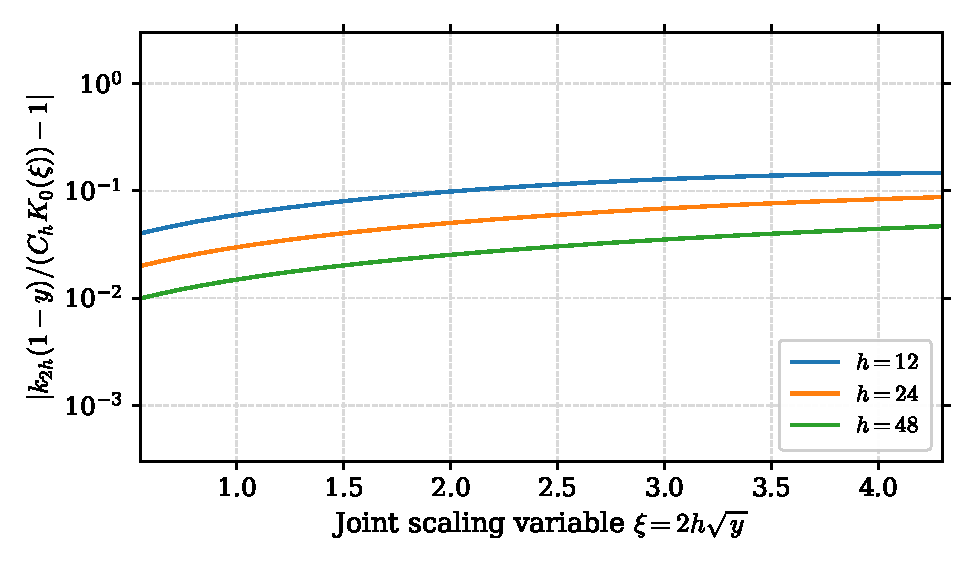
\includegraphics[width=.79\linewidth]{content/FreeElectronQuantumOptics/figures/geometry-highspin/generated/lightcone_bessel_error.pdf}
\caption{在联合极限 $y=[\xi/(2h)]^2$ 下，精确超几何核 $k_{2h}(1-y)$ 与 $[2\Gamma(2h)/\Gamma(h)^2]K_0(\xi)$ 的相对误差。较大 $h$ 的误差系统下降，验证边界层近似而非固定 $y$ 近似。}\label{fig:ghs-lightcone-bessel-error}
\end{figure}

\cref{fig:ghs-lightcone-bessel-error} 只比较共形块的特定超几何因子；它不是对完整相互作用 CFT 的数值拟合，也不能取代离散高自旋谱的求和控制。


考虑一个明确可计算的模型：高自旋谱密度在连续近似下为 $h^{p-1}$，其中 $p>0$。把单个大自旋块的贝塞尔核心看成 $K_0(2h\sqrt y)$，那么
\begin{equation}\label{eq:ghs-large-spin-bessel-integral}
 \int_0^\infty h^{p-1}K_0(2h\sqrt y)\,\dd h
 =\frac{\Gamma(p/2)^2}{4\,y^{p/2}}.
\end{equation}
右侧在 $y\to0^+$ 发散，而任何固定 $h$ 的核最多只有对数发散。强幂次奇异性恰恰由无界自旋区 $h\sim y^{-1/2}$ 集体贡献。


\begin{proof}
令 $q=\sqrt y$，利用
\begin{equation*}
K_0(2qh)=\frac12\int_0^\infty\frac{\dd t}{t}
\ee^{-t-q^2h^2/t},\qquad h,q,t>0.
\end{equation*}
由于被积函数非负，可以交换积分次序：
\begin{align*}
&\int_0^\infty h^{p-1}K_0(2qh)\dd h\\
&\quad=\frac12\int_0^\infty\frac{\dd t}{t}\ee^{-t}
\int_0^\infty h^{p-1}\ee^{-q^2h^2/t}\dd h\\
&\quad=\frac{\Gamma(p/2)}4q^{-p}
\int_0^\infty t^{p/2-1}\ee^{-t}\dd t\\
&\quad=\frac{\Gamma(p/2)^2}{4q^p}
=\frac{\Gamma(p/2)^2}{4y^{p/2}}.
\end{align*}
最后一次积分即 Gamma 函数定义。该恒等式本身是精确的；在实际共形块中把离散自旋和与 OPE 系数换成这个连续权重，需要额外验证大自旋谱密度、块归一化及误差，因此不能把 $p$ 任意代入就声称得到具体 CFT 的临界指数。
\end{proof}

交叉通道不仅决定领先奇异性，还决定反常维数如何随自旋改变。设某类算符的扭度为 $\tau=\tau_0+\gamma$，则其贡献中的一项满足
\begin{equation}\label{eq:ghs-twist-log-expansion}
 U^{\tau/2}=U^{\tau_0/2}
 \left[1+\frac\gamma2\log U+\frac{\gamma^2}{8}(\log U)^2+O(\gamma^3)\right].
\end{equation}
当在洛伦兹运动学中绕过分支点，$\log U$ 会增加或减少 $2\pi\ii$。两种绕行方式的平均值可以从欧氏原函数中剥离掉，使多重不连续性成为提取交换数据的有力工具。

为了看清该操作，考虑 $y>0$ 处的复函数 $f_\alpha(y)=y^\alpha$，并把绕 $y=0$ 一周后的解析延拓分别写为 $f_\alpha^{\circlearrowleft}=\ee^{2\pi\ii\alpha}f_\alpha$、$f_\alpha^{\circlearrowright}=\ee^{-2\pi\ii\alpha}f_\alpha$。在相同标量的零附加相位约定中，定义
\begin{equation}\label{eq:ghs-ddisc-definition}
 \operatorname{dDisc}[f]
 =f-\frac12f^{\circlearrowleft}-\frac12f^{\circlearrowright}.
\end{equation}
于是
\begin{equation}\label{eq:ghs-ddisc-power}
 \operatorname{dDisc}[y^\alpha]
 =2\sin^2(\pi\alpha)y^\alpha.
\end{equation}
令 $\alpha\to0$，逐项比较该式的 Taylor 系数，得到
\begin{equation}\label{eq:ghs-ddisc-log-check}
 \operatorname{dDisc}[1]=0,\qquad
 \operatorname{dDisc}[\log y]=0,\qquad
 \operatorname{dDisc}[(\log y)^2]=4\pi^2.
\end{equation}
它说明，当支切指数围绕整数值作小扰动时，双不连续性首次感受到指数变化的阶数可能是二阶。但若原有幂次非整数，或外部算符维数带来额外绕行相位，阶数会不同；\cref{eq:ghs-ddisc-log-check} 不能被误读成任何 CFT 的一圈修正都没有双不连续性。

真正的洛伦兹反演公式还包含明确的积分测度、共形核和 Regge 有界性条件。它把交叉通道的双不连续性转换成随自旋解析变化的 OPE 数据，并通过谱极点提取 $\Delta_{n,S}$。这一精确公式的建立需要重新处理洛伦兹区的积分轮廓，不能仅凭 \cref{eq:ghs-ddisc-definition} 代替；其全面形式见 \cite{ghs-caronhuot,ghs-alday-large-spin}。在上述计算中，\cref{eq:ghs-lightcone-fixed-spin-block,eq:ghs-large-spin-bessel-integral,eq:ghs-ddisc-power} 分别解释了扭度的光锥幂次、无穷自旋的集体增强和反常维数产生的分支信息。




\section{相互作用、表示重组与反常维数}
\label{sec:ghs-higher-spin-conservation}


无限多个高自旋守恒流是自由场的强约束。加入相互作用后，哪些守恒律还能保持，哪些后裔会重新成为物理态？这个问题可以不依靠一个完整可解的相互作用模型，而从局域运动方程、两点函数和径向范数出发，先求出守恒律破缺与反常维数之间的逻辑关系。


为了能显式写出算符方程，考虑四维附近的一个实标量模型，欧氏作用量取
\begin{equation}\label{eq:ghs-phi4-action}
 \mathscr I_g[\varphi]=\int\dd^d x\left[
 \frac12(\partial_\mu\varphi)^2
 +\frac{\mu_{\mathrm R}^{\epsilon}g}{4!}\varphi^4\right],
 \qquad d=4-\epsilon.
\end{equation}
其中 $\mu_{\mathrm R}$ 是重整化尺度，$g$ 是无量纲重整化耦合常数。此处公式用来展示微扰理论的局域结构；一般 $g\neq0$ 时不能先假定该模型恰是 CFT。只有在满足 $\beta(g_*)=0$ 的临界不动点，才可以将算符组织为相互作用共形初级表示。

忽略接触项和算符重整化暂时引入的细节，作用量变分得到经典运动方程
\begin{equation}\label{eq:ghs-phi4-eom}
 \partial^2\varphi=\frac{\mu_{\mathrm R}^\epsilon g}{3!}\varphi^3.
\end{equation}
在自由理论，右侧为零，正是前面高自旋守恒流成立的关键。当 $g\ne0$，对由多个导数组成的高自旋流求散度时，运动方程会将一部分项变成包含三个或更多场的复合算符。因而对 $S>2$ 的一般高自旋流，有形式
\begin{equation}\label{eq:ghs-broken-higher-spin-current}
 \partial^{\mu_1}J^{(S)}_{\mu_1\cdots\mu_S}
 =g\,\mathcal K^{(S-1)}_{\mu_2\cdots\mu_S}+O(g^2),
\end{equation}
其中 $\mathcal K^{(S-1)}$ 是与选定理论和重整化方案有关的复合算符；式中的 $g$ 已把合适的 $\mu_{\mathrm R}^\epsilon$ 因子吸收到 $\mathcal K$ 的约定中。此式只陈述弱耦合下可连续追踪的高自旋流的局域非守恒关系，不给未经计算的 $\mathcal K$ 系数。


对任意幺正共形场论 的一阶矢量初级算符 $J_\mu$，设其二点函数为
\begin{equation}\label{eq:ghs-vector-two-point}
 \langle J_\mu(x)J_\nu(0)\rangle
 =\frac{C_J}{(x^2)^\Delta}
 I_{\mu\nu}(x),\qquad
 I_{\mu\nu}(x)=\delta_{\mu\nu}-2\frac{x_\mu x_\nu}{x^2}.
\end{equation}
$C_J>0$ 是选定张量归一化后的二点函数系数。利用 $\partial_\mu x^\mu=d$ 和 $x^\mu I_{\mu\nu}=-x_\nu$，可直接求一次散度：
\begin{equation}\label{eq:ghs-vector-divergence-identity}
 \partial_x^\mu\langle J_\mu(x)J_\nu(0)\rangle
 =2C_J(\Delta-d+1)\frac{x_\nu}{(x^2)^{\Delta+1}}.
\end{equation}
若 $\Delta=d-1$，相关函数在非重合点处严格横向。这不是自旋一偶然出现的代数巧合，而是短表示散度后裔范数为零在位置空间的对应物。



\begin{proof}
先直接计算张量求导
\begin{align*}
\partial_x^\mu I_{\mu\nu}(x)
&=-2\partial_x^\mu\frac{x_\mu x_\nu}{x^2}
=-2(d-1)\frac{x_\nu}{x^2},\\
I_{\mu\nu}(x)\partial_x^\mu(x^2)^{-\Delta}
&=-2\Delta(x^2)^{-\Delta-1}x^\mu I_{\mu\nu}
=2\Delta\frac{x_\nu}{(x^2)^{\Delta+1}}.
\end{align*}
两项相加即为 \cref{eq:ghs-vector-divergence-identity}。第二个插入点 $y$ 的导数在平移不变的函数上满足 $\partial_y=-\partial_x$，因此
\begin{align*}
&\langle(\partial\cdot J)(x)(\partial\cdot J)(0)\rangle\\
&=-2C_J(\Delta-d+1)\partial_x^\nu
\left[\frac{x_\nu}{(x^2)^{\Delta+1}}\right]\\
&=2C_J(\Delta-d+1)(2\Delta+2-d)
\frac1{(x^2)^{\Delta+1}},\qquad x\ne0.
\end{align*}
这里 $x=0$ 的接触项需要单独进行分布论处理，不参与非重合点两点函数的比较。
\end{proof}

现在取 $\Delta=d-1+\gamma_1$，得到
\begin{equation}\label{eq:ghs-vector-divergence-gamma}
 \langle(\partial\cdot J)(x)(\partial\cdot J)(0)\rangle
 =2C_J\gamma_1(d+2\gamma_1)
 (x^2)^{-d-\gamma_1}.
\end{equation}
只要 $\gamma_1>0$，散度态取得非零范数。高自旋 $S>1$ 的相应张量公式带有依赖 $S,d$ 与投影约定的正系数，但在幺正界附近都含有 $\Delta_S-(S+d-2)$ 这一线性因子。由此可以通过计算非守恒算符的二点函数，间接确定高自旋反常维数。


在一个存在连续弱耦合共形固定点的模型中，假设自由流 $J_S^{(0)}$ 的散度严格为零，而破缺方程起始于 $\partial\cdot J_S=g\mathcal K_S+O(g^2)$。两边的二点函数在领先阶满足
\begin{equation}\label{eq:ghs-broken-current-norm-scaling}
 \langle(\partial\cdot J_S)(x)(\partial\cdot J_S)(0)\rangle
 =g^2\langle\mathcal K_S(x)\mathcal K_S(0)\rangle_{g=0}
 +O(g^3).
\end{equation}
另一方面，共形二点函数的张量求导必含 $\gamma_S=\Delta_S-(S+d-2)$。若右侧自由理论的 $\mathcal K_S$ 具有有限非零范数、没有导致阶数改变的混合或额外小参数，便得到
\begin{equation}\label{eq:ghs-broken-current-gamma-order}
 \gamma_S=O(g^2).
\end{equation}
这个推理说明量级来自两次非守恒插入，并未计算出 $g^2$ 的数值系数。若相互作用本身已经使算符在一阶混合，或所讨论的流不是自由理论的守恒短表示，就不能用这一估计。对于四维附近的 Wilson--Fisher 固定点，$g_*=O(\epsilon)$，因此典型非保护高自旋流的维数偏移从 $O(\epsilon^2)$ 开始；真正数值系数仍须进行算符重整化或非守恒二点函数计算。


平移不变性保证存在经适当改进及重整化的应力张量 $T_{\mu\nu}$，其局域 Ward 恒等式使 $\partial^\mu T_{\mu\nu}$ 在非重合相关函数中为零。在幺正共形固定点，其标度维数被保护为 $\Delta_T=d$。因此 $S=2$ 时
\begin{equation}\label{eq:ghs-stress-tensor-protection}
 \Delta_T=d,
 \qquad\gamma_T\equiv\Delta_T-(d-2+2)=0.
\end{equation}
这与通常的 $S=4,6,\ldots$ 高自旋流可以获得 $\gamma_S>0$ 形成鲜明对比。若自旋一流是精确内部全局对称性的 Noether 流，它的维数同样由 $\Delta_{J_1}=d-1$ 保护。某种流是否守恒，最终取决于真实的对称性及其 Ward 恒等式，而不是它包含的导数数目。


某个高自旋流若精确守恒，其表面荷不仅改变局域算符，还会对更高相关函数施加强 Ward 恒等式。不同高自旋荷之间的闭合关系可迫使更多高自旋流存在，在适当条件下甚至固定一整类相关函数。已知的三维高自旋约束定理表明：在特定单位性、唯一应力张量与相关谱条件下，一个自旋大于二的守恒流会使应力张量及高自旋流相关函数具有自由场结构，参见 \cite{ghs-maldacena-zh,ghs-alba-diab}。这些结论的维数及附加假设很重要，不能简单升级成“任何理论中出现一条守恒高自旋流就意味着所有自由度都不相互作用”。

若高自旋对称性仅在大 $N$ 理论中近似成立，则流的散度和反常维数可以按 $1/N$ 系统组织；一些三维 Chern--Simons 物质理论就是这种研究范式，参见 \cite{ghs-maldacena-zh-broken}。此时“近似守恒”是有控制参数的近似，而不仅是声称高自旋荷受到微小破坏。


共形场论与反德西特空间之间的谱对应把边界初级维数和自旋映射到体场的质量、能级和旋转表示。若某个高自旋流的维数恰好饱和守恒界，体对偶中往往对应具有规范冗余的无质量高自旋场；当该维数离开幺正界，相应表示改变。这个联系有严格的表示论基础，但具体的体理论及其相互作用不能仅由本讲义的自由标量 Fock 态构造决定。讨论高自旋引力、弦谱或高能散射时还需要补充大 $N$、谱隙、单迹算符等假设。

自由高自旋双粒子态最稳定的贡献，是提供了一套可逐式核验的短表示基准：在这个基准上，能量、三点函数、双体矩阵元、单体模式谱以及大自旋渐近都能显式计算。加入相互作用以后，这些对象有的保持纯粹运动学定义，有的必须重新由 CFT 数据或重整化决定。沿着二点函数—三点函数—四点函数的顺序逐步替换自由计算，才是从特殊模型通向一般高自旋量子场论的可靠路径。


\subsection{内部对称性与奇自旋流}

单个实标量只产生偶数自旋双线性初级态，并不意味着自由场中不存在奇自旋守恒流。真正使奇自旋算符消失的，是两个场既为玻色子、又属于同一物理分量的交换对称性。引入多个场分量以后，同一个共形初级递推式便可以同时产生偶数与奇数自旋，而且奇自旋的最低例子正是熟悉的内部对称性 Noether 流。


设 $\varphi^a(x)$，$a=1,\ldots,N$，为 $N$ 个彼此独立的无质量实标量场，欧氏作用量
\begin{equation}\label{eq:ghs-flavor-free-action}
 \mathscr I_N=\frac12\sum_{a=1}^N\int\dd^d x\,(\partial_\mu\varphi^a)^2,
 \qquad\langle\varphi^a(x)\varphi^b(0)\rangle
 =\delta^{ab}\frac{C_d}{|x|^{2\delta}}.
\end{equation}
所有场的球谐能量都是 $\ell+\delta$，但每个球谐模式多了一个内部指标，产生算符满足
\begin{equation}\label{eq:ghs-flavor-fock-commutator}
 [b_{k,a},b_{j,b}^\dagger]=\delta_{kj}\delta_{ab},
 \qquad[b_{k,a},b_{j,b}]=0.
\end{equation}
这里 $a$ 是内部对称性标签，不是球面的简并指标；$k$ 仍表示前面固定复极化方向的最高权模式。


沿用 \cref{eq:ghs-primary-coefficients} 中的系数，定义带两个内部指标的双线性算符
\begin{equation}\label{eq:ghs-flavor-high-spin-bilinear}
 J_S^{ab}(x;\vb\varepsilon)=
 \sum_{k=0}^S c_k:
 (D_+^k\varphi^a)(D_+^{S-k}\varphi^b):(x).
\end{equation}
由 $c_{S-k}=(-1)^S c_k$ 和玻色正规序交换性，直接更换求和指标 $k\mapsto S-k$，有
\begin{equation}\label{eq:ghs-flavor-exchange-parity}
 J_S^{ba}=(-1)^S J_S^{ab}.
\end{equation}
因此偶数自旋属于内部指标的对称张量，奇数自旋属于反对称张量。对偶数 $S$，$J_S^{ab}$ 还可分成迹 $\delta_{ab}J_S^{ab}$ 与对称无迹部分；对奇数 $S$，只有反对称内部表示。

如果强制 $a=b$，那么 \cref{eq:ghs-flavor-exchange-parity} 在奇数 $S$ 时给出 $J_S^{aa}=-J_S^{aa}=0$。这正是原先单个实标量结果的完整原因，而不是一般场论中对奇自旋的禁戒定理。


取 $S=1$，由 $c_0=1$、$c_1=-1$，
\begin{equation}\label{eq:ghs-flavor-spin-one-current}
 J_1^{ab}(x;\vb\varepsilon)
 =:\!\varphi^aD_+\varphi^b-\varphi^bD_+\varphi^a\!:.
\end{equation}
恢复任意方向的矢量指标，得到
\begin{equation}\label{eq:ghs-on-current}
 j_\mu^{ab}=:\!\varphi^a\partial_\mu\varphi^b-\varphi^b\partial_\mu\varphi^a\!:.
\end{equation}
它满足 $j_\mu^{ab}=-j_\mu^{ba}$。直接求散度：
\begin{align*}
 \partial^\mu j_\mu^{ab}
 &=:\!(\partial^\mu\varphi^a)(\partial_\mu\varphi^b)
 +\varphi^a\partial^2\varphi^b\\
 &\qquad-(\partial^\mu\varphi^b)(\partial_\mu\varphi^a)
 -\varphi^b\partial^2\varphi^a\!:\\
 &=:\!\varphi^a\partial^2\varphi^b-\varphi^b\partial^2\varphi^a\!:=0.
\end{align*}
其中第一与第三项直接相消，第二与第四项由各分量的自由运动方程消失。这个流的维数为 $d-1$，正好饱和 \cref{eq:ghs-spin-unitarity-bound-extended} 的自旋一界。它也是自由 $O(N)$ 内部旋转对称性的 Noether 流。


对原始场作跨顶点 Wick 收缩，定义 $W_i=(\vb\varepsilon\cdot x_i)/|x_i|^2$，得到
\begin{align}\label{eq:ghs-flavor-threepoint}
 &\langle\varphi^a(x_1)\varphi^b(x_2)J_S^{cd}(0;\vb\varepsilon)\rangle\\
 &\quad=\frac{2^SC_d^2(\delta)_S}{|x_1|^{2\delta}|x_2|^{2\delta}}
 \bigl[\delta^{ac}\delta^{bd}(W_2-W_1)^S
 +\delta^{ad}\delta^{bc}(W_1-W_2)^S\bigr].\notag
\end{align}
交换两个外标量同时交换 $x_1\leftrightarrow x_2$、$a\leftrightarrow b$，结果不变。交换流的内部指标 $c\leftrightarrow d$，则按 $(-1)^S$ 改变符号，与 \cref{eq:ghs-flavor-exchange-parity} 一致。令 $a=b=c=d$ 时，偶数 $S$ 恢复 \cref{eq:ghs-scalar-scalar-spin-3pt} 的未归一形式，而奇数 $S$ 严格为零。


设 $a\neq b$，固定一对不同的内部指标。用 \cref{eq:ghs-local-derivative-state}，有
\begin{equation}\label{eq:ghs-flavor-fock-state}
 |J_S^{ab}\rangle
 =\sum_{k=0}^S B_k b_{k,a}^\dagger b_{S-k,b}^\dagger|0\rangle,
 \qquad B_k=c_kF_kF_{S-k}.
\end{equation}
因为两类量子带有不同内部指标，其内积只允许同一种 flavor 的湮灭与产生配对，不能再把两种玻色配对都计算进来。因此
\begin{equation}\label{eq:ghs-flavor-norm}
 \|J_S^{ab}|0\rangle\|^2
 =\sum_{k=0}^S|B_k|^2
 =2^{2S}C_d^2S!(2\delta+S-1)_S,
 \qquad a\ne b.
\end{equation}
当 $a=b$ 且 $S$ 偶数，恢复的第二种配对使范数增加为上述结果的两倍，即 \cref{eq:ghs-operator-norm}。这一因子二不是归一化习惯引起的任意调整，而是相同与不同场分量的 Wick 收缩数真正不同。

在 $N\ge2$ 的自由场中，奇数自旋流因而也是具有有限正范数的独立圆柱初级态。它们仍然满足 $\Delta_S=S+d-2$，散度后裔仍然零范数。在带相互作用的 $O(N)$ 临界场论中，内部自旋一对称性流可继续受到 Ward 恒等式保护；一般更高自旋流则未必守恒。




算符不守恒的结构可以由局域运动方程看见，但反常维数的数值还需要动力学。接下来在四维附近的标量相互作用中计算耦合的尺度依赖，再把固定点的结果与共形表示条件比较。




前面说明：若守恒高自旋流在微扰下被破坏，其维数可以离开幺正界。但只有给出具体的重整化群流，才知道这种相互作用是否存在共形不动点，以及那个不动点怎样与自由理论连接。四维附近的 $\varphi^4$ 模型提供了一个最小的计算例子：不用先求高阶相关函数，就能从一圈四点图直接找出弱耦合固定点。


前面的球面谐函数和正范数 Hilbert 空间构造以整数 $d>2$ 为几何维数。以下的 $d=4-\epsilon$ 是微扰积分的维数解析延拓：$\epsilon$ 可以连续取值，但这并不意味着在非整数维存在一套按通常几何意义定义的球面 $S^{d-1}$ 及其普通 $SO(d)$ 不可约表示。解析延拓的 Gamma 函数恒等式仍可使用；表示论中的反射正性陈述则应在适当的整数维理论中解释。


\subsection{受控不动点与领先反常维数}

将维数解析延拓为 $d=4-\epsilon$，其中 $0<\epsilon\ll1$ 是调节紫外发散及控制微扰固定点的小参数。自旋 $S$ 仍是非负整数，两者是完全不同的参数。自由标量的经典维数为 $\delta=(d-2)/2=1-\epsilon/2$；$\varphi^4$ 的耦合在 $d$ 维具有长度量纲 $\epsilon$，故取重整化尺度 $\mu_{\mathrm R}$ 后将顶点写为 $\mu_{\mathrm R}^\epsilon g\varphi^4/4!$。

为避免无质量四点函数在特定外动量处出现红外发散，可以暂时用 $m>0$ 作为积分中的红外辅助量，在抽取紫外发散后再处理 $m\to0$。这不意味着最终临界 CFT 中仍有非零物理质量。


四个外标量的 $s$、$t$、$u$ 三种交换通道都产生同一个二传播子积分。选取其中一个外部欧氏动量 $q$，定义
\begin{equation}\label{eq:ghs-phi4-bubble}
 B_d(q,m)=\int\frac{\dd^dp}{(2\pi)^d}
 \frac1{(p^2+m^2)[(p+q)^2+m^2]}.
\end{equation}
用 Feynman 参数 $1/(AB)=\int_0^1\dd x\,[xA+(1-x)B]^{-2}$ 合并分母，并平移积分变量 $p\mapsto p+(1-x)q$，得到
\begin{equation}\label{eq:ghs-phi4-bubble-feynman-param}
 B_d(q,m)=\frac{\Gamma(2-d/2)}{(4\pi)^{d/2}}
 \int_0^1\dd x\,[m^2+x(1-x)q^2]^{d/2-2}.
\end{equation}
代入 $d=4-\epsilon$，有 $\Gamma(\epsilon/2)=2/\epsilon-\gamma_E+O(\epsilon)$，因此紫外极点与 $q,m$ 无关：
\begin{equation}\label{eq:ghs-phi4-bubble-pole}
 B_{4-\epsilon}(q,m)=\frac1{8\pi^2\epsilon}+O(1).
\end{equation}
这正是局域重整化的必要性质：一个不含外部动量的极点，可以由原作用量中同一形式的局域 $\varphi^4$ 顶点抵消。



\begin{proof}
从欧氏高斯积分恒等式
\begin{equation*}
\int\frac{\dd^dp}{(2\pi)^d}\frac1{(p^2+M^2)^\alpha}
=\frac{\Gamma(\alpha-d/2)}{(4\pi)^{d/2}\Gamma(\alpha)}(M^2)^{d/2-\alpha}
\end{equation*}
取 $\alpha=2$、$M^2=m^2+x(1-x)q^2$，立刻得到 \cref{eq:ghs-phi4-bubble-feynman-param}。每个泡图有交换两个内部传播子的对称因子 $1/2$；共有三个 $s,t,u$ 通道。因此所有一圈顶点图的极点系数为
\begin{equation*}
\frac32 g^2 B_d\big|_{\rm pole}
=\frac{3g^2}{16\pi^2\epsilon}.
\end{equation*}
这里已将顶点共同的 $\mu_{\mathrm R}$ 幂因子按无量纲耦合的定义配平。最小减除中的四点反项因此取
\begin{equation*}
\delta g=\frac{3g^2}{16\pi^2\epsilon}+O(g^3).
\end{equation*}
\end{proof}

用最小减除方案写 $g_0=\mu_{\mathrm R}^\epsilon Z_g(g,\epsilon)g$，并在一圈近似取
\begin{equation}\label{eq:ghs-phi4-coupling-renormalization}
 Z_gg=g+\frac{3g^2}{16\pi^2\epsilon}+O(g^3).
\end{equation}
裸耦合 $g_0$ 不随 $\mu_{\mathrm R}$ 变，定义 $\beta(g)=\mu_{\mathrm R}\,\dd g/\dd\mu_{\mathrm R}|_{g_0}$，于是
\begin{align*}
 0&=\mu_{\mathrm R}\frac{\dd g_0}{\dd\mu_{\mathrm R}}
 =\mu_{\mathrm R}^\epsilon\left[
 \epsilon\left(g+\frac{3g^2}{16\pi^2\epsilon}\right)
 +\beta(g)\left(1+\frac{6g}{16\pi^2\epsilon}\right)\right]+O(g^3).
\end{align*}
将 $\beta(g)=-\epsilon g+bg^2+O(g^3)$ 代回，$g^2$ 系数为 $b+3/(16\pi^2)-6/(16\pi^2)$，从而
\begin{equation}\label{eq:ghs-phi4-beta-function}
 \beta(g)=-\epsilon g+\frac{3g^2}{16\pi^2}+O(g^3).
\end{equation}
除自由固定点 $g=0$ 外，存在微扰固定点
\begin{equation}\label{eq:ghs-wilson-fisher-fixed-point}
 g_*=\frac{16\pi^2}{3}\epsilon+O(\epsilon^2).
\end{equation}
当 $\epsilon>0$ 足够小，它位于微扰理论可控制的区域。虽然真实三维对应 $\epsilon=1$，在那里不能把有限阶 $\epsilon$ 展开自动视为高精度近似，但这个固定点的存在让研究相互作用高自旋算符有了明确目标。


在该固定点附近，把自旋 $S\ge4$ 的一个已对角化高自旋初级算符维数写为
\begin{equation}\label{eq:ghs-wf-current-dimension}
 \Delta_S(g_*)=S+d-2+\gamma_S(g_*).
\end{equation}
自由理论的 $\gamma_S(0)=0$；若对应非守恒方程的最早项是 $O(g)$，前章的范数分析说明典型 $\gamma_S(g_*)=O(\epsilon^2)$。因此相应圆柱态的激发能量为
\begin{equation}\label{eq:ghs-wf-cylinder-energy}
 E_{S,\rm phys}=
 \frac{\hbar c}{R}\left[S+2-\epsilon+\gamma_S(g_*)\right].
\end{equation}
这是把高自旋维数转化为实际圆柱能量的直接结果。若要继续求 $\gamma_S$ 的系数，必须计算该流的重整化混合矩阵，或将其非守恒方程及二点函数规范化，不能用一圈 $\beta$ 函数的数值直接替代。

从这个例子可以看到高自旋问题在量子场论中为何重要：一个自由标量的简单双线性算符，在相互作用临界点变成可通过重整化群、幺正性和自举三种独立方法约束的谱数据。自旋为二的应力张量仍被守恒 Ward 恒等式保护，其余高自旋通常获得可计算的维数偏移；在大自旋处，这些偏移又受到交叉通道扭度结构的约束。


前文通过一圈重整化群计算，找到了四维附近 $\varphi^4$ 理论的非平凡固定点。不过，固定点存在还不能告诉我们一个局域算符的维数到底移动了多少。高自旋流的散度范数提供了一个更直接的测量方法：自由极限中的零范数后裔，在相互作用下获得一个可计算的正范数。这一章先把最简单的基本场异常维数真正计算出来，再用同一逻辑说明高自旋谱如何受到非守恒方程、应力张量保护和大自旋自举的共同约束。


继续取 \cref{eq:ghs-phi4-action} 的作用量和 \cref{eq:ghs-phi4-beta-function} 的最小减除约定，$d=4-\epsilon$、$0<\epsilon\ll1$。临界固定点的耦合为 $g_*=16\pi^2\epsilon/3+O(\epsilon^2)$。在自由标量理论中，$\partial^2\varphi=0$ 是零范数后裔关系；相互作用固定点的算符运动方程改写为
\begin{equation}\label{eq:ghs-wf-eom-renormalized}
 \partial^2\varphi(x)=\frac{\mu_{\mathrm R}^{\epsilon}g_*}{3!}[\varphi^3](x),
\end{equation}
其中方括号代表已按运动方程规范化的重整化复合算符，接触项由合适的算符定义处理。在这个等式中，$[\varphi^3]$ 不再作为与 $\varphi$ 完全独立的共形初级表示出现；它成为 $\varphi$ 初级表示的二级后裔。这种由短表示恢复成长表示的过程称为多重态重组 \cite{ghs-rychkov-tan}。

设基本场维数为
\begin{equation}\label{eq:ghs-wf-phi-delta}
 \Delta_\varphi=\frac{d-2}{2}+\gamma_\varphi,
\end{equation}
其中 $\gamma_\varphi$ 是相对于当前维度自由场临界值的偏移。因为标量幺正性界是 $(d-2)/2$，$\gamma_\varphi$ 也是原本的零范数后裔重新取得正范数的参数。我们希望算出它的领先阶，而不是只从自旋守恒式猜测 $O(\epsilon^2)$。


在非重合点，把基本场二点函数写为
\begin{equation}\label{eq:ghs-wf-phi-two-point}
 \langle\varphi(x)\varphi(0)\rangle=\frac{C_\varphi}{(x^2)^{\Delta_\varphi}},
\end{equation}
其中 $C_\varphi=C_4+O(\epsilon)$ 且自由四维归一化为 $C_4=1/(4\pi^2)$。为求两侧都加上拉普拉斯的相关函数，先使用任意 $\lambda$ 的恒等式
\begin{equation}\label{eq:ghs-wf-laplacian-power}
 \partial_x^2 (x^2)^{-\lambda}
 =4\lambda\left(\lambda+1-\frac d2\right)(x^2)^{-\lambda-1},\quad x\ne0.
\end{equation}
式中右侧必须在非重合点理解。取 $\lambda=\Delta_\varphi$ 再作用一次拉普拉斯，得到
\begin{align}\label{eq:ghs-wf-double-laplacian}
 &\langle(\partial^2\varphi)(x)(\partial^2\varphi)(0)\rangle\\
 &\quad=16C_\varphi\Delta_\varphi(\Delta_\varphi+1)
 \left(\Delta_\varphi+1-\frac d2\right)
 \left(\Delta_\varphi+2-\frac d2\right)
 (x^2)^{-\Delta_\varphi-2}.\notag
\end{align}
这里第二个插入点的两个导数可转为对 $x$ 的两个导数，因为平移不变性给出 $\partial_{0\mu}=-\partial_{x\mu}$，负号成对抵消。代入 \cref{eq:ghs-wf-phi-delta}，第一个括号变为 $\gamma_\varphi$；因此左侧在自由极限消失，正是零范数条件的定量形式。


在固定点，\cref{eq:ghs-wf-eom-renormalized} 把同一相关函数写成
\begin{equation}\label{eq:ghs-wf-eom-two-point}
 \langle(\partial^2\varphi)(x)(\partial^2\varphi)(0)\rangle
 =\frac{\mu_{\mathrm R}^{2\epsilon}g_*^2}{36}
 \langle[\varphi^3](x)[\varphi^3](0)\rangle.
\end{equation}
由于右侧已带 $g_*^2=O(\epsilon^2)$，只需将复合算符二点函数取自由四维的领先值。非重合点的六个场按 Wick 定理有 $3!=6$ 种跨点配对：
\begin{equation}\label{eq:ghs-wf-phi3-free-wick}
 \langle:\!\varphi^3(x)\!:\,:\!\varphi^3(0)\!:\rangle_{0,d=4}
 =\frac{6 C_4^3}{(x^2)^3}.
\end{equation}
在适当固定的无量纲尺度 $\mu_{\mathrm R}|x|=O(1)$ 下，$\mu_{\mathrm R}^{2\epsilon}$ 和幂指数的 $O(\epsilon)$ 差别只在下一阶影响最终系数。比较 \cref{eq:ghs-wf-double-laplacian,eq:ghs-wf-eom-two-point} 的 $O(\epsilon^2)$ 项，得到
\begin{equation}\label{eq:ghs-wf-phi-anomalous-from-eom}
 32C_4\gamma_\varphi
 =\frac{g_*^2}{6}C_4^3+O(\epsilon^3),
 \qquad
 \gamma_\varphi=\frac{g_*^2 C_4^2}{192}+O(\epsilon^3).
\end{equation}
最后代入 $C_4=1/(4\pi^2)$ 与 $g_*=16\pi^2\epsilon/3+O(\epsilon^2)$，得到
\begin{equation}\label{eq:ghs-wf-phi-gamma-result}
 \gamma_\varphi=\frac{\epsilon^2}{108}+O(\epsilon^3),
 \qquad \eta_{\rm crit}\equiv2\gamma_\varphi=\frac{\epsilon^2}{54}+O(\epsilon^3).
\end{equation}
$\eta_{\rm crit}$ 是临界二点函数的异常指数；前文球面几何中的 $\eta=\vb n\cdot\vb n'$ 则是方向余弦，两者属于不同的数学对象。



\begin{proof}
对 $F_\lambda(x)=(x^2)^{-\lambda}$，用 $\partial_\mu x^2=2x_\mu$，
\begin{align*}
\partial_\mu F_\lambda&=-2\lambda x_\mu(x^2)^{-\lambda-1},\\
\partial^2F_\lambda&=-2\lambda d(x^2)^{-\lambda-1}
+4\lambda(\lambda+1)x^2(x^2)^{-\lambda-2}\\
&=4\lambda(\lambda+1-d/2)F_{\lambda+1}.
\end{align*}
将 $\lambda\mapsto\lambda+1$ 再用一次，即出现 \cref{eq:ghs-wf-double-laplacian} 的四个线性因子。取 $\lambda=\delta+\gamma_\varphi$，$\delta=d/2-1$，四个因子在 $d\to4$ 时分别趋近 $1,2,\gamma_\varphi,1$，所以左侧领先系数为 $16\times1\times2\times\gamma_\varphi\times1=32\gamma_\varphi$。

与此同时，运动方程中的 $1/3!$ 在二点函数中平方为 $1/36$，Wick 跨点的 $3!$ 配对将其变为 $6/36=1/6$。于是
\begin{align*}
\gamma_\varphi
&=\frac{g_*^2}{32\cdot6}\frac{C_4^3}{C_4}+O(\epsilon^3)
=\frac{g_*^2}{192(4\pi^2)^2}+O(\epsilon^3)\\
&=\frac{(16\pi^2\epsilon/3)^2}{192\cdot16\pi^4}
+O(\epsilon^3)
=\frac{\epsilon^2}{108}+O(\epsilon^3).
\end{align*}
由此可见，$\pi$ 与重整化耦合中的归一化完全抵消。若把作用量的顶点改为 $g\varphi^4/4$ 等约定，必须先转换耦合，不能将同一个 $g_*$ 数字直接代入。
\end{proof}

自由四维单实标量只有偶数自旋的双线性守恒流。对连续追踪到 Wilson--Fisher 固定点的非保护偶数自旋 $S\ge4$，其维数写为 $\Delta_S=S+d-2+\gamma_S$。通过非守恒流的相关函数或共形乘积数据，可以得到领先结果 \cite{ghs-giombi-kirilin,ghs-roumpedakis-spin}：
\begin{equation}\label{eq:ghs-wf-higher-spin-anomalous-result}
 \gamma_S=\frac{\epsilon^2}{54}
 \left(1-\frac{6}{S(S+1)}\right)+O(\epsilon^3),
 \qquad S=4,6,8,\ldots.
\end{equation}
与 \cref{eq:ghs-wf-phi-gamma-result} 不同，\cref{eq:ghs-wf-higher-spin-anomalous-result} 的有限自旋系数引用了已发表的完整高自旋非守恒计算；不能把仅有的 $\beta$ 函数和 $\gamma_\varphi$ 推导假称已经独立算出这整个 $S$ 依赖。

\begin{figure}[htbp]
\centering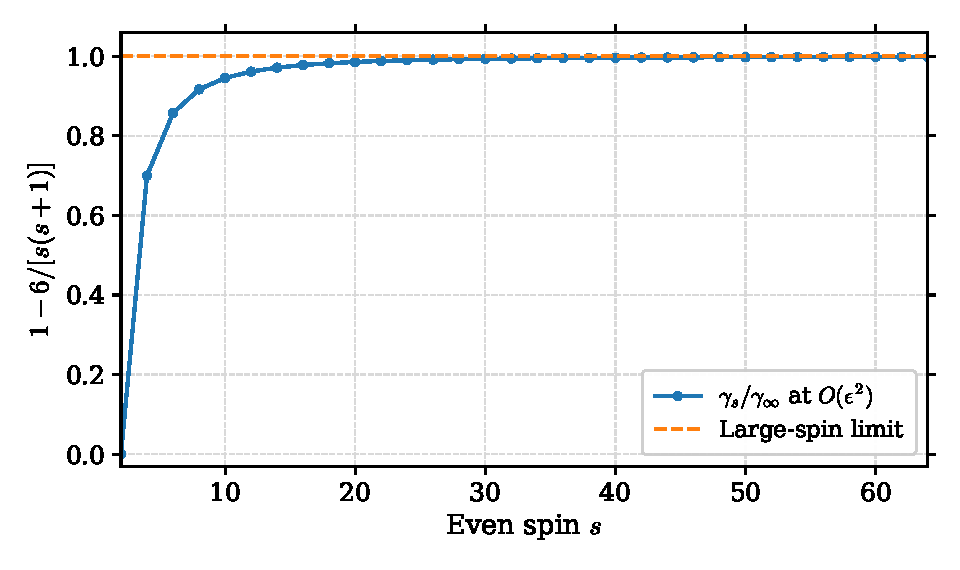
\includegraphics[width=.79\linewidth]{content/FreeElectronQuantumOptics/figures/geometry-highspin/generated/anomalous_spin_profile.pdf}
\caption{$d=4-\epsilon$ 单实标量 Wilson--Fisher 理论领先 $O(\epsilon^2)$ 的偶数自旋比值 $\gamma_S/(\epsilon^2/54)=1-6/[S(S+1)]$。$S=2$ 只作为受保护应力张量的结构检验。}\label{fig:ghs-anomalous-spin-profile}
\end{figure}

\cref{fig:ghs-anomalous-spin-profile} 展示应力张量保护与非保护高自旋维数趋于 $2\gamma_\varphi$ 的衔接；纵轴已经去掉共同的 $\epsilon^2$ 因子，不代表任意维度或任意耦合下的非微扰结果。

可以做三项独立的结构检验。其一，将右侧代数形式延拓至 $S=2$，恰好得到零，与应力张量 Ward 恒等式吻合；但应力张量的实际证明仍来自守恒律，而不是在微扰式上碰巧取零。其二，$S\to\infty$ 时
\begin{equation}\label{eq:ghs-wf-higher-spin-large-s}
 \gamma_S=2\gamma_\varphi-\frac{\epsilon^2}{9S(S+1)}
 +O(\epsilon^3),
\end{equation}
说明大自旋维数逐渐接近两条基本场维数之和加上 $S$，与双扭度的领先结构一致。其三，对首个真正非保护的 $S=4$，
\begin{equation}\label{eq:ghs-wf-spin-four}
 \gamma_4=\frac{7}{540}\epsilon^2+O(\epsilon^3)>0,
\end{equation}
满足幺正性要求。与其把这些检验称作完整证明，更准确的理解是：Ward 恒等式、光锥自举和微扰理论从不同方向同时约束一个已计算出的谱结果。


构造高自旋算符时，常用一个复零极化向量 $z^\mu$ 满足 $z^2=0$，把对称无迹张量缩并为 $J_S(x,z)=J_{\mu_1\cdots\mu_S}(x)z^{\mu_1}\cdots z^{\mu_S}$。由于 $z^2=0$，任意含度规迹的项在 $J_S$ 中消失；但是在求散度时，$\partial/\partial z^\mu$ 会作用于这些项，而它们求导后未必仍然消失。所以先令 $z^2=0$ 再直接使用 $\partial_x\cdot\partial_z$，一般不能代替真实对称无迹张量的散度。

一种与无迹等价类相容的工具是 Thomas 导数
\begin{equation}\label{eq:ghs-thomas-derivative}
 \mathscr D_{z,\mu}
 =\left(\frac d2-1+z\cdot\partial_z\right)\partial_{z^\mu}
 -\frac12 z_\mu\partial_z^2.
\end{equation}
这里 $\mathscr D_z$ 作用在极化向量的齐次多项式上，而不是作用在时空坐标 $x$ 上。计算物理散度时须适当归一化 $\partial_x\cdot\mathscr D_z$ 并处理运动方程与改善项；使用它可以避免把纯迹补偿误判为破坏守恒的算符。自旋二就是重要检验：自由的双线性表达式在加入 $\varphi^4$ 后必须与相互作用的应力张量改善项合并，真正的能动张量才仍然严格守恒。若在这里得到 $\gamma_2\ne0$，应首先核对迹投影与算符混合，而不是怀疑平移 Ward 恒等式。


从一套自由场双线性表达式出发，可以有多个具有相同自旋、对称性和经典维数的复合算符。重整化一般把它们混合：
\begin{equation}\label{eq:ghs-spin-mixing-renormalization}
 [\mathcal O_A]_R=(Z^{-1})_{AB}\mathcal O_{B,0},\qquad
 \Gamma=Z^{-1}\mu_{\mathrm R}\frac{\dd Z}{\dd\mu_{\mathrm R}}\bigg|_{g_0},
\end{equation}
其中 $A,B$ 标记同一扇区的算符，$Z$ 为重整化矩阵，$\Gamma$ 的本征值决定相应的异常维数（其符号须与此处 $Z$ 定义一致）。在存在简并、总导数和运动方程算符时，应先构造规范良好的物理算符商空间，再取有意义的谱。不能仅凭某一个裸插入项的重整化常数，宣称得到一个共形初级的维数。

在固定点上，算符混合的本征值、二点函数的零范数结构和四点函数的共形块分解描述的是同一套谱。\cref{eq:ghs-wf-phi-gamma-result} 给出一个完全由运动方程和 Wick 收缩算出的实例；\cref{eq:ghs-wf-higher-spin-anomalous-result} 给出一条实际可检验的高自旋谱塔；\cref{eq:ghs-wf-higher-spin-large-s} 将它与一般双扭度的大自旋趋势接在一起。高自旋场论研究的价值就在这里：对称性不只是给算符分类，而能把微扰积分、算符代数和非微扰相关函数限制连接为同一个定量问题。

\subsection{低自旋与正交角位置振幅的直接核对}

\begin{example}[最高权球谐的归一化]

在单位球面 $S^{d-1}$ 上写 $z=n^1+\ii n^2$，$|z|^2=(n^1)^2+(n^2)^2$。随机均匀单位向量的前两个分量平方和 $s=|z|^2$ 满足 贝塔分布，其密度正比 $s^{1-1}(1-s)^{(d-2)/2-1}$。于是
\begin{align*}
 \int_{S^{d-1}}\dd\Omega\,|z|^{2k}
 &=\Omega_{d-1}\frac{B(k+1,(d-2)/2)}{B(1,(d-2)/2)}\\
 &=\Omega_{d-1}\frac{\Gamma(k+1)\Gamma(d/2)}{\Gamma(k+d/2)}
 =\Omega_{d-1}\frac{k!}{(d/2)_k}.
\end{align*}
$d=4$ 时这就是 $N_{4,k}=2\pi^2/(k+1)$。角向旋转 $z\mapsto\ee^{\ii\alpha}z$ 意味着对 $k\ne j$，积分 $\int z^k\bar z^j\dd\Omega$ 必须为零。

\end{example}

\begin{example}[四维低自旋的 Fock 范数]

$S=0$ 时，$\mathcal O_0=:\!\varphi^2\!:$，于是 $|\mathcal O_0\rangle=F_0^2(b_0^\dagger)^2|0\rangle$。其中 $F_0^2=1/(4\pi^2)$，所以 $\|\mathcal O_0\|^2=2F_0^4=1/(8\pi^4)=2C_4^2$。

$S=2$ 时，系数 $(c_0,c_1,c_2)=(1,-4,1)$。两种最外侧组合合并后，$|\mathcal O_2\rangle=2F_0F_2 b_0^\dagger b_2^\dagger|0\rangle-4F_1^2(b_1^\dagger)^2|0\rangle$。两者分别贡献 $16/\pi^4$ 与 $32/\pi^4$，因此总范数 $48/\pi^4$，与 \cref{eq:ghs-norm-four-d} 相符。

\end{example}

\begin{example}[正交角位置振幅]

为了计算 \cref{eq:ghs-canonical-vs-field}，不必离散化球面上的微分算符。直接取
\begin{equation*}
 \psi_S(\vb n_1,\vb n_2)
 =\frac{2}{\sqrt{\mathcal N_S}}
 \sum_{k=0}^S B_k\frac{z_1^kz_2^{S-k}}{\sqrt{N_{d,k}N_{d,S-k}}},
 \qquad(S\text{ 偶数}).
\end{equation*}
由于 $\sum_k |B_k|^2=\mathcal N_S/2$，球面正交性给出 $\int|\psi_S|^2=2$。对于 $k=S/2$，这里已经自动包含两个相同玻色模式的 $\sqrt2$ 范数因素；再乘一个对称化因子将重复计数。


\end{example}

标量共形模型把初级条件、粒子态归一化与相关函数数据连成一条可复算的论证。进入电子和规范场的相互作用时，必须重新选用 Dirac 与 Maxwell 自由算子，并加入对应的顶角、外态和测量算符；径向标量态的角权重只有经过这样的耦合模型，才能与具体电子或光子观测联系。
